\documentclass[twoside]{book}

% Packages required by doxygen
\usepackage{calc}
\usepackage{doxygen}
\usepackage{graphicx}
\usepackage[utf8]{inputenc}
\usepackage{makeidx}
\usepackage{multicol}
\usepackage{multirow}
\usepackage{textcomp}
\usepackage[table]{xcolor}

% Font selection
\usepackage[T1]{fontenc}
\usepackage{mathptmx}
\usepackage[scaled=.90]{helvet}
\usepackage{courier}
\usepackage{amssymb}
\usepackage{sectsty}
\renewcommand{\familydefault}{\sfdefault}
\allsectionsfont{%
  \fontseries{bc}\selectfont%
  \color{darkgray}%
}
\renewcommand{\DoxyLabelFont}{%
  \fontseries{bc}\selectfont%
  \color{darkgray}%
}

% Page & text layout
\usepackage{geometry}
\geometry{%
  a4paper,%
  top=2.5cm,%
  bottom=2.5cm,%
  left=2.5cm,%
  right=2.5cm%
}
\tolerance=750
\hfuzz=15pt
\hbadness=750
\setlength{\emergencystretch}{15pt}
\setlength{\parindent}{0cm}
\setlength{\parskip}{0.2cm}
\makeatletter
\renewcommand{\paragraph}{%
  \@startsection{paragraph}{4}{0ex}{-1.0ex}{1.0ex}{%
    \normalfont\normalsize\bfseries\SS@parafont%
  }%
}
\renewcommand{\subparagraph}{%
  \@startsection{subparagraph}{5}{0ex}{-1.0ex}{1.0ex}{%
    \normalfont\normalsize\bfseries\SS@subparafont%
  }%
}
\makeatother

% Headers & footers
\usepackage{fancyhdr}
\pagestyle{fancyplain}
\fancyhead[LE]{\fancyplain{}{\bfseries\thepage}}
\fancyhead[CE]{\fancyplain{}{}}
\fancyhead[RE]{\fancyplain{}{\bfseries\leftmark}}
\fancyhead[LO]{\fancyplain{}{\bfseries\rightmark}}
\fancyhead[CO]{\fancyplain{}{}}
\fancyhead[RO]{\fancyplain{}{\bfseries\thepage}}
\fancyfoot[LE]{\fancyplain{}{}}
\fancyfoot[CE]{\fancyplain{}{}}
\fancyfoot[RE]{\fancyplain{}{\bfseries\scriptsize Generated on Sun Dec 10 2017 19\-:37\-:35 for opt\-\_\-jr\-\_\-doc by Doxygen }}
\fancyfoot[LO]{\fancyplain{}{\bfseries\scriptsize Generated on Sun Dec 10 2017 19\-:37\-:35 for opt\-\_\-jr\-\_\-doc by Doxygen }}
\fancyfoot[CO]{\fancyplain{}{}}
\fancyfoot[RO]{\fancyplain{}{}}
\renewcommand{\footrulewidth}{0.4pt}
\renewcommand{\chaptermark}[1]{%
  \markboth{#1}{}%
}
\renewcommand{\sectionmark}[1]{%
  \markright{\thesection\ #1}%
}

% Indices & bibliography
\usepackage{natbib}
\usepackage[titles]{tocloft}
\setcounter{tocdepth}{3}
\setcounter{secnumdepth}{5}
\makeindex

% Hyperlinks (required, but should be loaded last)
\usepackage{ifpdf}
\ifpdf
  \usepackage[pdftex,pagebackref=true]{hyperref}
\else
  \usepackage[ps2pdf,pagebackref=true]{hyperref}
\fi
\hypersetup{%
  colorlinks=true,%
  linkcolor=blue,%
  citecolor=blue,%
  unicode%
}

% Custom commands
\newcommand{\clearemptydoublepage}{%
  \newpage{\pagestyle{empty}\cleardoublepage}%
}


%===== C O N T E N T S =====

\begin{document}

% Titlepage & ToC
\hypersetup{pageanchor=false}
\pagenumbering{roman}
\begin{titlepage}
\vspace*{7cm}
\begin{center}%
{\Large opt\-\_\-jr\-\_\-doc }\\
\vspace*{1cm}
{\large Generated by Doxygen 1.8.5}\\
\vspace*{0.5cm}
{\small Sun Dec 10 2017 19:37:35}\\
\end{center}
\end{titlepage}
\clearemptydoublepage
\tableofcontents
\clearemptydoublepage
\pagenumbering{arabic}
\hypersetup{pageanchor=true}

%--- Begin generated contents ---
\chapter{P\-A\-C\-S\-\_\-\-P\-R\-O\-J\-E\-C\-T}
\label{md__vagrant_PROJECT_SPARK_PACS_PROJECT_README}
\hypertarget{md__vagrant_PROJECT_SPARK_PACS_PROJECT_README}{}
Program that manage soft deadline application when heavy load occurs. The program reassign the number of core and V\-M to each application. The project is already build in C and the goal is to re-\/write it in C++ with some parallelization (using M\-P\-I and open\-M\-P).

The original project is available at\-: \href{https://github.com/eubr-bigsea/opt_jr}{\tt https\-://github.\-com/eubr-\/bigsea/opt\-\_\-jr}

B\-U\-I\-L\-D D\-O\-C\-U\-M\-E\-N\-T\-A\-T\-I\-O\-N\-:

run in the doc directory\-: doxygen opt\-\_\-jr\-\_\-doxy 
\chapter{Class Index}
\section{Class List}
Here are the classes, structs, unions and interfaces with brief descriptions\-:\begin{DoxyCompactList}
\item\contentsline{section}{\hyperlink{classApplication}{Application} }{\pageref{classApplication}}{}
\item\contentsline{section}{\hyperlink{classBatch}{Batch} }{\pageref{classBatch}}{}
\item\contentsline{section}{\hyperlink{classBounds}{Bounds} }{\pageref{classBounds}}{}
\item\contentsline{section}{\hyperlink{classCandidate}{Candidate} }{\pageref{classCandidate}}{}
\item\contentsline{section}{\hyperlink{classObjFun}{Obj\-Fun} }{\pageref{classObjFun}}{}
\item\contentsline{section}{\hyperlink{classoptJrParameters}{opt\-Jr\-Parameters} }{\pageref{classoptJrParameters}}{}
\item\contentsline{section}{\hyperlink{classsCandidates}{s\-Candidates} }{\pageref{classsCandidates}}{}
\item\contentsline{section}{\hyperlink{classsearch}{search$<$ Policy $>$} }{\pageref{classsearch}}{}
\item\contentsline{section}{\hyperlink{classSearch__alterning}{Search\-\_\-alterning} }{\pageref{classSearch__alterning}}{}
\item\contentsline{section}{\hyperlink{classSearch__methods}{Search\-\_\-methods} }{\pageref{classSearch__methods}}{}
\item\contentsline{section}{\hyperlink{classSearch__selector}{Search\-\_\-selector} }{\pageref{classSearch__selector}}{}
\item\contentsline{section}{\hyperlink{classSearch__separing}{Search\-\_\-separing} }{\pageref{classSearch__separing}}{}
\item\contentsline{section}{\hyperlink{classStatistic}{Statistic} }{\pageref{classStatistic}}{}
\end{DoxyCompactList}

\chapter{File Index}
\section{File List}
Here is a list of all files with brief descriptions\-:\begin{DoxyCompactList}
\item\contentsline{section}{/vagrant/\-P\-R\-O\-J\-E\-C\-T\-\_\-\-S\-P\-A\-R\-K/\-P\-A\-C\-S\-\_\-\-P\-R\-O\-J\-E\-C\-T/opt\-\_\-jr/src/\hyperlink{appByWeight_8cpp}{app\-By\-Weight.\-cpp} }{\pageref{appByWeight_8cpp}}{}
\item\contentsline{section}{/vagrant/\-P\-R\-O\-J\-E\-C\-T\-\_\-\-S\-P\-A\-R\-K/\-P\-A\-C\-S\-\_\-\-P\-R\-O\-J\-E\-C\-T/opt\-\_\-jr/src/\hyperlink{appByWeight_8hh}{app\-By\-Weight.\-hh} }{\pageref{appByWeight_8hh}}{}
\item\contentsline{section}{/vagrant/\-P\-R\-O\-J\-E\-C\-T\-\_\-\-S\-P\-A\-R\-K/\-P\-A\-C\-S\-\_\-\-P\-R\-O\-J\-E\-C\-T/opt\-\_\-jr/src/\hyperlink{application_8cpp}{application.\-cpp} }{\pageref{application_8cpp}}{}
\item\contentsline{section}{/vagrant/\-P\-R\-O\-J\-E\-C\-T\-\_\-\-S\-P\-A\-R\-K/\-P\-A\-C\-S\-\_\-\-P\-R\-O\-J\-E\-C\-T/opt\-\_\-jr/src/\hyperlink{application_8hh}{application.\-hh} }{\pageref{application_8hh}}{}
\item\contentsline{section}{/vagrant/\-P\-R\-O\-J\-E\-C\-T\-\_\-\-S\-P\-A\-R\-K/\-P\-A\-C\-S\-\_\-\-P\-R\-O\-J\-E\-C\-T/opt\-\_\-jr/src/\hyperlink{batch_8cpp}{batch.\-cpp} }{\pageref{batch_8cpp}}{}
\item\contentsline{section}{/vagrant/\-P\-R\-O\-J\-E\-C\-T\-\_\-\-S\-P\-A\-R\-K/\-P\-A\-C\-S\-\_\-\-P\-R\-O\-J\-E\-C\-T/opt\-\_\-jr/src/\hyperlink{batch_8hh}{batch.\-hh} }{\pageref{batch_8hh}}{}
\item\contentsline{section}{/vagrant/\-P\-R\-O\-J\-E\-C\-T\-\_\-\-S\-P\-A\-R\-K/\-P\-A\-C\-S\-\_\-\-P\-R\-O\-J\-E\-C\-T/opt\-\_\-jr/src/\hyperlink{bounds_8cpp}{bounds.\-cpp} }{\pageref{bounds_8cpp}}{}
\item\contentsline{section}{/vagrant/\-P\-R\-O\-J\-E\-C\-T\-\_\-\-S\-P\-A\-R\-K/\-P\-A\-C\-S\-\_\-\-P\-R\-O\-J\-E\-C\-T/opt\-\_\-jr/src/\hyperlink{bounds_8hh}{bounds.\-hh} }{\pageref{bounds_8hh}}{}
\item\contentsline{section}{/vagrant/\-P\-R\-O\-J\-E\-C\-T\-\_\-\-S\-P\-A\-R\-K/\-P\-A\-C\-S\-\_\-\-P\-R\-O\-J\-E\-C\-T/opt\-\_\-jr/src/\hyperlink{candidates_8cpp}{candidates.\-cpp} }{\pageref{candidates_8cpp}}{}
\item\contentsline{section}{/vagrant/\-P\-R\-O\-J\-E\-C\-T\-\_\-\-S\-P\-A\-R\-K/\-P\-A\-C\-S\-\_\-\-P\-R\-O\-J\-E\-C\-T/opt\-\_\-jr/src/\hyperlink{candidates_8hh}{candidates.\-hh} }{\pageref{candidates_8hh}}{}
\item\contentsline{section}{/vagrant/\-P\-R\-O\-J\-E\-C\-T\-\_\-\-S\-P\-A\-R\-K/\-P\-A\-C\-S\-\_\-\-P\-R\-O\-J\-E\-C\-T/opt\-\_\-jr/src/\hyperlink{db_8cpp}{db.\-cpp} }{\pageref{db_8cpp}}{}
\item\contentsline{section}{/vagrant/\-P\-R\-O\-J\-E\-C\-T\-\_\-\-S\-P\-A\-R\-K/\-P\-A\-C\-S\-\_\-\-P\-R\-O\-J\-E\-C\-T/opt\-\_\-jr/src/\hyperlink{db_8hh}{db.\-hh} }{\pageref{db_8hh}}{}
\item\contentsline{section}{/vagrant/\-P\-R\-O\-J\-E\-C\-T\-\_\-\-S\-P\-A\-R\-K/\-P\-A\-C\-S\-\_\-\-P\-R\-O\-J\-E\-C\-T/opt\-\_\-jr/src/\hyperlink{debugmessage_8cpp}{debugmessage.\-cpp} }{\pageref{debugmessage_8cpp}}{}
\item\contentsline{section}{/vagrant/\-P\-R\-O\-J\-E\-C\-T\-\_\-\-S\-P\-A\-R\-K/\-P\-A\-C\-S\-\_\-\-P\-R\-O\-J\-E\-C\-T/opt\-\_\-jr/src/\hyperlink{debugmessage_8hh}{debugmessage.\-hh} }{\pageref{debugmessage_8hh}}{}
\item\contentsline{section}{/vagrant/\-P\-R\-O\-J\-E\-C\-T\-\_\-\-S\-P\-A\-R\-K/\-P\-A\-C\-S\-\_\-\-P\-R\-O\-J\-E\-C\-T/opt\-\_\-jr/src/\hyperlink{invokePredictor_8cpp}{invoke\-Predictor.\-cpp} }{\pageref{invokePredictor_8cpp}}{}
\item\contentsline{section}{/vagrant/\-P\-R\-O\-J\-E\-C\-T\-\_\-\-S\-P\-A\-R\-K/\-P\-A\-C\-S\-\_\-\-P\-R\-O\-J\-E\-C\-T/opt\-\_\-jr/src/\hyperlink{invokePredictor_8hh}{invoke\-Predictor.\-hh} }{\pageref{invokePredictor_8hh}}{}
\item\contentsline{section}{/vagrant/\-P\-R\-O\-J\-E\-C\-T\-\_\-\-S\-P\-A\-R\-K/\-P\-A\-C\-S\-\_\-\-P\-R\-O\-J\-E\-C\-T/opt\-\_\-jr/src/\hyperlink{invokePredictor__helper_8cpp}{invoke\-Predictor\-\_\-helper.\-cpp} }{\pageref{invokePredictor__helper_8cpp}}{}
\item\contentsline{section}{/vagrant/\-P\-R\-O\-J\-E\-C\-T\-\_\-\-S\-P\-A\-R\-K/\-P\-A\-C\-S\-\_\-\-P\-R\-O\-J\-E\-C\-T/opt\-\_\-jr/src/\hyperlink{invokePredictor__helper_8hh}{invoke\-Predictor\-\_\-helper.\-hh} }{\pageref{invokePredictor__helper_8hh}}{}
\item\contentsline{section}{/vagrant/\-P\-R\-O\-J\-E\-C\-T\-\_\-\-S\-P\-A\-R\-K/\-P\-A\-C\-S\-\_\-\-P\-R\-O\-J\-E\-C\-T/opt\-\_\-jr/src/\hyperlink{main_8cpp}{main.\-cpp} }{\pageref{main_8cpp}}{}
\item\contentsline{section}{/vagrant/\-P\-R\-O\-J\-E\-C\-T\-\_\-\-S\-P\-A\-R\-K/\-P\-A\-C\-S\-\_\-\-P\-R\-O\-J\-E\-C\-T/opt\-\_\-jr/src/\hyperlink{objectiveFunction_8cpp}{objective\-Function.\-cpp} }{\pageref{objectiveFunction_8cpp}}{}
\item\contentsline{section}{/vagrant/\-P\-R\-O\-J\-E\-C\-T\-\_\-\-S\-P\-A\-R\-K/\-P\-A\-C\-S\-\_\-\-P\-R\-O\-J\-E\-C\-T/opt\-\_\-jr/src/\hyperlink{objectiveFunction_8hh}{objective\-Function.\-hh} }{\pageref{objectiveFunction_8hh}}{}
\item\contentsline{section}{/vagrant/\-P\-R\-O\-J\-E\-C\-T\-\_\-\-S\-P\-A\-R\-K/\-P\-A\-C\-S\-\_\-\-P\-R\-O\-J\-E\-C\-T/opt\-\_\-jr/src/\hyperlink{optjrParam__helper_8cpp}{optjr\-Param\-\_\-helper.\-cpp} }{\pageref{optjrParam__helper_8cpp}}{}
\item\contentsline{section}{/vagrant/\-P\-R\-O\-J\-E\-C\-T\-\_\-\-S\-P\-A\-R\-K/\-P\-A\-C\-S\-\_\-\-P\-R\-O\-J\-E\-C\-T/opt\-\_\-jr/src/\hyperlink{optjrParam__helper_8hh}{optjr\-Param\-\_\-helper.\-hh} }{\pageref{optjrParam__helper_8hh}}{}
\item\contentsline{section}{/vagrant/\-P\-R\-O\-J\-E\-C\-T\-\_\-\-S\-P\-A\-R\-K/\-P\-A\-C\-S\-\_\-\-P\-R\-O\-J\-E\-C\-T/opt\-\_\-jr/src/\hyperlink{optjrparameters_8cpp}{optjrparameters.\-cpp} }{\pageref{optjrparameters_8cpp}}{}
\item\contentsline{section}{/vagrant/\-P\-R\-O\-J\-E\-C\-T\-\_\-\-S\-P\-A\-R\-K/\-P\-A\-C\-S\-\_\-\-P\-R\-O\-J\-E\-C\-T/opt\-\_\-jr/src/\hyperlink{optjrParameters_8hh}{optjr\-Parameters.\-hh} }{\pageref{optjrParameters_8hh}}{}
\item\contentsline{section}{/vagrant/\-P\-R\-O\-J\-E\-C\-T\-\_\-\-S\-P\-A\-R\-K/\-P\-A\-C\-S\-\_\-\-P\-R\-O\-J\-E\-C\-T/opt\-\_\-jr/src/\hyperlink{read__app__file_8cpp}{read\-\_\-app\-\_\-file.\-cpp} }{\pageref{read__app__file_8cpp}}{}
\item\contentsline{section}{/vagrant/\-P\-R\-O\-J\-E\-C\-T\-\_\-\-S\-P\-A\-R\-K/\-P\-A\-C\-S\-\_\-\-P\-R\-O\-J\-E\-C\-T/opt\-\_\-jr/src/\hyperlink{read__app__file_8hh}{read\-\_\-app\-\_\-file.\-hh} }{\pageref{read__app__file_8hh}}{}
\item\contentsline{section}{/vagrant/\-P\-R\-O\-J\-E\-C\-T\-\_\-\-S\-P\-A\-R\-K/\-P\-A\-C\-S\-\_\-\-P\-R\-O\-J\-E\-C\-T/opt\-\_\-jr/src/\hyperlink{readConfigurationFile_8cpp}{read\-Configuration\-File.\-cpp} }{\pageref{readConfigurationFile_8cpp}}{}
\item\contentsline{section}{/vagrant/\-P\-R\-O\-J\-E\-C\-T\-\_\-\-S\-P\-A\-R\-K/\-P\-A\-C\-S\-\_\-\-P\-R\-O\-J\-E\-C\-T/opt\-\_\-jr/src/\hyperlink{readConfigurationFile_8hh}{read\-Configuration\-File.\-hh} }{\pageref{readConfigurationFile_8hh}}{}
\item\contentsline{section}{/vagrant/\-P\-R\-O\-J\-E\-C\-T\-\_\-\-S\-P\-A\-R\-K/\-P\-A\-C\-S\-\_\-\-P\-R\-O\-J\-E\-C\-T/opt\-\_\-jr/src/\hyperlink{search_8cpp}{search.\-cpp} }{\pageref{search_8cpp}}{}
\item\contentsline{section}{/vagrant/\-P\-R\-O\-J\-E\-C\-T\-\_\-\-S\-P\-A\-R\-K/\-P\-A\-C\-S\-\_\-\-P\-R\-O\-J\-E\-C\-T/opt\-\_\-jr/src/\hyperlink{search_8hh}{search.\-hh} }{\pageref{search_8hh}}{}
\item\contentsline{section}{/vagrant/\-P\-R\-O\-J\-E\-C\-T\-\_\-\-S\-P\-A\-R\-K/\-P\-A\-C\-S\-\_\-\-P\-R\-O\-J\-E\-C\-T/opt\-\_\-jr/src/\hyperlink{utility_8cpp}{utility.\-cpp} }{\pageref{utility_8cpp}}{}
\item\contentsline{section}{/vagrant/\-P\-R\-O\-J\-E\-C\-T\-\_\-\-S\-P\-A\-R\-K/\-P\-A\-C\-S\-\_\-\-P\-R\-O\-J\-E\-C\-T/opt\-\_\-jr/src/\hyperlink{utility_8hh}{utility.\-hh} }{\pageref{utility_8hh}}{}
\end{DoxyCompactList}

\chapter{Class Documentation}
\hypertarget{classApplication}{\section{Application Class Reference}
\label{classApplication}\index{Application@{Application}}
}


{\ttfamily \#include $<$application.\-hh$>$}



Collaboration diagram for Application\-:\nopagebreak
\begin{figure}[H]
\begin{center}
\leavevmode
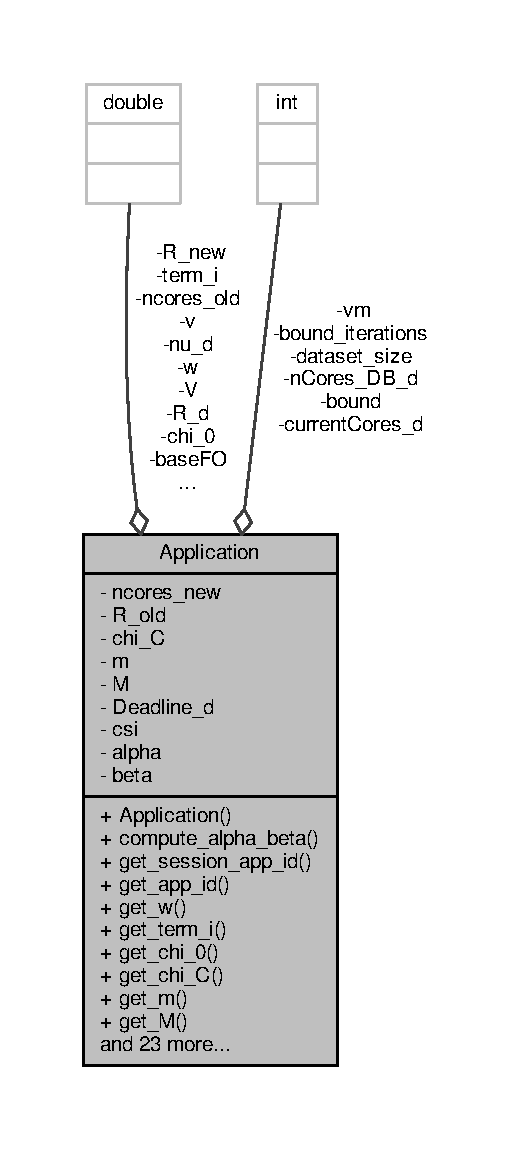
\includegraphics[width=309pt]{classApplication__coll__graph}
\end{center}
\end{figure}
\subsection*{Public Member Functions}
\begin{DoxyCompactItemize}
\item 
\hyperlink{classApplication_aa660e2135b162cfddaca0918be8599e8}{Application} (std\-::string \hyperlink{classApplication_a5e28ffadb86925ecae57ab18c0085d90}{session\-\_\-app\-\_\-id}, std\-::string \hyperlink{classApplication_a05377e6cdcb9d48f29e0f1972a4a16fe}{app\-\_\-id}, double \hyperlink{classApplication_aead1b7b0150c2a3ebd6c36b1db8c4732}{w}, double \hyperlink{classApplication_a3b9dab40d189989c836b8d328946bbb6}{chi\-\_\-0}, double \hyperlink{classApplication_a46e29a6bfc74de610feec809a77dfb62}{chi\-\_\-\-C}, double \hyperlink{classApplication_ab903d83d3cde51569a27f97752c9f158}{m}, double \hyperlink{classApplication_a14904a2abf46cc0a50eb82043fa0912e}{M}, double \hyperlink{classApplication_aa92ad37e6701931176e0dc9b260fd7ee}{V}, double \hyperlink{classApplication_a9efc167094a42382504dd28a7ac402e0}{v}, double D, double \hyperlink{classApplication_a20adc533c6b6147342b3f60dc0fbd9bc}{csi}, std\-::string St, int Dataset\-Size)
\item 
double \hyperlink{classApplication_a97054cee52b315da040098c3927c909e}{Obj\-Function\-Component} (\hyperlink{readConfigurationFile_8hh_ab8f35b1da3261263c5e9c0e7c8921f5c}{s\-Configuration} \&configuration, M\-Y\-S\-Q\-L $\ast$conn, \hyperlink{classoptJrParameters}{opt\-Jr\-Parameters} \&par)
\end{DoxyCompactItemize}
\subsection*{Public Attributes}
\begin{DoxyCompactItemize}
\item 
int \hyperlink{classApplication_abc7e87e8cbe2e64fa4e2ff2afdf7a4fc}{mode}
\item 
std\-::string \hyperlink{classApplication_a5e28ffadb86925ecae57ab18c0085d90}{session\-\_\-app\-\_\-id}
\item 
std\-::string \hyperlink{classApplication_a05377e6cdcb9d48f29e0f1972a4a16fe}{app\-\_\-id}
\item 
double \hyperlink{classApplication_aead1b7b0150c2a3ebd6c36b1db8c4732}{w}
\item 
double \hyperlink{classApplication_ad5486702327ad61e56ed04fb54d58c20}{term\-\_\-i}
\item 
double \hyperlink{classApplication_a3b9dab40d189989c836b8d328946bbb6}{chi\-\_\-0}
\item 
double \hyperlink{classApplication_a46e29a6bfc74de610feec809a77dfb62}{chi\-\_\-\-C}
\item 
double \hyperlink{classApplication_ab903d83d3cde51569a27f97752c9f158}{m}
\item 
double \hyperlink{classApplication_a14904a2abf46cc0a50eb82043fa0912e}{M}
\item 
double \hyperlink{classApplication_aa92ad37e6701931176e0dc9b260fd7ee}{V}
\item 
double \hyperlink{classApplication_a9efc167094a42382504dd28a7ac402e0}{v}
\item 
double \hyperlink{classApplication_a2a989ae288a74ee5250b5acf449c864a}{Deadline\-\_\-d}
\item 
double \hyperlink{classApplication_a20adc533c6b6147342b3f60dc0fbd9bc}{csi}
\item 
std\-::string \hyperlink{classApplication_adb1cba2c06695bfdf81482dfba449d5b}{stage}
\item 
int \hyperlink{classApplication_aaa155e818d807f585d83ecacf4abfe42}{dataset\-Size}
\item 
double \hyperlink{classApplication_a42c22b9a3130cf1f2722ce222f2e5bae}{nu\-\_\-d}
\item 
int \hyperlink{classApplication_adee341a84a5389dfd4d16e7f8e697190}{current\-Cores\-\_\-d}
\item 
int \hyperlink{classApplication_a95104d330c9c7ed2c1017b4938a39a9a}{n\-Cores\-\_\-\-D\-B\-\_\-d}
\item 
int \hyperlink{classApplication_a6e91bef9d503af0e8ba38c8f445c8cb0}{bound}
\item 
double \hyperlink{classApplication_a374d43f68ae27aaed98278e8152a434c}{R\-\_\-d}
\item 
double \hyperlink{classApplication_a32da2e06513ef910601d75eb89bb528b}{R\-\_\-bound\-\_\-d}
\item 
double \hyperlink{classApplication_aa703e7525d446d98b5cd51c959d35998}{base\-F\-O}
\item 
double \hyperlink{classApplication_a95fd54cbed658fb23ce27939666c91d2}{initial\-Base\-F\-O}
\item 
float \hyperlink{classApplication_a087ef34a09792f2954940324dcea20d6}{alpha}
\item 
float \hyperlink{classApplication_a7c74ef816a425a4115005d15d01ac9c6}{beta}
\item 
\hyperlink{classsAlphaBetaManagement}{s\-Alpha\-Beta\-Management} \hyperlink{classApplication_a6bbd698f2df7c4cedb9fb46fce23dbfe}{s\-A\-B}
\item 
int \hyperlink{classApplication_a6a3692743eccba602a58fdfc3f23950b}{bound\-Iterations}
\item 
int \hyperlink{classApplication_a0a3fe386eb8244e536bc5297709d1269}{vm}
\end{DoxyCompactItemize}


\subsection{Constructor \& Destructor Documentation}
\hypertarget{classApplication_aa660e2135b162cfddaca0918be8599e8}{\index{Application@{Application}!Application@{Application}}
\index{Application@{Application}!Application@{Application}}
\subsubsection[{Application}]{\setlength{\rightskip}{0pt plus 5cm}Application\-::\-Application (
\begin{DoxyParamCaption}
\item[{std\-::string}]{session\-\_\-app\-\_\-id, }
\item[{std\-::string}]{app\-\_\-id, }
\item[{double}]{w, }
\item[{double}]{chi\-\_\-0, }
\item[{double}]{chi\-\_\-\-C, }
\item[{double}]{m, }
\item[{double}]{M, }
\item[{double}]{V, }
\item[{double}]{v, }
\item[{double}]{D, }
\item[{double}]{csi, }
\item[{std\-::string}]{St, }
\item[{int}]{Dataset\-Size}
\end{DoxyParamCaption}
)}}\label{classApplication_aa660e2135b162cfddaca0918be8599e8}


\subsection{Member Function Documentation}
\hypertarget{classApplication_a97054cee52b315da040098c3927c909e}{\index{Application@{Application}!Obj\-Function\-Component@{Obj\-Function\-Component}}
\index{Obj\-Function\-Component@{Obj\-Function\-Component}!Application@{Application}}
\subsubsection[{Obj\-Function\-Component}]{\setlength{\rightskip}{0pt plus 5cm}double Application\-::\-Obj\-Function\-Component (
\begin{DoxyParamCaption}
\item[{{\bf s\-Configuration} \&}]{configuration, }
\item[{M\-Y\-S\-Q\-L $\ast$}]{conn, }
\item[{{\bf opt\-Jr\-Parameters} \&}]{par}
\end{DoxyParamCaption}
)}}\label{classApplication_a97054cee52b315da040098c3927c909e}


Here is the call graph for this function\-:\nopagebreak
\begin{figure}[H]
\begin{center}
\leavevmode
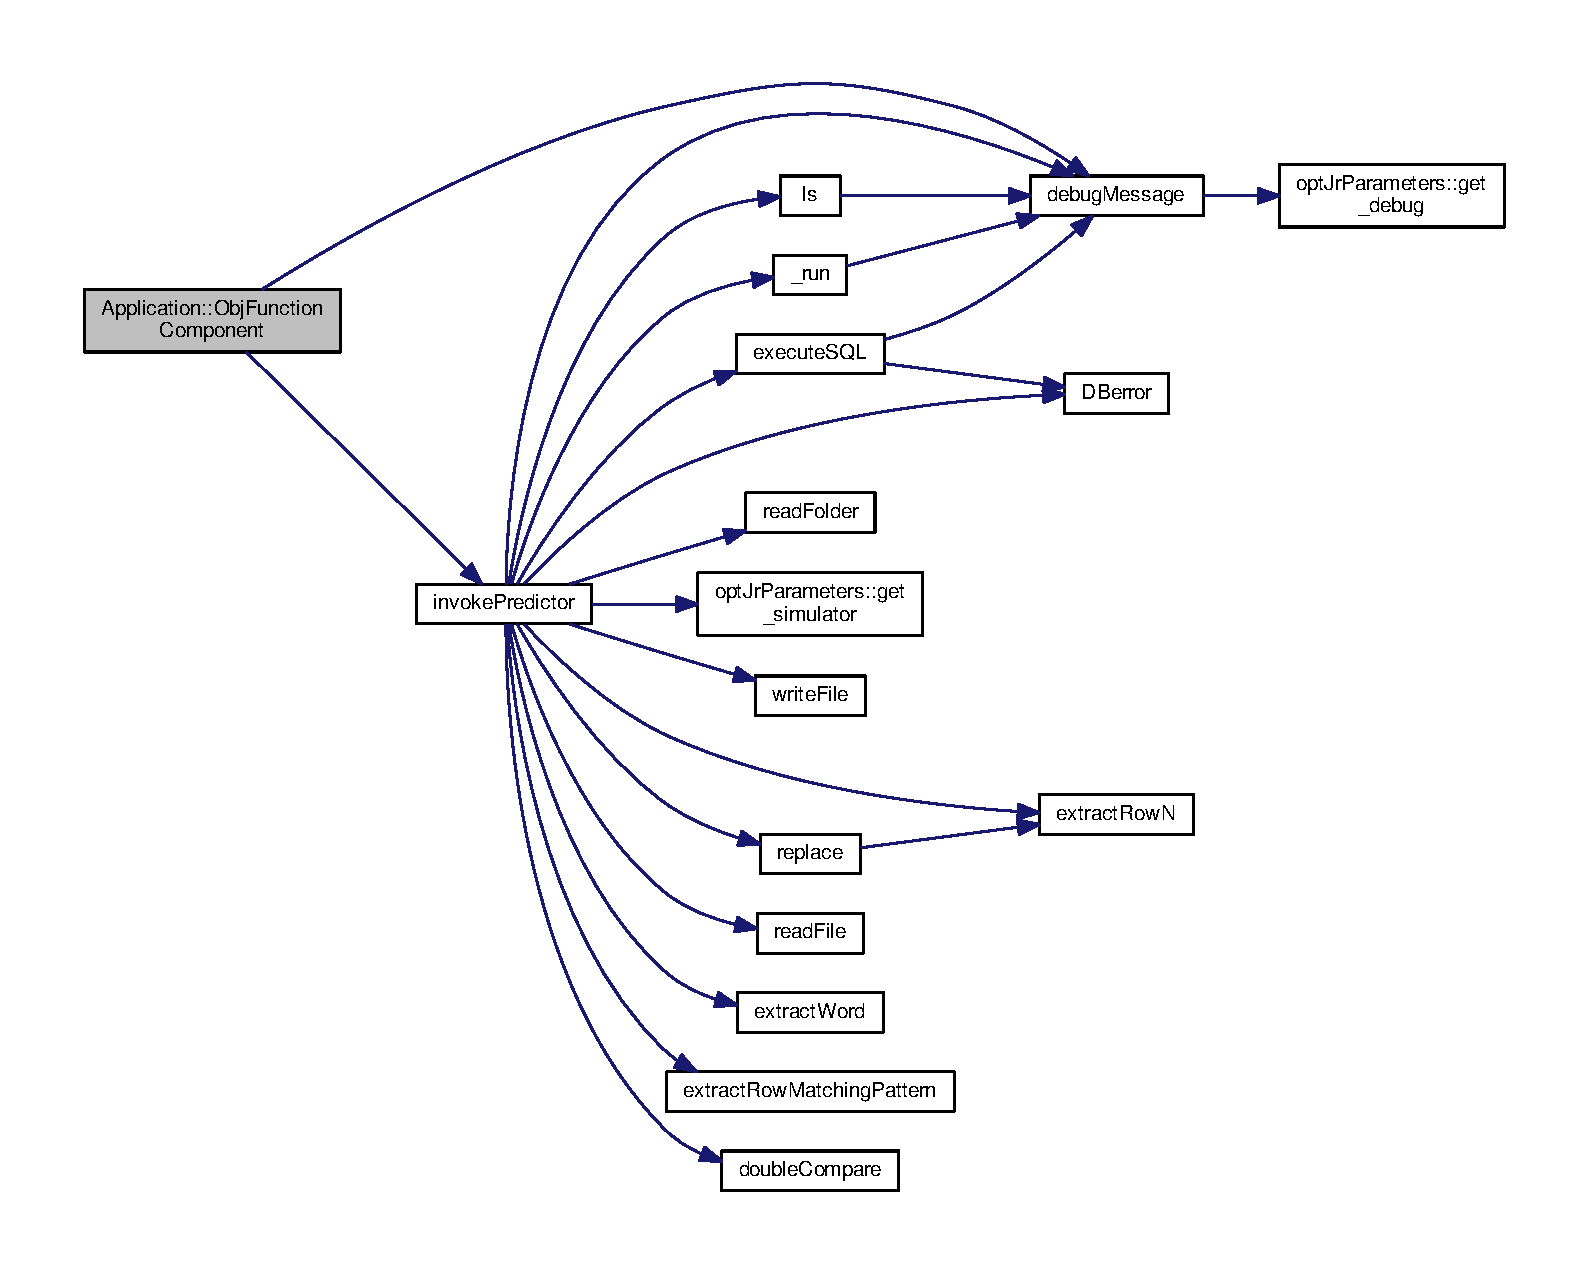
\includegraphics[width=350pt]{classApplication_a97054cee52b315da040098c3927c909e_cgraph}
\end{center}
\end{figure}




\subsection{Member Data Documentation}
\hypertarget{classApplication_a087ef34a09792f2954940324dcea20d6}{\index{Application@{Application}!alpha@{alpha}}
\index{alpha@{alpha}!Application@{Application}}
\subsubsection[{alpha}]{\setlength{\rightskip}{0pt plus 5cm}float Application\-::alpha}}\label{classApplication_a087ef34a09792f2954940324dcea20d6}
\hypertarget{classApplication_a05377e6cdcb9d48f29e0f1972a4a16fe}{\index{Application@{Application}!app\-\_\-id@{app\-\_\-id}}
\index{app\-\_\-id@{app\-\_\-id}!Application@{Application}}
\subsubsection[{app\-\_\-id}]{\setlength{\rightskip}{0pt plus 5cm}std\-::string Application\-::app\-\_\-id}}\label{classApplication_a05377e6cdcb9d48f29e0f1972a4a16fe}
\hypertarget{classApplication_aa703e7525d446d98b5cd51c959d35998}{\index{Application@{Application}!base\-F\-O@{base\-F\-O}}
\index{base\-F\-O@{base\-F\-O}!Application@{Application}}
\subsubsection[{base\-F\-O}]{\setlength{\rightskip}{0pt plus 5cm}double Application\-::base\-F\-O}}\label{classApplication_aa703e7525d446d98b5cd51c959d35998}
\hypertarget{classApplication_a7c74ef816a425a4115005d15d01ac9c6}{\index{Application@{Application}!beta@{beta}}
\index{beta@{beta}!Application@{Application}}
\subsubsection[{beta}]{\setlength{\rightskip}{0pt plus 5cm}float Application\-::beta}}\label{classApplication_a7c74ef816a425a4115005d15d01ac9c6}
\hypertarget{classApplication_a6e91bef9d503af0e8ba38c8f445c8cb0}{\index{Application@{Application}!bound@{bound}}
\index{bound@{bound}!Application@{Application}}
\subsubsection[{bound}]{\setlength{\rightskip}{0pt plus 5cm}int Application\-::bound}}\label{classApplication_a6e91bef9d503af0e8ba38c8f445c8cb0}
\hypertarget{classApplication_a6a3692743eccba602a58fdfc3f23950b}{\index{Application@{Application}!bound\-Iterations@{bound\-Iterations}}
\index{bound\-Iterations@{bound\-Iterations}!Application@{Application}}
\subsubsection[{bound\-Iterations}]{\setlength{\rightskip}{0pt plus 5cm}int Application\-::bound\-Iterations}}\label{classApplication_a6a3692743eccba602a58fdfc3f23950b}
\hypertarget{classApplication_a3b9dab40d189989c836b8d328946bbb6}{\index{Application@{Application}!chi\-\_\-0@{chi\-\_\-0}}
\index{chi\-\_\-0@{chi\-\_\-0}!Application@{Application}}
\subsubsection[{chi\-\_\-0}]{\setlength{\rightskip}{0pt plus 5cm}double Application\-::chi\-\_\-0}}\label{classApplication_a3b9dab40d189989c836b8d328946bbb6}
\hypertarget{classApplication_a46e29a6bfc74de610feec809a77dfb62}{\index{Application@{Application}!chi\-\_\-\-C@{chi\-\_\-\-C}}
\index{chi\-\_\-\-C@{chi\-\_\-\-C}!Application@{Application}}
\subsubsection[{chi\-\_\-\-C}]{\setlength{\rightskip}{0pt plus 5cm}double Application\-::chi\-\_\-\-C}}\label{classApplication_a46e29a6bfc74de610feec809a77dfb62}
\hypertarget{classApplication_a20adc533c6b6147342b3f60dc0fbd9bc}{\index{Application@{Application}!csi@{csi}}
\index{csi@{csi}!Application@{Application}}
\subsubsection[{csi}]{\setlength{\rightskip}{0pt plus 5cm}double Application\-::csi}}\label{classApplication_a20adc533c6b6147342b3f60dc0fbd9bc}
\hypertarget{classApplication_adee341a84a5389dfd4d16e7f8e697190}{\index{Application@{Application}!current\-Cores\-\_\-d@{current\-Cores\-\_\-d}}
\index{current\-Cores\-\_\-d@{current\-Cores\-\_\-d}!Application@{Application}}
\subsubsection[{current\-Cores\-\_\-d}]{\setlength{\rightskip}{0pt plus 5cm}int Application\-::current\-Cores\-\_\-d}}\label{classApplication_adee341a84a5389dfd4d16e7f8e697190}
\hypertarget{classApplication_aaa155e818d807f585d83ecacf4abfe42}{\index{Application@{Application}!dataset\-Size@{dataset\-Size}}
\index{dataset\-Size@{dataset\-Size}!Application@{Application}}
\subsubsection[{dataset\-Size}]{\setlength{\rightskip}{0pt plus 5cm}int Application\-::dataset\-Size}}\label{classApplication_aaa155e818d807f585d83ecacf4abfe42}
\hypertarget{classApplication_a2a989ae288a74ee5250b5acf449c864a}{\index{Application@{Application}!Deadline\-\_\-d@{Deadline\-\_\-d}}
\index{Deadline\-\_\-d@{Deadline\-\_\-d}!Application@{Application}}
\subsubsection[{Deadline\-\_\-d}]{\setlength{\rightskip}{0pt plus 5cm}double Application\-::\-Deadline\-\_\-d}}\label{classApplication_a2a989ae288a74ee5250b5acf449c864a}
\hypertarget{classApplication_a95fd54cbed658fb23ce27939666c91d2}{\index{Application@{Application}!initial\-Base\-F\-O@{initial\-Base\-F\-O}}
\index{initial\-Base\-F\-O@{initial\-Base\-F\-O}!Application@{Application}}
\subsubsection[{initial\-Base\-F\-O}]{\setlength{\rightskip}{0pt plus 5cm}double Application\-::initial\-Base\-F\-O}}\label{classApplication_a95fd54cbed658fb23ce27939666c91d2}
\hypertarget{classApplication_ab903d83d3cde51569a27f97752c9f158}{\index{Application@{Application}!m@{m}}
\index{m@{m}!Application@{Application}}
\subsubsection[{m}]{\setlength{\rightskip}{0pt plus 5cm}double Application\-::m}}\label{classApplication_ab903d83d3cde51569a27f97752c9f158}
\hypertarget{classApplication_a14904a2abf46cc0a50eb82043fa0912e}{\index{Application@{Application}!M@{M}}
\index{M@{M}!Application@{Application}}
\subsubsection[{M}]{\setlength{\rightskip}{0pt plus 5cm}double Application\-::\-M}}\label{classApplication_a14904a2abf46cc0a50eb82043fa0912e}
\hypertarget{classApplication_abc7e87e8cbe2e64fa4e2ff2afdf7a4fc}{\index{Application@{Application}!mode@{mode}}
\index{mode@{mode}!Application@{Application}}
\subsubsection[{mode}]{\setlength{\rightskip}{0pt plus 5cm}int Application\-::mode}}\label{classApplication_abc7e87e8cbe2e64fa4e2ff2afdf7a4fc}
\hypertarget{classApplication_a95104d330c9c7ed2c1017b4938a39a9a}{\index{Application@{Application}!n\-Cores\-\_\-\-D\-B\-\_\-d@{n\-Cores\-\_\-\-D\-B\-\_\-d}}
\index{n\-Cores\-\_\-\-D\-B\-\_\-d@{n\-Cores\-\_\-\-D\-B\-\_\-d}!Application@{Application}}
\subsubsection[{n\-Cores\-\_\-\-D\-B\-\_\-d}]{\setlength{\rightskip}{0pt plus 5cm}int Application\-::n\-Cores\-\_\-\-D\-B\-\_\-d}}\label{classApplication_a95104d330c9c7ed2c1017b4938a39a9a}
\hypertarget{classApplication_a42c22b9a3130cf1f2722ce222f2e5bae}{\index{Application@{Application}!nu\-\_\-d@{nu\-\_\-d}}
\index{nu\-\_\-d@{nu\-\_\-d}!Application@{Application}}
\subsubsection[{nu\-\_\-d}]{\setlength{\rightskip}{0pt plus 5cm}double Application\-::nu\-\_\-d}}\label{classApplication_a42c22b9a3130cf1f2722ce222f2e5bae}
\hypertarget{classApplication_a32da2e06513ef910601d75eb89bb528b}{\index{Application@{Application}!R\-\_\-bound\-\_\-d@{R\-\_\-bound\-\_\-d}}
\index{R\-\_\-bound\-\_\-d@{R\-\_\-bound\-\_\-d}!Application@{Application}}
\subsubsection[{R\-\_\-bound\-\_\-d}]{\setlength{\rightskip}{0pt plus 5cm}double Application\-::\-R\-\_\-bound\-\_\-d}}\label{classApplication_a32da2e06513ef910601d75eb89bb528b}
\hypertarget{classApplication_a374d43f68ae27aaed98278e8152a434c}{\index{Application@{Application}!R\-\_\-d@{R\-\_\-d}}
\index{R\-\_\-d@{R\-\_\-d}!Application@{Application}}
\subsubsection[{R\-\_\-d}]{\setlength{\rightskip}{0pt plus 5cm}double Application\-::\-R\-\_\-d}}\label{classApplication_a374d43f68ae27aaed98278e8152a434c}
\hypertarget{classApplication_a6bbd698f2df7c4cedb9fb46fce23dbfe}{\index{Application@{Application}!s\-A\-B@{s\-A\-B}}
\index{s\-A\-B@{s\-A\-B}!Application@{Application}}
\subsubsection[{s\-A\-B}]{\setlength{\rightskip}{0pt plus 5cm}{\bf s\-Alpha\-Beta\-Management} Application\-::s\-A\-B}}\label{classApplication_a6bbd698f2df7c4cedb9fb46fce23dbfe}
\hypertarget{classApplication_a5e28ffadb86925ecae57ab18c0085d90}{\index{Application@{Application}!session\-\_\-app\-\_\-id@{session\-\_\-app\-\_\-id}}
\index{session\-\_\-app\-\_\-id@{session\-\_\-app\-\_\-id}!Application@{Application}}
\subsubsection[{session\-\_\-app\-\_\-id}]{\setlength{\rightskip}{0pt plus 5cm}std\-::string Application\-::session\-\_\-app\-\_\-id}}\label{classApplication_a5e28ffadb86925ecae57ab18c0085d90}
\hypertarget{classApplication_adb1cba2c06695bfdf81482dfba449d5b}{\index{Application@{Application}!stage@{stage}}
\index{stage@{stage}!Application@{Application}}
\subsubsection[{stage}]{\setlength{\rightskip}{0pt plus 5cm}std\-::string Application\-::stage}}\label{classApplication_adb1cba2c06695bfdf81482dfba449d5b}
\hypertarget{classApplication_ad5486702327ad61e56ed04fb54d58c20}{\index{Application@{Application}!term\-\_\-i@{term\-\_\-i}}
\index{term\-\_\-i@{term\-\_\-i}!Application@{Application}}
\subsubsection[{term\-\_\-i}]{\setlength{\rightskip}{0pt plus 5cm}double Application\-::term\-\_\-i}}\label{classApplication_ad5486702327ad61e56ed04fb54d58c20}
\hypertarget{classApplication_aa92ad37e6701931176e0dc9b260fd7ee}{\index{Application@{Application}!V@{V}}
\index{V@{V}!Application@{Application}}
\subsubsection[{V}]{\setlength{\rightskip}{0pt plus 5cm}double Application\-::\-V}}\label{classApplication_aa92ad37e6701931176e0dc9b260fd7ee}
\hypertarget{classApplication_a9efc167094a42382504dd28a7ac402e0}{\index{Application@{Application}!v@{v}}
\index{v@{v}!Application@{Application}}
\subsubsection[{v}]{\setlength{\rightskip}{0pt plus 5cm}double Application\-::v}}\label{classApplication_a9efc167094a42382504dd28a7ac402e0}
\hypertarget{classApplication_a0a3fe386eb8244e536bc5297709d1269}{\index{Application@{Application}!vm@{vm}}
\index{vm@{vm}!Application@{Application}}
\subsubsection[{vm}]{\setlength{\rightskip}{0pt plus 5cm}int Application\-::vm}}\label{classApplication_a0a3fe386eb8244e536bc5297709d1269}
\hypertarget{classApplication_aead1b7b0150c2a3ebd6c36b1db8c4732}{\index{Application@{Application}!w@{w}}
\index{w@{w}!Application@{Application}}
\subsubsection[{w}]{\setlength{\rightskip}{0pt plus 5cm}double Application\-::w}}\label{classApplication_aead1b7b0150c2a3ebd6c36b1db8c4732}


The documentation for this class was generated from the following files\-:\begin{DoxyCompactItemize}
\item 
/vagrant/\-P\-R\-O\-J\-E\-C\-T\-\_\-\-S\-P\-A\-R\-K/\-P\-A\-C\-S\-\_\-\-P\-R\-O\-J\-E\-C\-T/opt\-\_\-jr/src/\hyperlink{application_8hh}{application.\-hh}\item 
/vagrant/\-P\-R\-O\-J\-E\-C\-T\-\_\-\-S\-P\-A\-R\-K/\-P\-A\-C\-S\-\_\-\-P\-R\-O\-J\-E\-C\-T/opt\-\_\-jr/src/\hyperlink{application_8cpp}{application.\-cpp}\end{DoxyCompactItemize}

\hypertarget{classBatch}{\section{Batch Class Reference}
\label{classBatch}\index{Batch@{Batch}}
}


{\ttfamily \#include $<$batch.\-hh$>$}



Collaboration diagram for Batch\-:\nopagebreak
\begin{figure}[H]
\begin{center}
\leavevmode
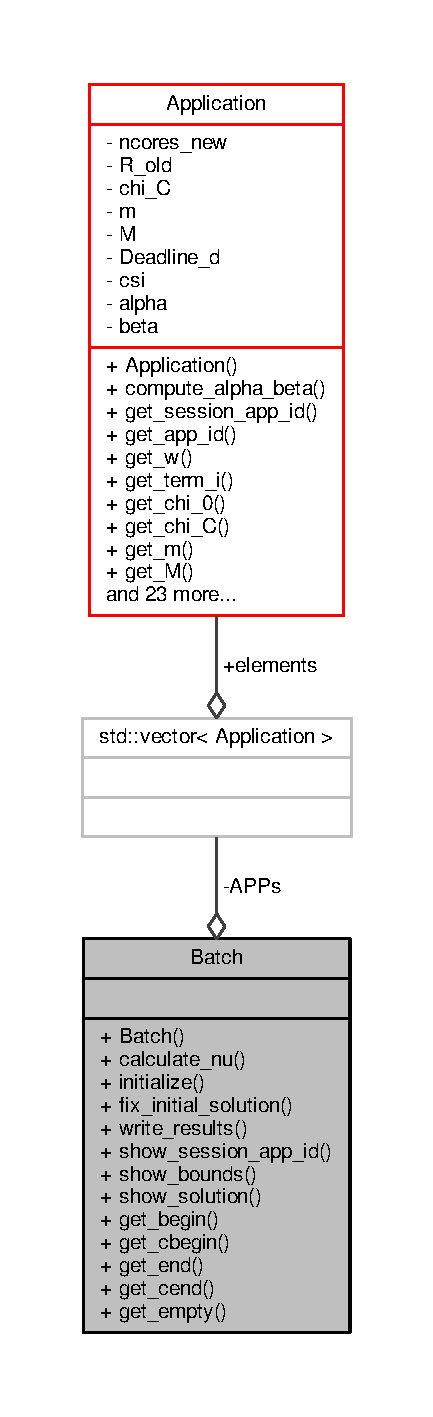
\includegraphics[width=309pt]{classBatch__coll__graph}
\end{center}
\end{figure}
\subsection*{Public Member Functions}
\begin{DoxyCompactItemize}
\item 
\hyperlink{classBatch_aea459d16c99c2f02af53b3ad5b0ff12d}{Batch} (std\-::vector$<$ \hyperlink{classApplication}{Application} $>$ apps)
\item 
void \hyperlink{classBatch_a14f132321413b45d6446200807451414}{calculate\-\_\-nu} (\hyperlink{classoptJrParameters}{opt\-Jr\-Parameters} \&par)
\item 
void \hyperlink{classBatch_ae212d22fa812b51160f57507242152c1}{initialize} (\hyperlink{readConfigurationFile_8hh_ab8f35b1da3261263c5e9c0e7c8921f5c}{s\-Configuration} \&configuration, M\-Y\-S\-Q\-L $\ast$conn, \hyperlink{classoptJrParameters}{opt\-Jr\-Parameters} \&par)
\item 
void \hyperlink{classBatch_ac50dad870490ca7c60e0e15d86c02614}{fix\-Initial\-Solution} (\hyperlink{classoptJrParameters}{opt\-Jr\-Parameters} \&par)
\item 
\hyperlink{candidates_8hh_af1ec7d668b0f7361dc7e1e1da5c4ce7d}{s\-Candidates} \hyperlink{classBatch_acf54e153a40b4720b1f7bebf000b1600}{approximated\-Loop} (int \&iteration, \hyperlink{classoptJrParameters}{opt\-Jr\-Parameters} \&par)
\end{DoxyCompactItemize}
\subsection*{Public Attributes}
\begin{DoxyCompactItemize}
\item 
std\-::vector$<$ \hyperlink{classApplication}{Application} $>$ \hyperlink{classBatch_a757bf1a36fee46b1b47263ab4a59c560}{A\-P\-Ps}
\end{DoxyCompactItemize}


\subsection{Constructor \& Destructor Documentation}
\hypertarget{classBatch_aea459d16c99c2f02af53b3ad5b0ff12d}{\index{Batch@{Batch}!Batch@{Batch}}
\index{Batch@{Batch}!Batch@{Batch}}
\subsubsection[{Batch}]{\setlength{\rightskip}{0pt plus 5cm}Batch\-::\-Batch (
\begin{DoxyParamCaption}
\item[{std\-::vector$<$ {\bf Application} $>$}]{apps}
\end{DoxyParamCaption}
)\hspace{0.3cm}{\ttfamily [inline]}}}\label{classBatch_aea459d16c99c2f02af53b3ad5b0ff12d}


\subsection{Member Function Documentation}
\hypertarget{classBatch_acf54e153a40b4720b1f7bebf000b1600}{\index{Batch@{Batch}!approximated\-Loop@{approximated\-Loop}}
\index{approximated\-Loop@{approximated\-Loop}!Batch@{Batch}}
\subsubsection[{approximated\-Loop}]{\setlength{\rightskip}{0pt plus 5cm}{\bf s\-Candidates} Batch\-::approximated\-Loop (
\begin{DoxyParamCaption}
\item[{int \&}]{iteration, }
\item[{{\bf opt\-Jr\-Parameters} \&}]{par}
\end{DoxyParamCaption}
)}}\label{classBatch_acf54e153a40b4720b1f7bebf000b1600}


Here is the call graph for this function\-:\nopagebreak
\begin{figure}[H]
\begin{center}
\leavevmode
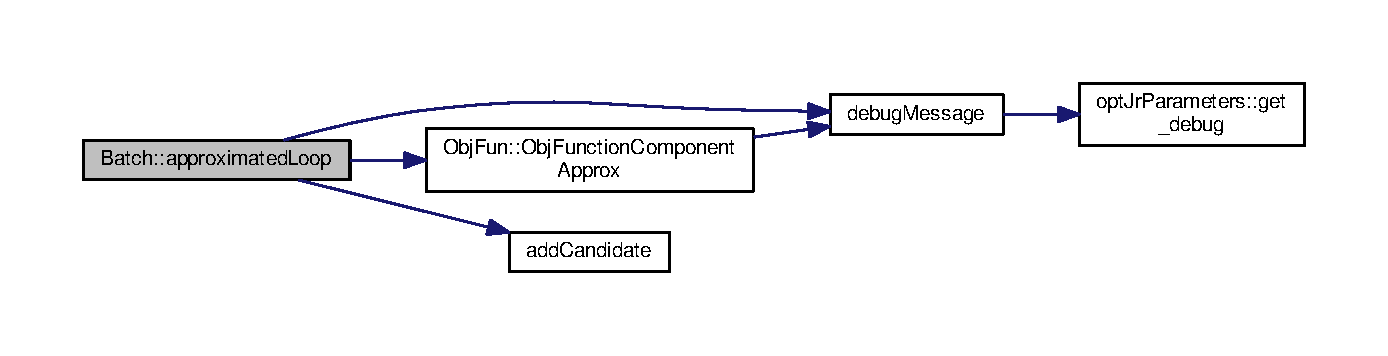
\includegraphics[width=350pt]{classBatch_acf54e153a40b4720b1f7bebf000b1600_cgraph}
\end{center}
\end{figure}




Here is the caller graph for this function\-:\nopagebreak
\begin{figure}[H]
\begin{center}
\leavevmode
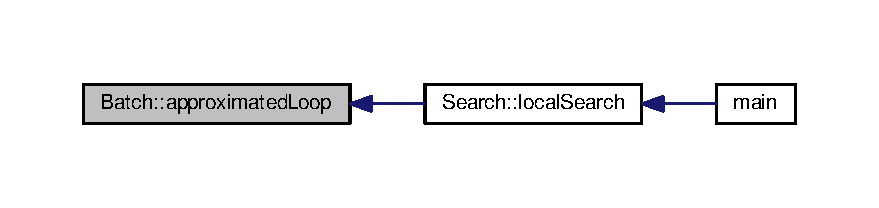
\includegraphics[width=350pt]{classBatch_acf54e153a40b4720b1f7bebf000b1600_icgraph}
\end{center}
\end{figure}


\hypertarget{classBatch_a14f132321413b45d6446200807451414}{\index{Batch@{Batch}!calculate\-\_\-nu@{calculate\-\_\-nu}}
\index{calculate\-\_\-nu@{calculate\-\_\-nu}!Batch@{Batch}}
\subsubsection[{calculate\-\_\-nu}]{\setlength{\rightskip}{0pt plus 5cm}void Batch\-::calculate\-\_\-nu (
\begin{DoxyParamCaption}
\item[{{\bf opt\-Jr\-Parameters} \&}]{par}
\end{DoxyParamCaption}
)}}\label{classBatch_a14f132321413b45d6446200807451414}


Here is the call graph for this function\-:\nopagebreak
\begin{figure}[H]
\begin{center}
\leavevmode
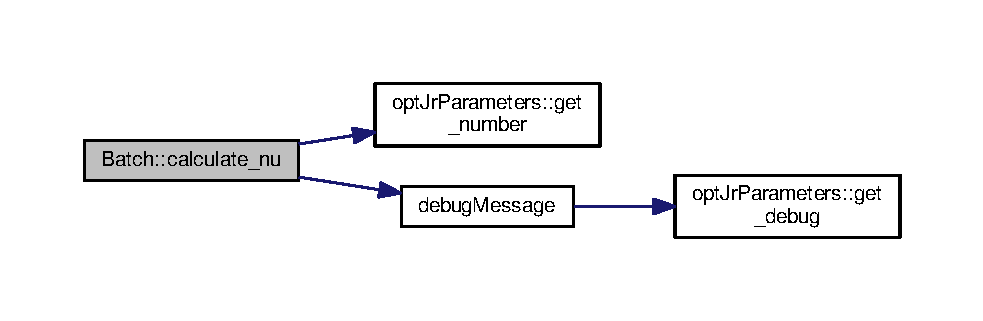
\includegraphics[width=350pt]{classBatch_a14f132321413b45d6446200807451414_cgraph}
\end{center}
\end{figure}




Here is the caller graph for this function\-:\nopagebreak
\begin{figure}[H]
\begin{center}
\leavevmode
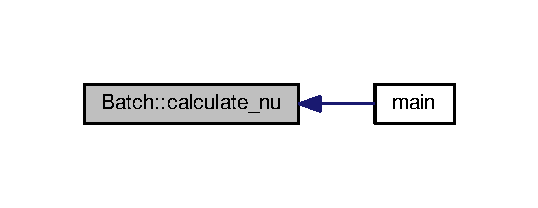
\includegraphics[width=258pt]{classBatch_a14f132321413b45d6446200807451414_icgraph}
\end{center}
\end{figure}


\hypertarget{classBatch_ac50dad870490ca7c60e0e15d86c02614}{\index{Batch@{Batch}!fix\-Initial\-Solution@{fix\-Initial\-Solution}}
\index{fix\-Initial\-Solution@{fix\-Initial\-Solution}!Batch@{Batch}}
\subsubsection[{fix\-Initial\-Solution}]{\setlength{\rightskip}{0pt plus 5cm}void Batch\-::fix\-Initial\-Solution (
\begin{DoxyParamCaption}
\item[{{\bf opt\-Jr\-Parameters} \&}]{par}
\end{DoxyParamCaption}
)}}\label{classBatch_ac50dad870490ca7c60e0e15d86c02614}


Here is the call graph for this function\-:\nopagebreak
\begin{figure}[H]
\begin{center}
\leavevmode
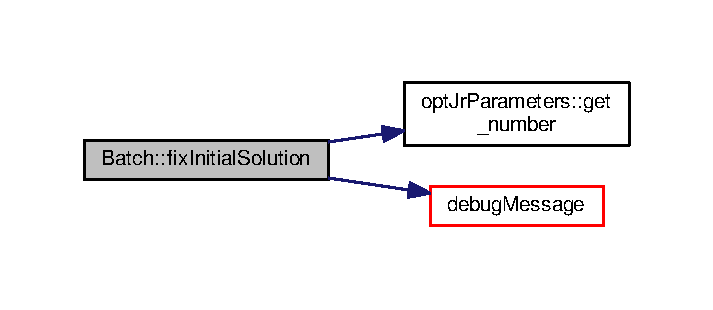
\includegraphics[width=350pt]{classBatch_ac50dad870490ca7c60e0e15d86c02614_cgraph}
\end{center}
\end{figure}




Here is the caller graph for this function\-:\nopagebreak
\begin{figure}[H]
\begin{center}
\leavevmode
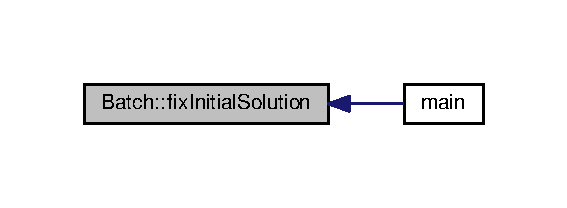
\includegraphics[width=272pt]{classBatch_ac50dad870490ca7c60e0e15d86c02614_icgraph}
\end{center}
\end{figure}


\hypertarget{classBatch_ae212d22fa812b51160f57507242152c1}{\index{Batch@{Batch}!initialize@{initialize}}
\index{initialize@{initialize}!Batch@{Batch}}
\subsubsection[{initialize}]{\setlength{\rightskip}{0pt plus 5cm}void Batch\-::initialize (
\begin{DoxyParamCaption}
\item[{{\bf s\-Configuration} \&}]{configuration, }
\item[{M\-Y\-S\-Q\-L $\ast$}]{conn, }
\item[{{\bf opt\-Jr\-Parameters} \&}]{par}
\end{DoxyParamCaption}
)}}\label{classBatch_ae212d22fa812b51160f57507242152c1}


Here is the call graph for this function\-:\nopagebreak
\begin{figure}[H]
\begin{center}
\leavevmode
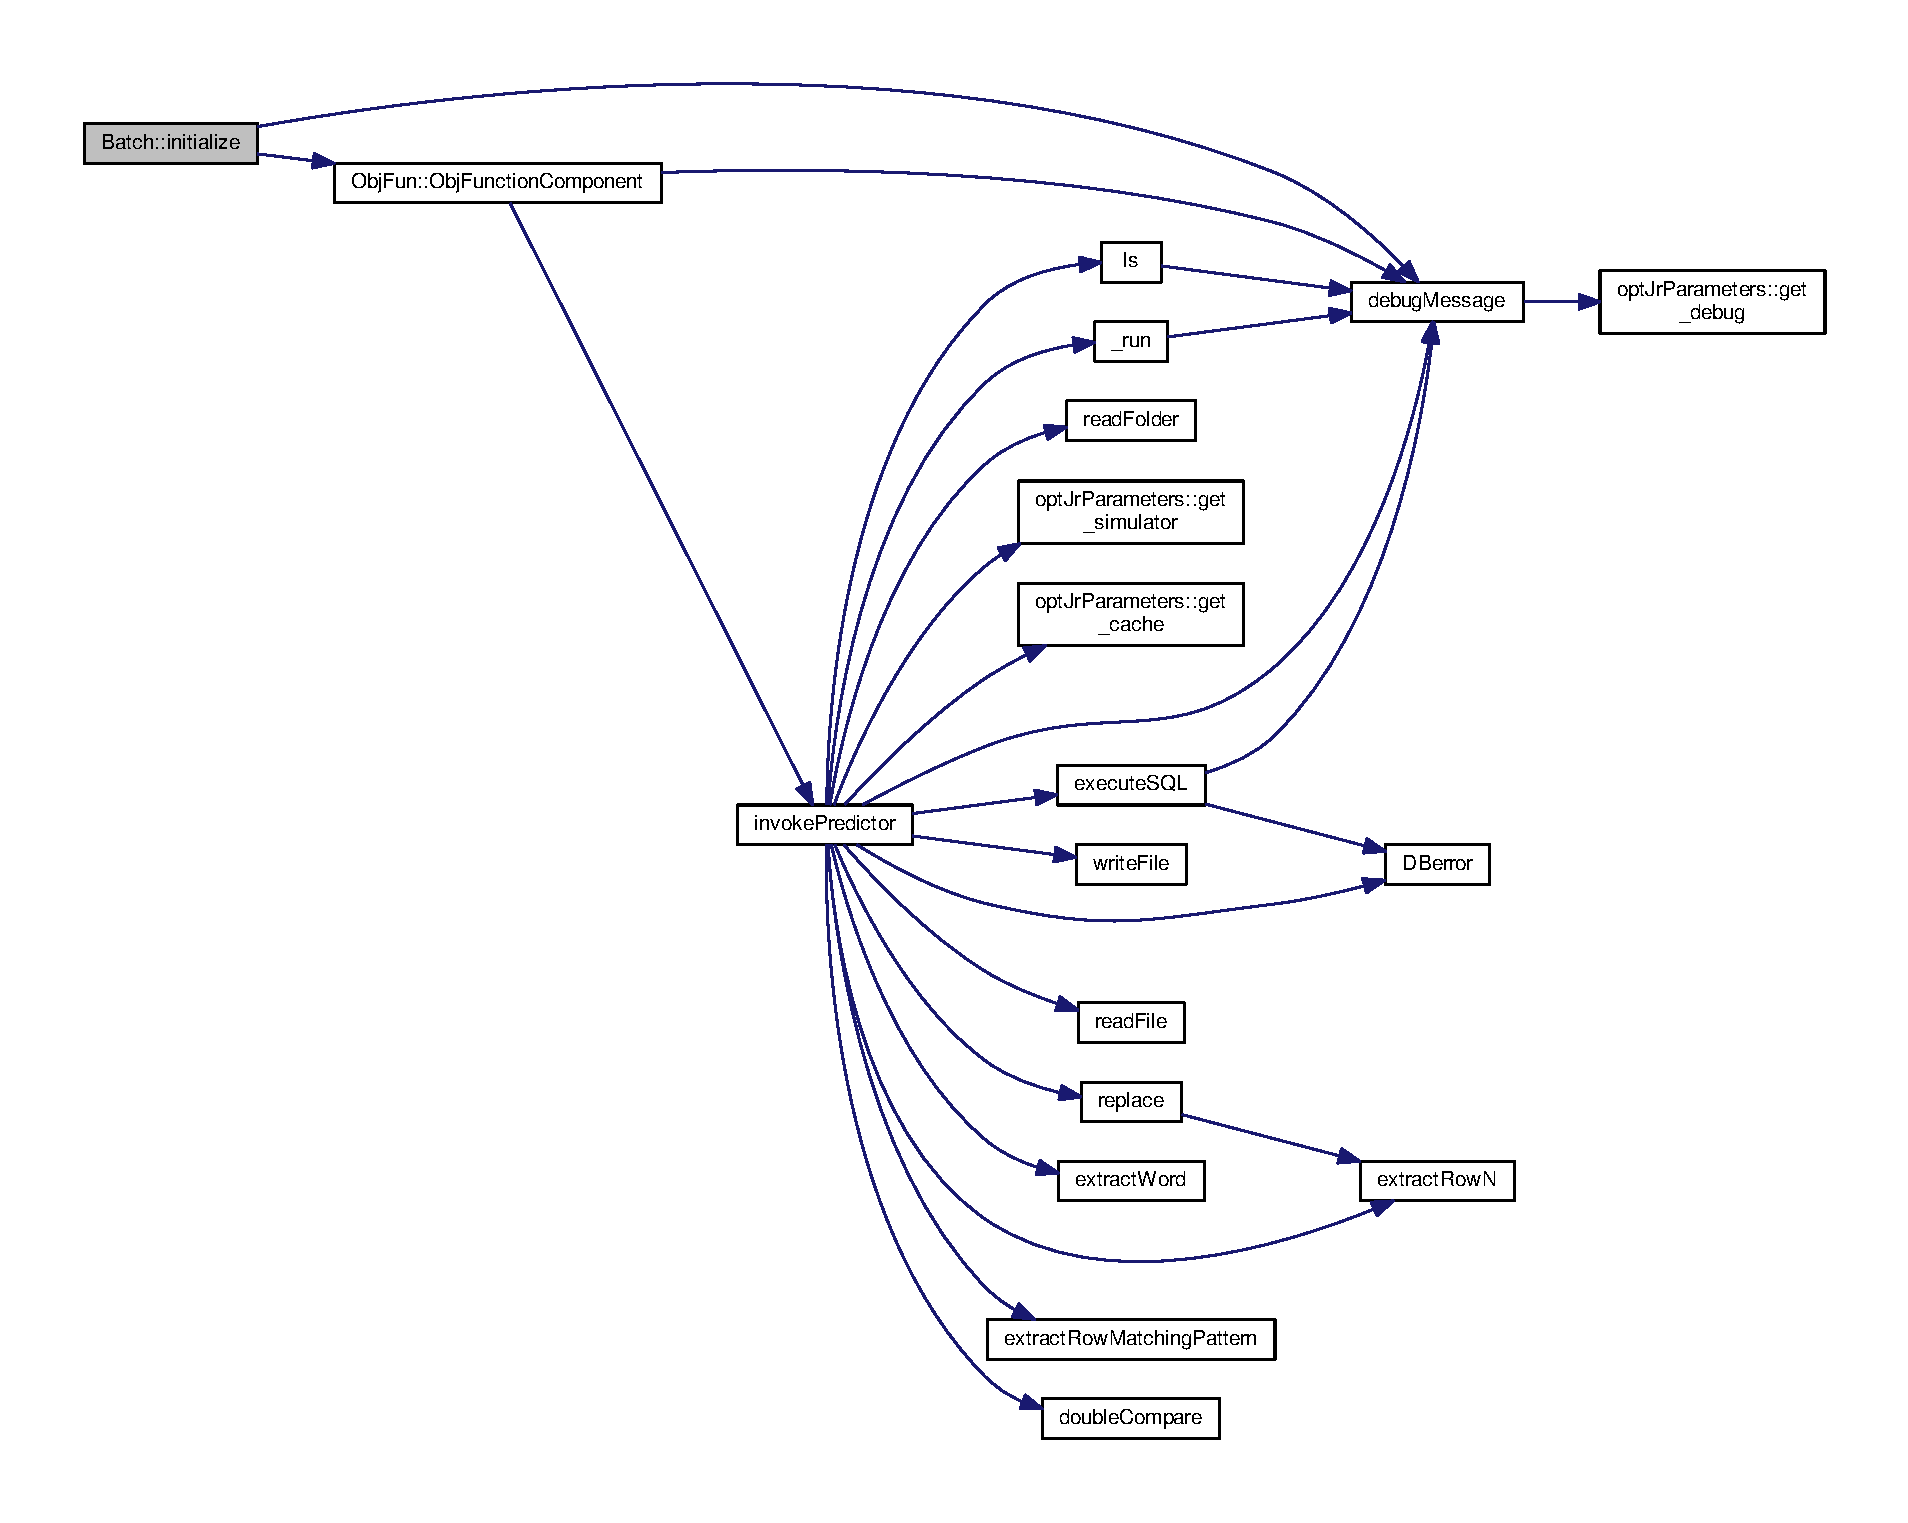
\includegraphics[width=350pt]{classBatch_ae212d22fa812b51160f57507242152c1_cgraph}
\end{center}
\end{figure}




Here is the caller graph for this function\-:\nopagebreak
\begin{figure}[H]
\begin{center}
\leavevmode
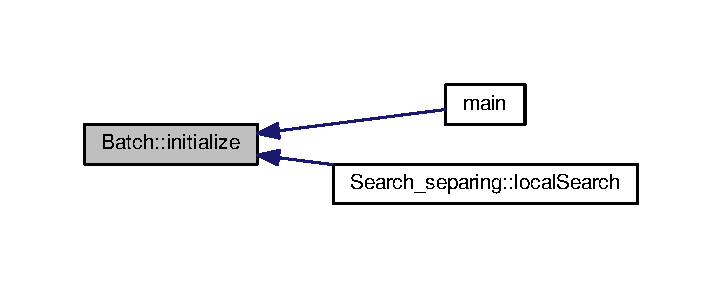
\includegraphics[width=238pt]{classBatch_ae212d22fa812b51160f57507242152c1_icgraph}
\end{center}
\end{figure}




\subsection{Member Data Documentation}
\hypertarget{classBatch_a757bf1a36fee46b1b47263ab4a59c560}{\index{Batch@{Batch}!A\-P\-Ps@{A\-P\-Ps}}
\index{A\-P\-Ps@{A\-P\-Ps}!Batch@{Batch}}
\subsubsection[{A\-P\-Ps}]{\setlength{\rightskip}{0pt plus 5cm}std\-::vector$<${\bf Application}$>$ Batch\-::\-A\-P\-Ps}}\label{classBatch_a757bf1a36fee46b1b47263ab4a59c560}


The documentation for this class was generated from the following files\-:\begin{DoxyCompactItemize}
\item 
/vagrant/\-P\-R\-O\-J\-E\-C\-T\-\_\-\-S\-P\-A\-R\-K/\-P\-A\-C\-S\-\_\-\-P\-R\-O\-J\-E\-C\-T/opt\-\_\-jr/src/\hyperlink{batch_8hh}{batch.\-hh}\item 
/vagrant/\-P\-R\-O\-J\-E\-C\-T\-\_\-\-S\-P\-A\-R\-K/\-P\-A\-C\-S\-\_\-\-P\-R\-O\-J\-E\-C\-T/opt\-\_\-jr/src/\hyperlink{batch_8cpp}{batch.\-cpp}\end{DoxyCompactItemize}

\hypertarget{classBounds}{\section{Bounds Class Reference}
\label{classBounds}\index{Bounds@{Bounds}}
}


{\ttfamily \#include $<$bounds.\-hh$>$}



Collaboration diagram for Bounds\-:
\nopagebreak
\begin{figure}[H]
\begin{center}
\leavevmode
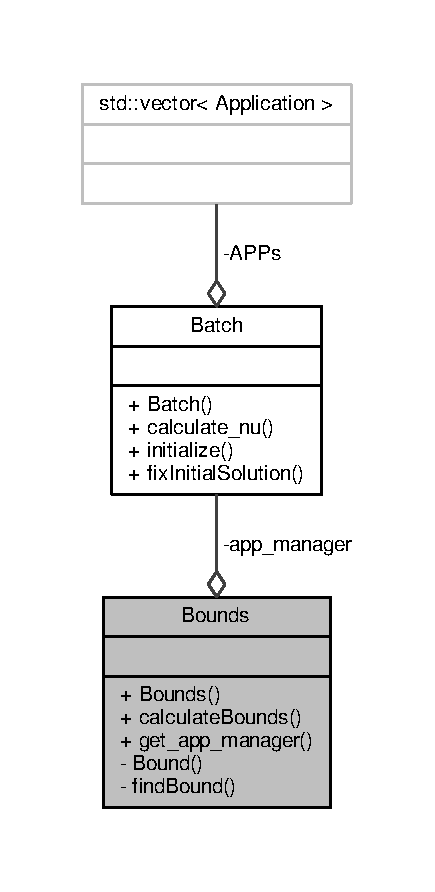
\includegraphics[width=209pt]{classBounds__coll__graph}
\end{center}
\end{figure}
\subsection*{Public Member Functions}
\begin{DoxyCompactItemize}
\item 
\hyperlink{classBounds_a57a9894ee450eb885a83e884b5fb79e7}{Bounds} (\hyperlink{classBatch}{Batch} app\-\_\-m)
\item 
void \hyperlink{classBounds_aefc7e0bd2cd1c5850a903aabe0351dbe}{calculate\-Bounds} (\hyperlink{readConfigurationFile_8hh_ab8f35b1da3261263c5e9c0e7c8921f5c}{s\-Configuration} \&configuration, M\-Y\-S\-Q\-L $\ast$conn, \hyperlink{classoptJrParameters}{opt\-Jr\-Parameters} \&par)
\item 
\hyperlink{classBatch}{Batch} \hyperlink{classBounds_aefebbfe17ca3a7d6a0f6cbf4a0bf2782}{get\-\_\-app\-\_\-manager} ()
\end{DoxyCompactItemize}
\subsection*{Private Member Functions}
\begin{DoxyCompactItemize}
\item 
void \hyperlink{classBounds_a6bc038892059a8181984daff0003065f}{Bound} (\hyperlink{readConfigurationFile_8hh_ab8f35b1da3261263c5e9c0e7c8921f5c}{s\-Configuration} \&configuration, M\-Y\-S\-Q\-L $\ast$conn, \hyperlink{classApplication}{Application} \&app, \hyperlink{classoptJrParameters}{opt\-Jr\-Parameters} \&par, int flag\-Dagsim)
\item 
void \hyperlink{classBounds_ade8356aa22e675868ba98226e4216cf3}{find\-Bound} (\hyperlink{readConfigurationFile_8hh_ab8f35b1da3261263c5e9c0e7c8921f5c}{s\-Configuration} \&configuration, M\-Y\-S\-Q\-L $\ast$conn, char $\ast$db, \hyperlink{classApplication}{Application} \&app, \hyperlink{classoptJrParameters}{opt\-Jr\-Parameters} \&par)
\end{DoxyCompactItemize}
\subsection*{Private Attributes}
\begin{DoxyCompactItemize}
\item 
\hyperlink{classBatch}{Batch} \hyperlink{classBounds_a9b463c00e877b6bf67d9e1ff4f36950b}{app\-\_\-manager}
\end{DoxyCompactItemize}


\subsection{Detailed Description}
\hyperlink{classBounds}{Bounds} class provide a method to evaluate the bound for the applications in B\-A\-T\-C\-H i.\-e. the minimal number of cores necessary to finish the execution before the deadline 

\subsection{Constructor \& Destructor Documentation}
\hypertarget{classBounds_a57a9894ee450eb885a83e884b5fb79e7}{\index{Bounds@{Bounds}!Bounds@{Bounds}}
\index{Bounds@{Bounds}!Bounds@{Bounds}}
\subsubsection[{Bounds}]{\setlength{\rightskip}{0pt plus 5cm}Bounds\-::\-Bounds (
\begin{DoxyParamCaption}
\item[{{\bf Batch}}]{app\-\_\-m}
\end{DoxyParamCaption}
)\hspace{0.3cm}{\ttfamily [inline]}}}\label{classBounds_a57a9894ee450eb885a83e884b5fb79e7}


\subsection{Member Function Documentation}
\hypertarget{classBounds_a6bc038892059a8181984daff0003065f}{\index{Bounds@{Bounds}!Bound@{Bound}}
\index{Bound@{Bound}!Bounds@{Bounds}}
\subsubsection[{Bound}]{\setlength{\rightskip}{0pt plus 5cm}void Bounds\-::\-Bound (
\begin{DoxyParamCaption}
\item[{{\bf s\-Configuration} \&}]{configuration, }
\item[{M\-Y\-S\-Q\-L $\ast$}]{conn, }
\item[{{\bf Application} \&}]{app, }
\item[{{\bf opt\-Jr\-Parameters} \&}]{par, }
\item[{int}]{flag\-Dagsim}
\end{DoxyParamCaption}
)\hspace{0.3cm}{\ttfamily [private]}}}\label{classBounds_a6bc038892059a8181984daff0003065f}


Here is the caller graph for this function\-:\nopagebreak
\begin{figure}[H]
\begin{center}
\leavevmode
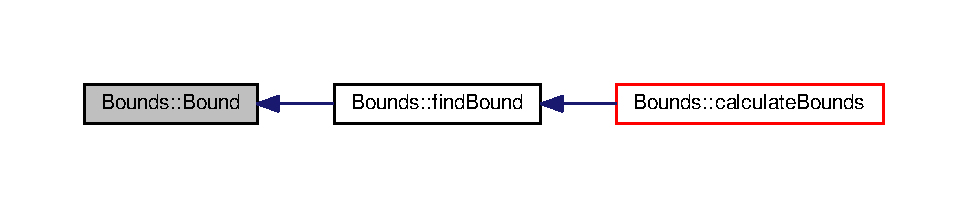
\includegraphics[width=350pt]{classBounds_a6bc038892059a8181984daff0003065f_icgraph}
\end{center}
\end{figure}


\hypertarget{classBounds_aefc7e0bd2cd1c5850a903aabe0351dbe}{\index{Bounds@{Bounds}!calculate\-Bounds@{calculate\-Bounds}}
\index{calculate\-Bounds@{calculate\-Bounds}!Bounds@{Bounds}}
\subsubsection[{calculate\-Bounds}]{\setlength{\rightskip}{0pt plus 5cm}void Bounds\-::calculate\-Bounds (
\begin{DoxyParamCaption}
\item[{{\bf s\-Configuration} \&}]{configuration, }
\item[{M\-Y\-S\-Q\-L $\ast$}]{conn, }
\item[{{\bf opt\-Jr\-Parameters} \&}]{par}
\end{DoxyParamCaption}
)}}\label{classBounds_aefc7e0bd2cd1c5850a903aabe0351dbe}
calculate\-Bounds evaluates the bound for the applications in B\-A\-T\-C\-H i.\-e. the minimal number of cores necessary to finish the execution before the deadline. The function looks before if the result is already stored in the database, otherwise it invokes the predictor doing a \char`\"{}\-H\-I\-L\-L C\-L\-I\-M\-B\-I\-N\-G\char`\"{}. If the number of threads in the configuration file is greater than 0, it does the computations in parallel (using open\-M\-P). 

Here is the caller graph for this function\-:\nopagebreak
\begin{figure}[H]
\begin{center}
\leavevmode
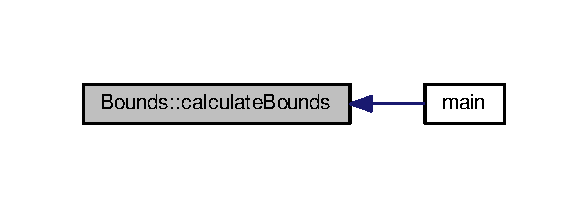
\includegraphics[width=282pt]{classBounds_aefc7e0bd2cd1c5850a903aabe0351dbe_icgraph}
\end{center}
\end{figure}


\hypertarget{classBounds_ade8356aa22e675868ba98226e4216cf3}{\index{Bounds@{Bounds}!find\-Bound@{find\-Bound}}
\index{find\-Bound@{find\-Bound}!Bounds@{Bounds}}
\subsubsection[{find\-Bound}]{\setlength{\rightskip}{0pt plus 5cm}void Bounds\-::find\-Bound (
\begin{DoxyParamCaption}
\item[{{\bf s\-Configuration} \&}]{configuration, }
\item[{M\-Y\-S\-Q\-L $\ast$}]{conn, }
\item[{char $\ast$}]{db, }
\item[{{\bf Application} \&}]{app, }
\item[{{\bf opt\-Jr\-Parameters} \&}]{par}
\end{DoxyParamCaption}
)\hspace{0.3cm}{\ttfamily [private]}}}\label{classBounds_ade8356aa22e675868ba98226e4216cf3}


Here is the caller graph for this function\-:\nopagebreak
\begin{figure}[H]
\begin{center}
\leavevmode
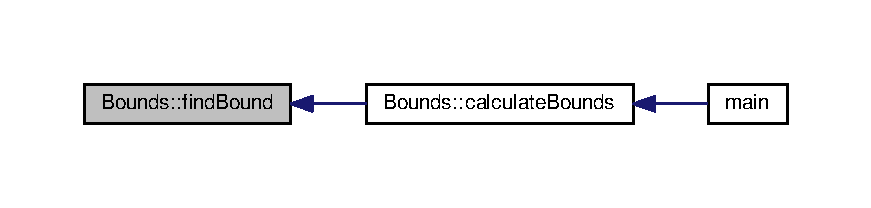
\includegraphics[width=350pt]{classBounds_ade8356aa22e675868ba98226e4216cf3_icgraph}
\end{center}
\end{figure}


\hypertarget{classBounds_aefebbfe17ca3a7d6a0f6cbf4a0bf2782}{\index{Bounds@{Bounds}!get\-\_\-app\-\_\-manager@{get\-\_\-app\-\_\-manager}}
\index{get\-\_\-app\-\_\-manager@{get\-\_\-app\-\_\-manager}!Bounds@{Bounds}}
\subsubsection[{get\-\_\-app\-\_\-manager}]{\setlength{\rightskip}{0pt plus 5cm}{\bf Batch} Bounds\-::get\-\_\-app\-\_\-manager (
\begin{DoxyParamCaption}
{}
\end{DoxyParamCaption}
)\hspace{0.3cm}{\ttfamily [inline]}}}\label{classBounds_aefebbfe17ca3a7d6a0f6cbf4a0bf2782}


Here is the caller graph for this function\-:\nopagebreak
\begin{figure}[H]
\begin{center}
\leavevmode
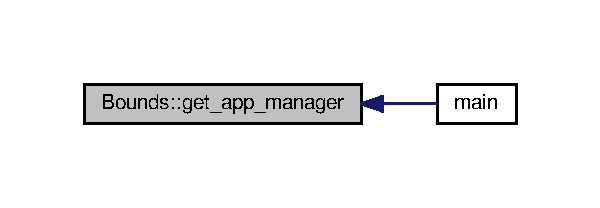
\includegraphics[width=288pt]{classBounds_aefebbfe17ca3a7d6a0f6cbf4a0bf2782_icgraph}
\end{center}
\end{figure}




\subsection{Member Data Documentation}
\hypertarget{classBounds_a9b463c00e877b6bf67d9e1ff4f36950b}{\index{Bounds@{Bounds}!app\-\_\-manager@{app\-\_\-manager}}
\index{app\-\_\-manager@{app\-\_\-manager}!Bounds@{Bounds}}
\subsubsection[{app\-\_\-manager}]{\setlength{\rightskip}{0pt plus 5cm}{\bf Batch} Bounds\-::app\-\_\-manager\hspace{0.3cm}{\ttfamily [private]}}}\label{classBounds_a9b463c00e877b6bf67d9e1ff4f36950b}


The documentation for this class was generated from the following files\-:\begin{DoxyCompactItemize}
\item 
/vagrant/\-P\-R\-O\-J\-E\-C\-T\-\_\-\-S\-P\-A\-R\-K/\-P\-A\-C\-S\-\_\-\-P\-R\-O\-J\-E\-C\-T/opt\-\_\-jr/src/\hyperlink{bounds_8hh}{bounds.\-hh}\item 
/vagrant/\-P\-R\-O\-J\-E\-C\-T\-\_\-\-S\-P\-A\-R\-K/\-P\-A\-C\-S\-\_\-\-P\-R\-O\-J\-E\-C\-T/opt\-\_\-jr/src/\hyperlink{bounds_8cpp}{bounds.\-cpp}\end{DoxyCompactItemize}

\hypertarget{classCandidate}{\section{Candidate Class Reference}
\label{classCandidate}\index{Candidate@{Candidate}}
}


{\ttfamily \#include $<$candidates.\-hh$>$}



Collaboration diagram for Candidate\-:\nopagebreak
\begin{figure}[H]
\begin{center}
\leavevmode
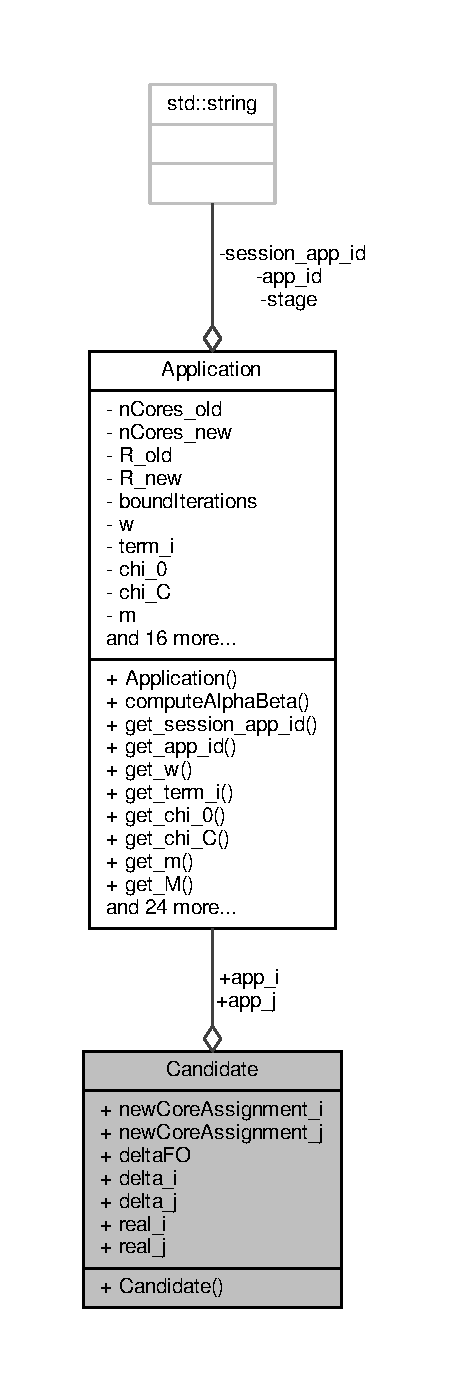
\includegraphics[width=309pt]{classCandidate__coll__graph}
\end{center}
\end{figure}
\subsection*{Public Member Functions}
\begin{DoxyCompactItemize}
\item 
\hyperlink{classCandidate_a2d1453a6b8c1a39561e67a2c67b79ed1}{Candidate} (\hyperlink{classApplication}{Application} $\ast$i, \hyperlink{classApplication}{Application} $\ast$j, int N\-Ci, int N\-Cj, double D\-\_\-\-F\-O, int d\-\_\-i, int d\-\_\-j)
\end{DoxyCompactItemize}
\subsection*{Public Attributes}
\begin{DoxyCompactItemize}
\item 
\hyperlink{classApplication}{Application} $\ast$ \hyperlink{classCandidate_a1bfed0429bba41f57dce0fbd37225c2c}{app\-\_\-i}
\item 
int \hyperlink{classCandidate_a859313416296683b7c0496d842dab48a}{new\-Core\-Assignment\-\_\-i}
\item 
int \hyperlink{classCandidate_ab1033e1f3e0060f0773c7d9268c2ce0b}{delta\-\_\-i}
\item 
double \hyperlink{classCandidate_a93a050a3128d98f446176d9411535eea}{real\-\_\-i}
\item 
\hyperlink{classApplication}{Application} $\ast$ \hyperlink{classCandidate_a8b0f26e8b45e9a3331be8a9694d3be5e}{app\-\_\-j}
\item 
int \hyperlink{classCandidate_a1203966358bd849169b5f967de3c2bf7}{new\-Core\-Assignment\-\_\-j}
\item 
int \hyperlink{classCandidate_a02528143e2448bfcad797aae2fe1ac90}{delta\-\_\-j}
\item 
double \hyperlink{classCandidate_ad7e4bca76815c11f378f005baa93bffb}{real\-\_\-j}
\item 
int \hyperlink{classCandidate_a7136b28b9f4ef84a661ba4132f59eaa3}{nodes\-\_\-i}
\item 
int \hyperlink{classCandidate_affe483f905741a62769d1fbebae48b4e}{nodes\-\_\-j}
\item 
double \hyperlink{classCandidate_a1bfc07aae3b3914bba57e057936399e7}{delta\-F\-O}
\end{DoxyCompactItemize}


\subsection{Constructor \& Destructor Documentation}
\hypertarget{classCandidate_a2d1453a6b8c1a39561e67a2c67b79ed1}{\index{Candidate@{Candidate}!Candidate@{Candidate}}
\index{Candidate@{Candidate}!Candidate@{Candidate}}
\subsubsection[{Candidate}]{\setlength{\rightskip}{0pt plus 5cm}Candidate\-::\-Candidate (
\begin{DoxyParamCaption}
\item[{{\bf Application} $\ast$}]{i, }
\item[{{\bf Application} $\ast$}]{j, }
\item[{int}]{N\-Ci, }
\item[{int}]{N\-Cj, }
\item[{double}]{D\-\_\-\-F\-O, }
\item[{int}]{d\-\_\-i, }
\item[{int}]{d\-\_\-j}
\end{DoxyParamCaption}
)\hspace{0.3cm}{\ttfamily [inline]}}}\label{classCandidate_a2d1453a6b8c1a39561e67a2c67b79ed1}


\subsection{Member Data Documentation}
\hypertarget{classCandidate_a1bfed0429bba41f57dce0fbd37225c2c}{\index{Candidate@{Candidate}!app\-\_\-i@{app\-\_\-i}}
\index{app\-\_\-i@{app\-\_\-i}!Candidate@{Candidate}}
\subsubsection[{app\-\_\-i}]{\setlength{\rightskip}{0pt plus 5cm}{\bf Application}$\ast$ Candidate\-::app\-\_\-i}}\label{classCandidate_a1bfed0429bba41f57dce0fbd37225c2c}
\hypertarget{classCandidate_a8b0f26e8b45e9a3331be8a9694d3be5e}{\index{Candidate@{Candidate}!app\-\_\-j@{app\-\_\-j}}
\index{app\-\_\-j@{app\-\_\-j}!Candidate@{Candidate}}
\subsubsection[{app\-\_\-j}]{\setlength{\rightskip}{0pt plus 5cm}{\bf Application}$\ast$ Candidate\-::app\-\_\-j}}\label{classCandidate_a8b0f26e8b45e9a3331be8a9694d3be5e}
\hypertarget{classCandidate_ab1033e1f3e0060f0773c7d9268c2ce0b}{\index{Candidate@{Candidate}!delta\-\_\-i@{delta\-\_\-i}}
\index{delta\-\_\-i@{delta\-\_\-i}!Candidate@{Candidate}}
\subsubsection[{delta\-\_\-i}]{\setlength{\rightskip}{0pt plus 5cm}int Candidate\-::delta\-\_\-i}}\label{classCandidate_ab1033e1f3e0060f0773c7d9268c2ce0b}
\hypertarget{classCandidate_a02528143e2448bfcad797aae2fe1ac90}{\index{Candidate@{Candidate}!delta\-\_\-j@{delta\-\_\-j}}
\index{delta\-\_\-j@{delta\-\_\-j}!Candidate@{Candidate}}
\subsubsection[{delta\-\_\-j}]{\setlength{\rightskip}{0pt plus 5cm}int Candidate\-::delta\-\_\-j}}\label{classCandidate_a02528143e2448bfcad797aae2fe1ac90}
\hypertarget{classCandidate_a1bfc07aae3b3914bba57e057936399e7}{\index{Candidate@{Candidate}!delta\-F\-O@{delta\-F\-O}}
\index{delta\-F\-O@{delta\-F\-O}!Candidate@{Candidate}}
\subsubsection[{delta\-F\-O}]{\setlength{\rightskip}{0pt plus 5cm}double Candidate\-::delta\-F\-O}}\label{classCandidate_a1bfc07aae3b3914bba57e057936399e7}
\hypertarget{classCandidate_a859313416296683b7c0496d842dab48a}{\index{Candidate@{Candidate}!new\-Core\-Assignment\-\_\-i@{new\-Core\-Assignment\-\_\-i}}
\index{new\-Core\-Assignment\-\_\-i@{new\-Core\-Assignment\-\_\-i}!Candidate@{Candidate}}
\subsubsection[{new\-Core\-Assignment\-\_\-i}]{\setlength{\rightskip}{0pt plus 5cm}int Candidate\-::new\-Core\-Assignment\-\_\-i}}\label{classCandidate_a859313416296683b7c0496d842dab48a}
\hypertarget{classCandidate_a1203966358bd849169b5f967de3c2bf7}{\index{Candidate@{Candidate}!new\-Core\-Assignment\-\_\-j@{new\-Core\-Assignment\-\_\-j}}
\index{new\-Core\-Assignment\-\_\-j@{new\-Core\-Assignment\-\_\-j}!Candidate@{Candidate}}
\subsubsection[{new\-Core\-Assignment\-\_\-j}]{\setlength{\rightskip}{0pt plus 5cm}int Candidate\-::new\-Core\-Assignment\-\_\-j}}\label{classCandidate_a1203966358bd849169b5f967de3c2bf7}
\hypertarget{classCandidate_a7136b28b9f4ef84a661ba4132f59eaa3}{\index{Candidate@{Candidate}!nodes\-\_\-i@{nodes\-\_\-i}}
\index{nodes\-\_\-i@{nodes\-\_\-i}!Candidate@{Candidate}}
\subsubsection[{nodes\-\_\-i}]{\setlength{\rightskip}{0pt plus 5cm}int Candidate\-::nodes\-\_\-i}}\label{classCandidate_a7136b28b9f4ef84a661ba4132f59eaa3}
\hypertarget{classCandidate_affe483f905741a62769d1fbebae48b4e}{\index{Candidate@{Candidate}!nodes\-\_\-j@{nodes\-\_\-j}}
\index{nodes\-\_\-j@{nodes\-\_\-j}!Candidate@{Candidate}}
\subsubsection[{nodes\-\_\-j}]{\setlength{\rightskip}{0pt plus 5cm}int Candidate\-::nodes\-\_\-j}}\label{classCandidate_affe483f905741a62769d1fbebae48b4e}
\hypertarget{classCandidate_a93a050a3128d98f446176d9411535eea}{\index{Candidate@{Candidate}!real\-\_\-i@{real\-\_\-i}}
\index{real\-\_\-i@{real\-\_\-i}!Candidate@{Candidate}}
\subsubsection[{real\-\_\-i}]{\setlength{\rightskip}{0pt plus 5cm}double Candidate\-::real\-\_\-i}}\label{classCandidate_a93a050a3128d98f446176d9411535eea}
\hypertarget{classCandidate_ad7e4bca76815c11f378f005baa93bffb}{\index{Candidate@{Candidate}!real\-\_\-j@{real\-\_\-j}}
\index{real\-\_\-j@{real\-\_\-j}!Candidate@{Candidate}}
\subsubsection[{real\-\_\-j}]{\setlength{\rightskip}{0pt plus 5cm}double Candidate\-::real\-\_\-j}}\label{classCandidate_ad7e4bca76815c11f378f005baa93bffb}


The documentation for this class was generated from the following file\-:\begin{DoxyCompactItemize}
\item 
/vagrant/\-P\-R\-O\-J\-E\-C\-T\-\_\-\-S\-P\-A\-R\-K/\-P\-A\-C\-S\-\_\-\-P\-R\-O\-J\-E\-C\-T/opt\-\_\-jr/src/\hyperlink{candidates_8hh}{candidates.\-hh}\end{DoxyCompactItemize}

\hypertarget{classObjFun}{\section{Obj\-Fun Class Reference}
\label{classObjFun}\index{Obj\-Fun@{Obj\-Fun}}
}


{\ttfamily \#include $<$objective\-Function.\-hh$>$}

\subsection*{Static Public Member Functions}
\begin{DoxyCompactItemize}
\item 
static double \hyperlink{classObjFun_a7c9ecaa07ca776eb64f6e73f84513bc7}{Obj\-Function\-Component} (\hyperlink{readConfigurationFile_8hh_ab8f35b1da3261263c5e9c0e7c8921f5c}{s\-Configuration} \&configuration, M\-Y\-S\-Q\-L $\ast$conn, \hyperlink{classApplication}{Application} \&app, \hyperlink{classoptJrParameters}{opt\-Jr\-Parameters} \&par)
\item 
static double \hyperlink{classObjFun_abb89a994d34b44ec4cb6e0e2562c0107}{Obj\-Function\-Component\-Approx} (\hyperlink{classApplication}{Application} \&App, \hyperlink{classoptJrParameters}{opt\-Jr\-Parameters} \&par)
\item 
static double \hyperlink{classObjFun_ab36af3a1d85dbcaa79dc9b582b00928b}{Obj\-Function\-Global} (\hyperlink{readConfigurationFile_8hh_ab8f35b1da3261263c5e9c0e7c8921f5c}{s\-Configuration} \&configuration, M\-Y\-S\-Q\-L $\ast$conn, \hyperlink{classBatch}{Batch} \&App\-\_\-manager, \hyperlink{classoptJrParameters}{opt\-Jr\-Parameters} \&par)
\end{DoxyCompactItemize}


\subsection{Member Function Documentation}
\hypertarget{classObjFun_a7c9ecaa07ca776eb64f6e73f84513bc7}{\index{Obj\-Fun@{Obj\-Fun}!Obj\-Function\-Component@{Obj\-Function\-Component}}
\index{Obj\-Function\-Component@{Obj\-Function\-Component}!ObjFun@{Obj\-Fun}}
\subsubsection[{Obj\-Function\-Component}]{\setlength{\rightskip}{0pt plus 5cm}double Obj\-Fun\-::\-Obj\-Function\-Component (
\begin{DoxyParamCaption}
\item[{{\bf s\-Configuration} \&}]{configuration, }
\item[{M\-Y\-S\-Q\-L $\ast$}]{conn, }
\item[{{\bf Application} \&}]{app, }
\item[{{\bf opt\-Jr\-Parameters} \&}]{par}
\end{DoxyParamCaption}
)\hspace{0.3cm}{\ttfamily [static]}}}\label{classObjFun_a7c9ecaa07ca776eb64f6e73f84513bc7}


Here is the call graph for this function\-:\nopagebreak
\begin{figure}[H]
\begin{center}
\leavevmode
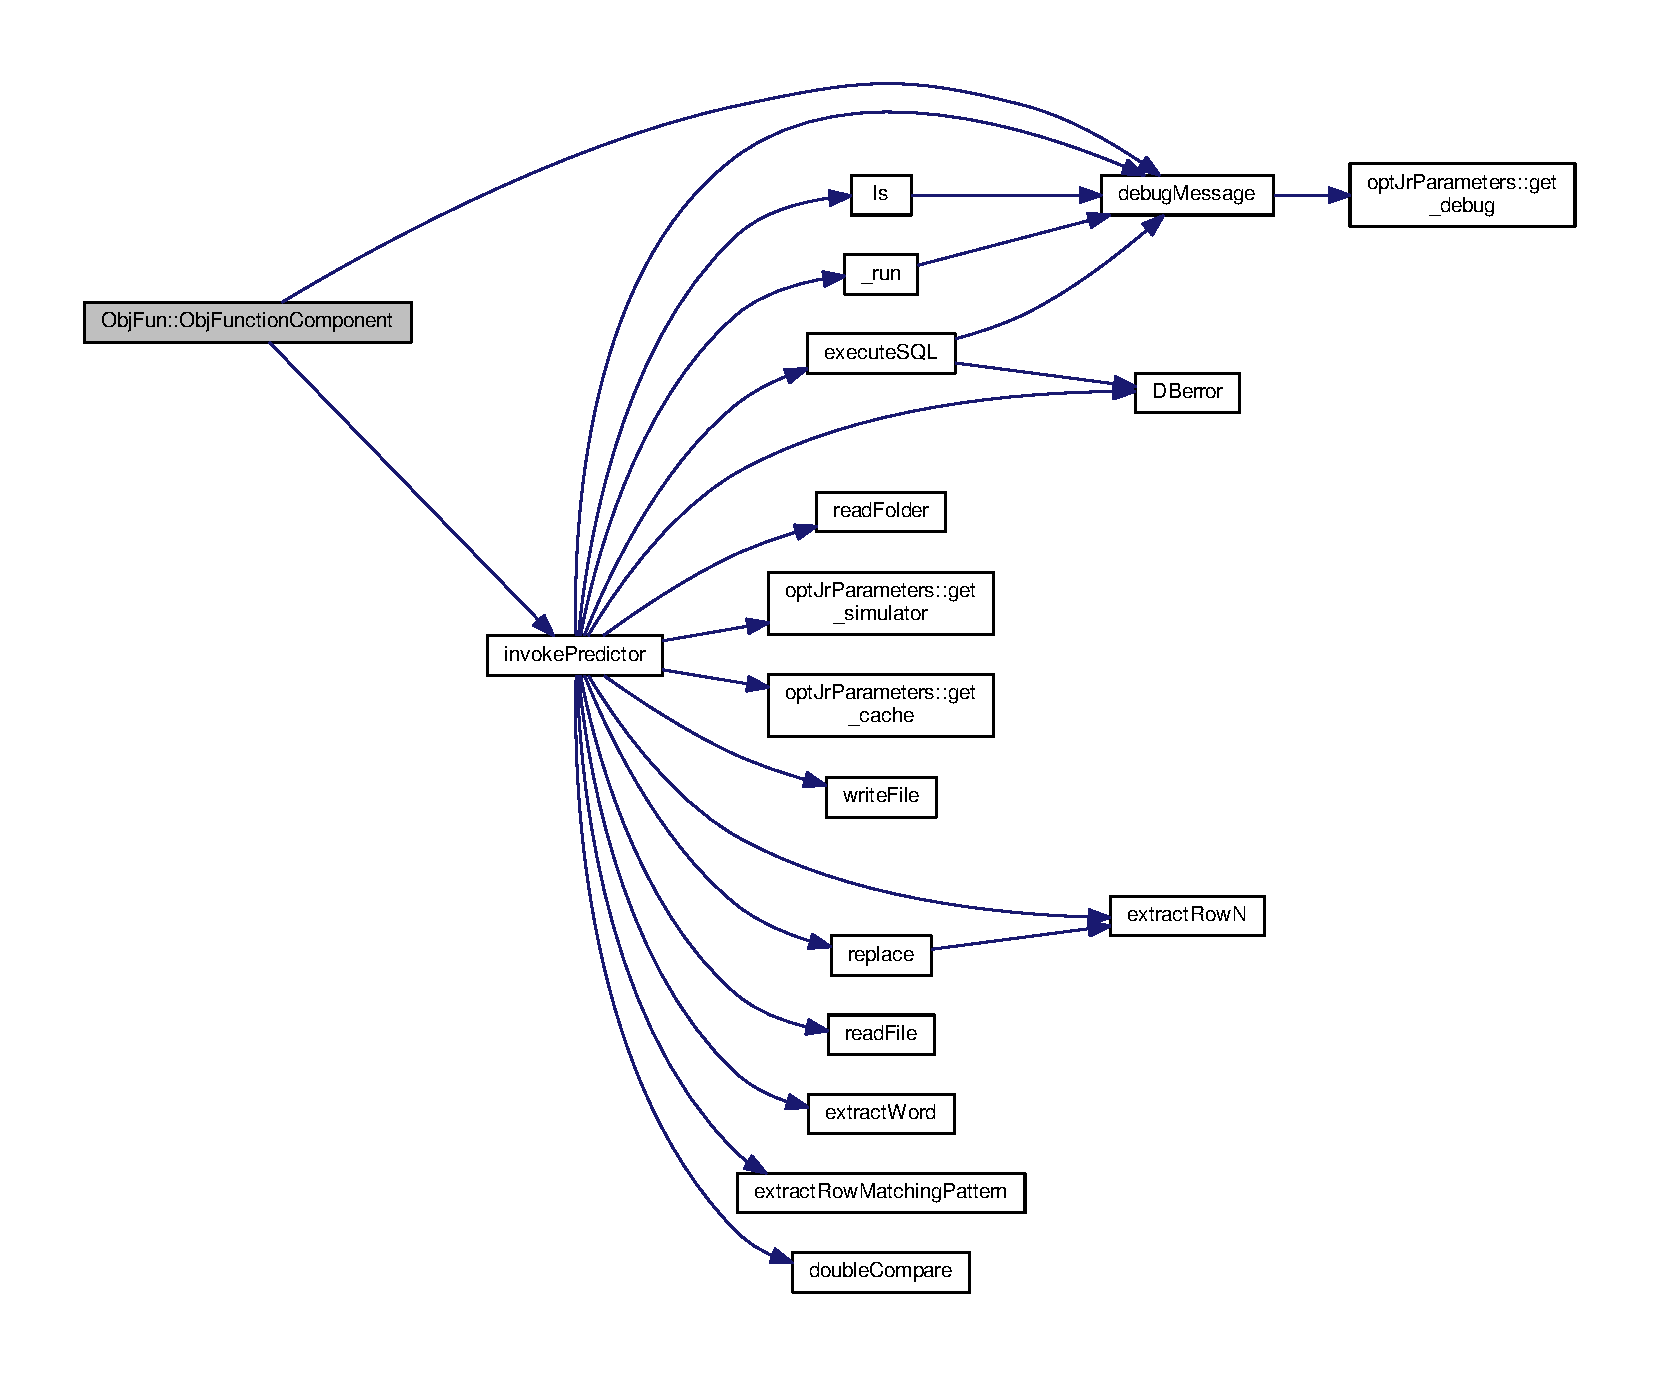
\includegraphics[width=350pt]{classObjFun_a7c9ecaa07ca776eb64f6e73f84513bc7_cgraph}
\end{center}
\end{figure}




Here is the caller graph for this function\-:\nopagebreak
\begin{figure}[H]
\begin{center}
\leavevmode
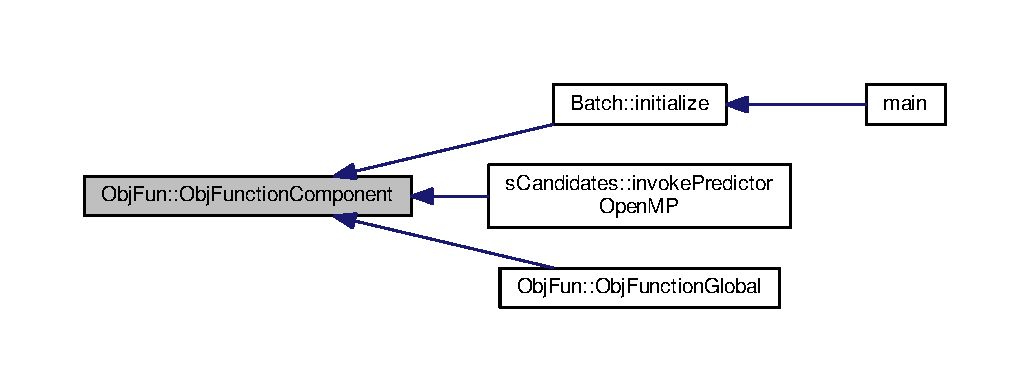
\includegraphics[width=350pt]{classObjFun_a7c9ecaa07ca776eb64f6e73f84513bc7_icgraph}
\end{center}
\end{figure}


\hypertarget{classObjFun_abb89a994d34b44ec4cb6e0e2562c0107}{\index{Obj\-Fun@{Obj\-Fun}!Obj\-Function\-Component\-Approx@{Obj\-Function\-Component\-Approx}}
\index{Obj\-Function\-Component\-Approx@{Obj\-Function\-Component\-Approx}!ObjFun@{Obj\-Fun}}
\subsubsection[{Obj\-Function\-Component\-Approx}]{\setlength{\rightskip}{0pt plus 5cm}double Obj\-Fun\-::\-Obj\-Function\-Component\-Approx (
\begin{DoxyParamCaption}
\item[{{\bf Application} \&}]{App, }
\item[{{\bf opt\-Jr\-Parameters} \&}]{par}
\end{DoxyParamCaption}
)\hspace{0.3cm}{\ttfamily [static]}}}\label{classObjFun_abb89a994d34b44ec4cb6e0e2562c0107}


Here is the call graph for this function\-:\nopagebreak
\begin{figure}[H]
\begin{center}
\leavevmode
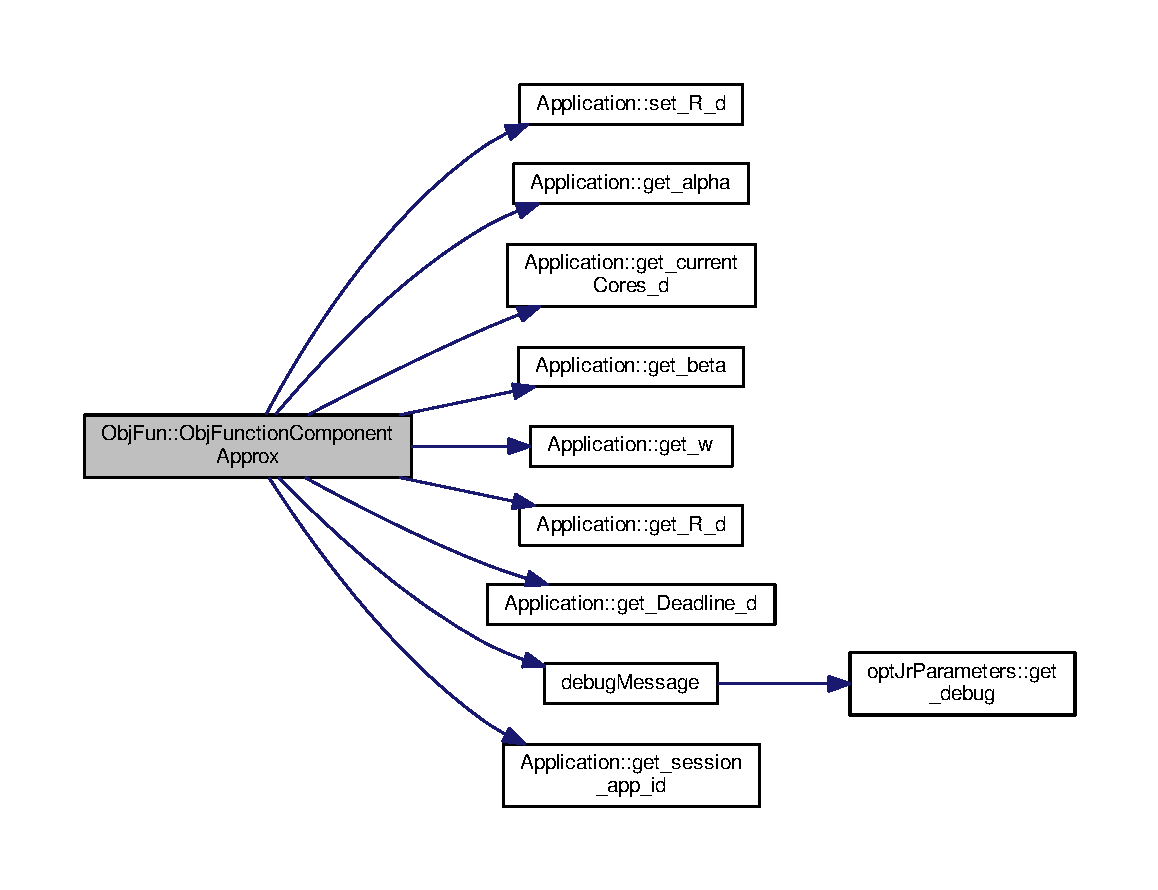
\includegraphics[width=350pt]{classObjFun_abb89a994d34b44ec4cb6e0e2562c0107_cgraph}
\end{center}
\end{figure}




Here is the caller graph for this function\-:\nopagebreak
\begin{figure}[H]
\begin{center}
\leavevmode
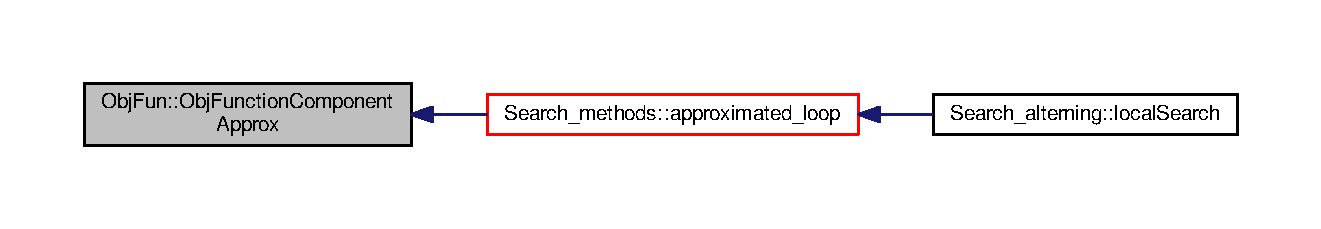
\includegraphics[width=350pt]{classObjFun_abb89a994d34b44ec4cb6e0e2562c0107_icgraph}
\end{center}
\end{figure}


\hypertarget{classObjFun_ab36af3a1d85dbcaa79dc9b582b00928b}{\index{Obj\-Fun@{Obj\-Fun}!Obj\-Function\-Global@{Obj\-Function\-Global}}
\index{Obj\-Function\-Global@{Obj\-Function\-Global}!ObjFun@{Obj\-Fun}}
\subsubsection[{Obj\-Function\-Global}]{\setlength{\rightskip}{0pt plus 5cm}double Obj\-Fun\-::\-Obj\-Function\-Global (
\begin{DoxyParamCaption}
\item[{{\bf s\-Configuration} \&}]{configuration, }
\item[{M\-Y\-S\-Q\-L $\ast$}]{conn, }
\item[{{\bf Batch} \&}]{App\-\_\-manager, }
\item[{{\bf opt\-Jr\-Parameters} \&}]{par}
\end{DoxyParamCaption}
)\hspace{0.3cm}{\ttfamily [static]}}}\label{classObjFun_ab36af3a1d85dbcaa79dc9b582b00928b}


Here is the call graph for this function\-:\nopagebreak
\begin{figure}[H]
\begin{center}
\leavevmode
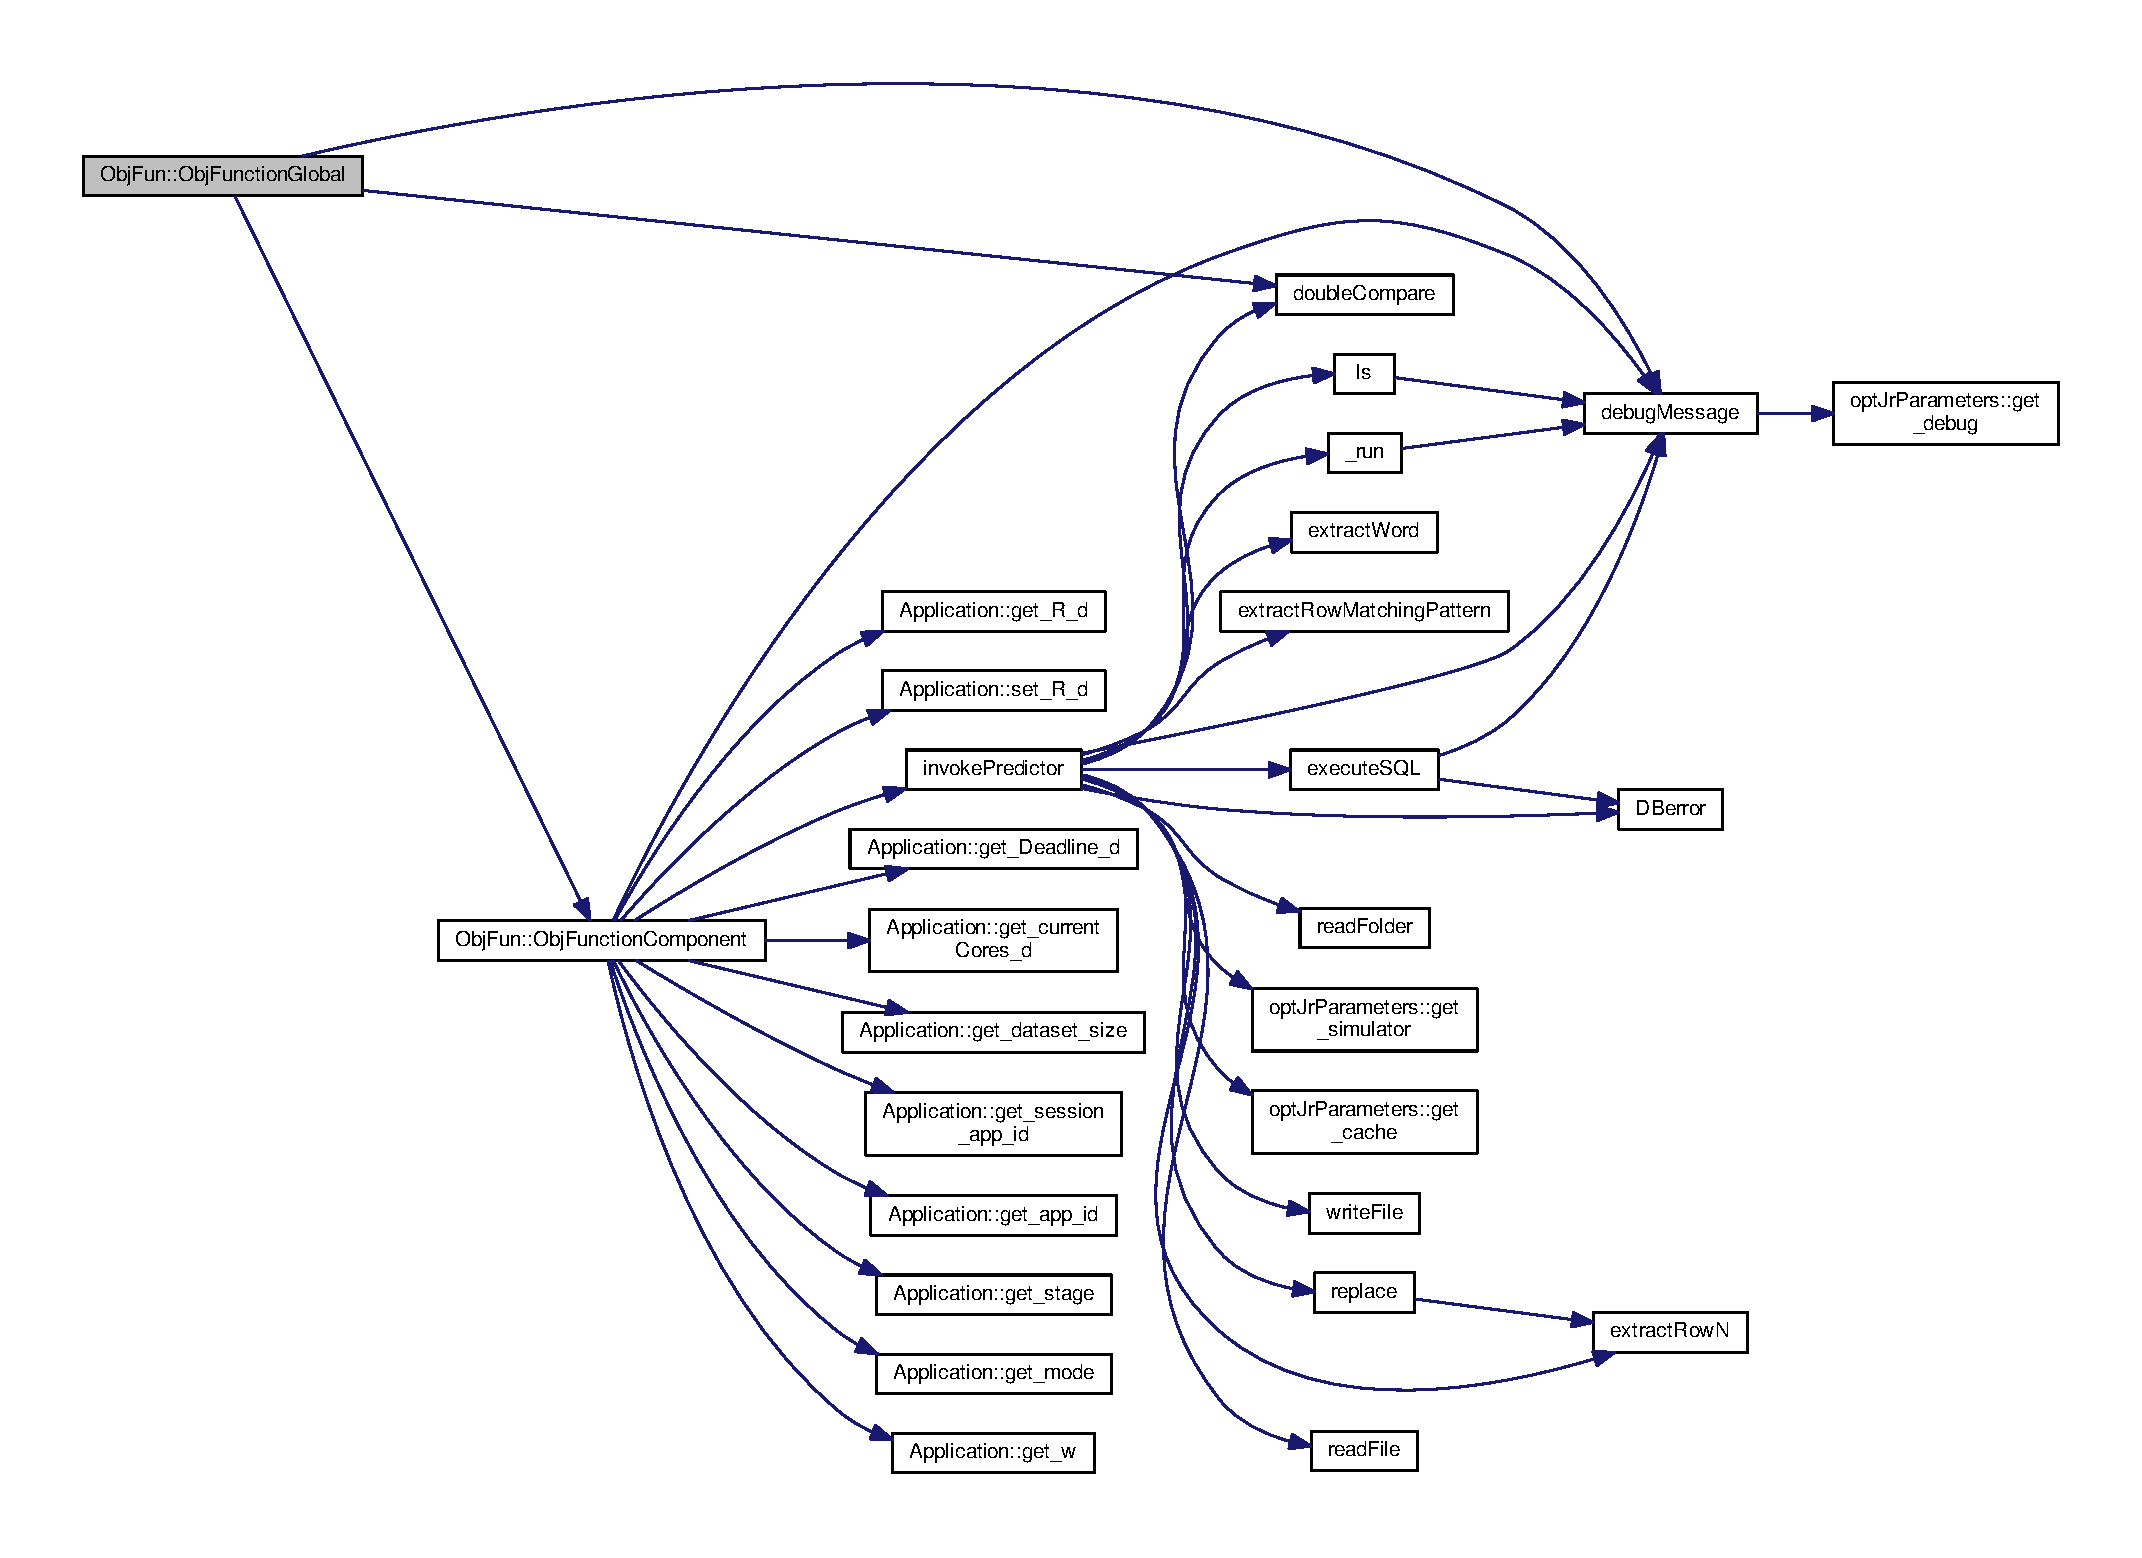
\includegraphics[width=350pt]{classObjFun_ab36af3a1d85dbcaa79dc9b582b00928b_cgraph}
\end{center}
\end{figure}




The documentation for this class was generated from the following files\-:\begin{DoxyCompactItemize}
\item 
/vagrant/\-P\-R\-O\-J\-E\-C\-T\-\_\-\-S\-P\-A\-R\-K/\-P\-A\-C\-S\-\_\-\-P\-R\-O\-J\-E\-C\-T/opt\-\_\-jr/src/\hyperlink{objectiveFunction_8hh}{objective\-Function.\-hh}\item 
/vagrant/\-P\-R\-O\-J\-E\-C\-T\-\_\-\-S\-P\-A\-R\-K/\-P\-A\-C\-S\-\_\-\-P\-R\-O\-J\-E\-C\-T/opt\-\_\-jr/src/\hyperlink{objectiveFunction_8cpp}{objective\-Function.\-cpp}\end{DoxyCompactItemize}

\hypertarget{classoptJrParameters}{\section{opt\-Jr\-Parameters Class Reference}
\label{classoptJrParameters}\index{opt\-Jr\-Parameters@{opt\-Jr\-Parameters}}
}


{\ttfamily \#include $<$optjr\-Parameters.\-hh$>$}

\subsection*{Public Member Functions}
\begin{DoxyCompactItemize}
\item 
\hyperlink{classoptJrParameters_a76f806d48141b4b4c7a215c2645011de}{opt\-Jr\-Parameters} (char $\ast$$\ast$args, int argc)
\item 
const std\-::string \hyperlink{classoptJrParameters_a8dcc738e721b3df88c2622712ed83414}{get\-\_\-filename} ()
\item 
const int \hyperlink{classoptJrParameters_a64016f274261a7a7d74d8460bb7e2ee4}{get\-\_\-debug} ()
\item 
const int \hyperlink{classoptJrParameters_ac698812fa1177c71eb46dc61d2e5af77}{get\-\_\-cache} ()
\item 
const int \hyperlink{classoptJrParameters_a7eec5151603fd03276b6fcf6213f9f90}{get\-\_\-global\-F\-Ocalculation} ()
\item 
const int \hyperlink{classoptJrParameters_a8274b4a95698ce1681147fdddbced0d8}{get\-\_\-\-K} ()
\item 
const int \hyperlink{classoptJrParameters_a199e3fc83f3efb82fc63796a540d6589}{get\-\_\-simulator} ()
\item 
const int \hyperlink{classoptJrParameters_a9bb0e783bd6bf555e86cea874f13cb4f}{get\-\_\-number} ()
\item 
const int \hyperlink{classoptJrParameters_a73340961e894748c6c143284e0b278fa}{get\-\_\-max\-Iteration} ()
\end{DoxyCompactItemize}


\subsection{Constructor \& Destructor Documentation}
\hypertarget{classoptJrParameters_a76f806d48141b4b4c7a215c2645011de}{\index{opt\-Jr\-Parameters@{opt\-Jr\-Parameters}!opt\-Jr\-Parameters@{opt\-Jr\-Parameters}}
\index{opt\-Jr\-Parameters@{opt\-Jr\-Parameters}!optJrParameters@{opt\-Jr\-Parameters}}
\subsubsection[{opt\-Jr\-Parameters}]{\setlength{\rightskip}{0pt plus 5cm}opt\-Jr\-Parameters\-::opt\-Jr\-Parameters (
\begin{DoxyParamCaption}
\item[{char $\ast$$\ast$}]{args, }
\item[{int}]{argc}
\end{DoxyParamCaption}
)}}\label{classoptJrParameters_a76f806d48141b4b4c7a215c2645011de}


Here is the call graph for this function\-:\nopagebreak
\begin{figure}[H]
\begin{center}
\leavevmode
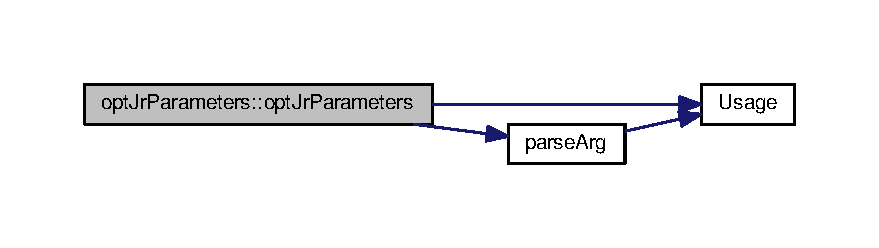
\includegraphics[width=350pt]{classoptJrParameters_a76f806d48141b4b4c7a215c2645011de_cgraph}
\end{center}
\end{figure}




\subsection{Member Function Documentation}
\hypertarget{classoptJrParameters_ac698812fa1177c71eb46dc61d2e5af77}{\index{opt\-Jr\-Parameters@{opt\-Jr\-Parameters}!get\-\_\-cache@{get\-\_\-cache}}
\index{get\-\_\-cache@{get\-\_\-cache}!optJrParameters@{opt\-Jr\-Parameters}}
\subsubsection[{get\-\_\-cache}]{\setlength{\rightskip}{0pt plus 5cm}const int opt\-Jr\-Parameters\-::get\-\_\-cache (
\begin{DoxyParamCaption}
{}
\end{DoxyParamCaption}
)}}\label{classoptJrParameters_ac698812fa1177c71eb46dc61d2e5af77}


Here is the caller graph for this function\-:\nopagebreak
\begin{figure}[H]
\begin{center}
\leavevmode
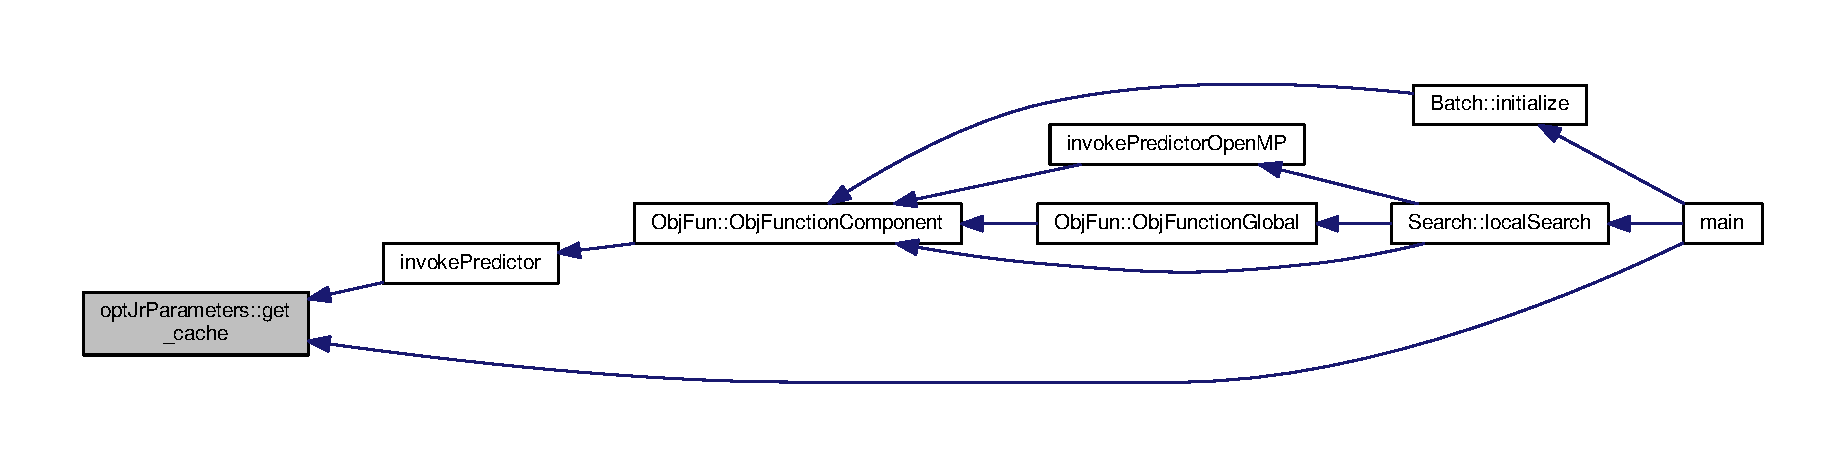
\includegraphics[width=262pt]{classoptJrParameters_ac698812fa1177c71eb46dc61d2e5af77_icgraph}
\end{center}
\end{figure}


\hypertarget{classoptJrParameters_a64016f274261a7a7d74d8460bb7e2ee4}{\index{opt\-Jr\-Parameters@{opt\-Jr\-Parameters}!get\-\_\-debug@{get\-\_\-debug}}
\index{get\-\_\-debug@{get\-\_\-debug}!optJrParameters@{opt\-Jr\-Parameters}}
\subsubsection[{get\-\_\-debug}]{\setlength{\rightskip}{0pt plus 5cm}const int opt\-Jr\-Parameters\-::get\-\_\-debug (
\begin{DoxyParamCaption}
{}
\end{DoxyParamCaption}
)}}\label{classoptJrParameters_a64016f274261a7a7d74d8460bb7e2ee4}


Here is the caller graph for this function\-:\nopagebreak
\begin{figure}[H]
\begin{center}
\leavevmode
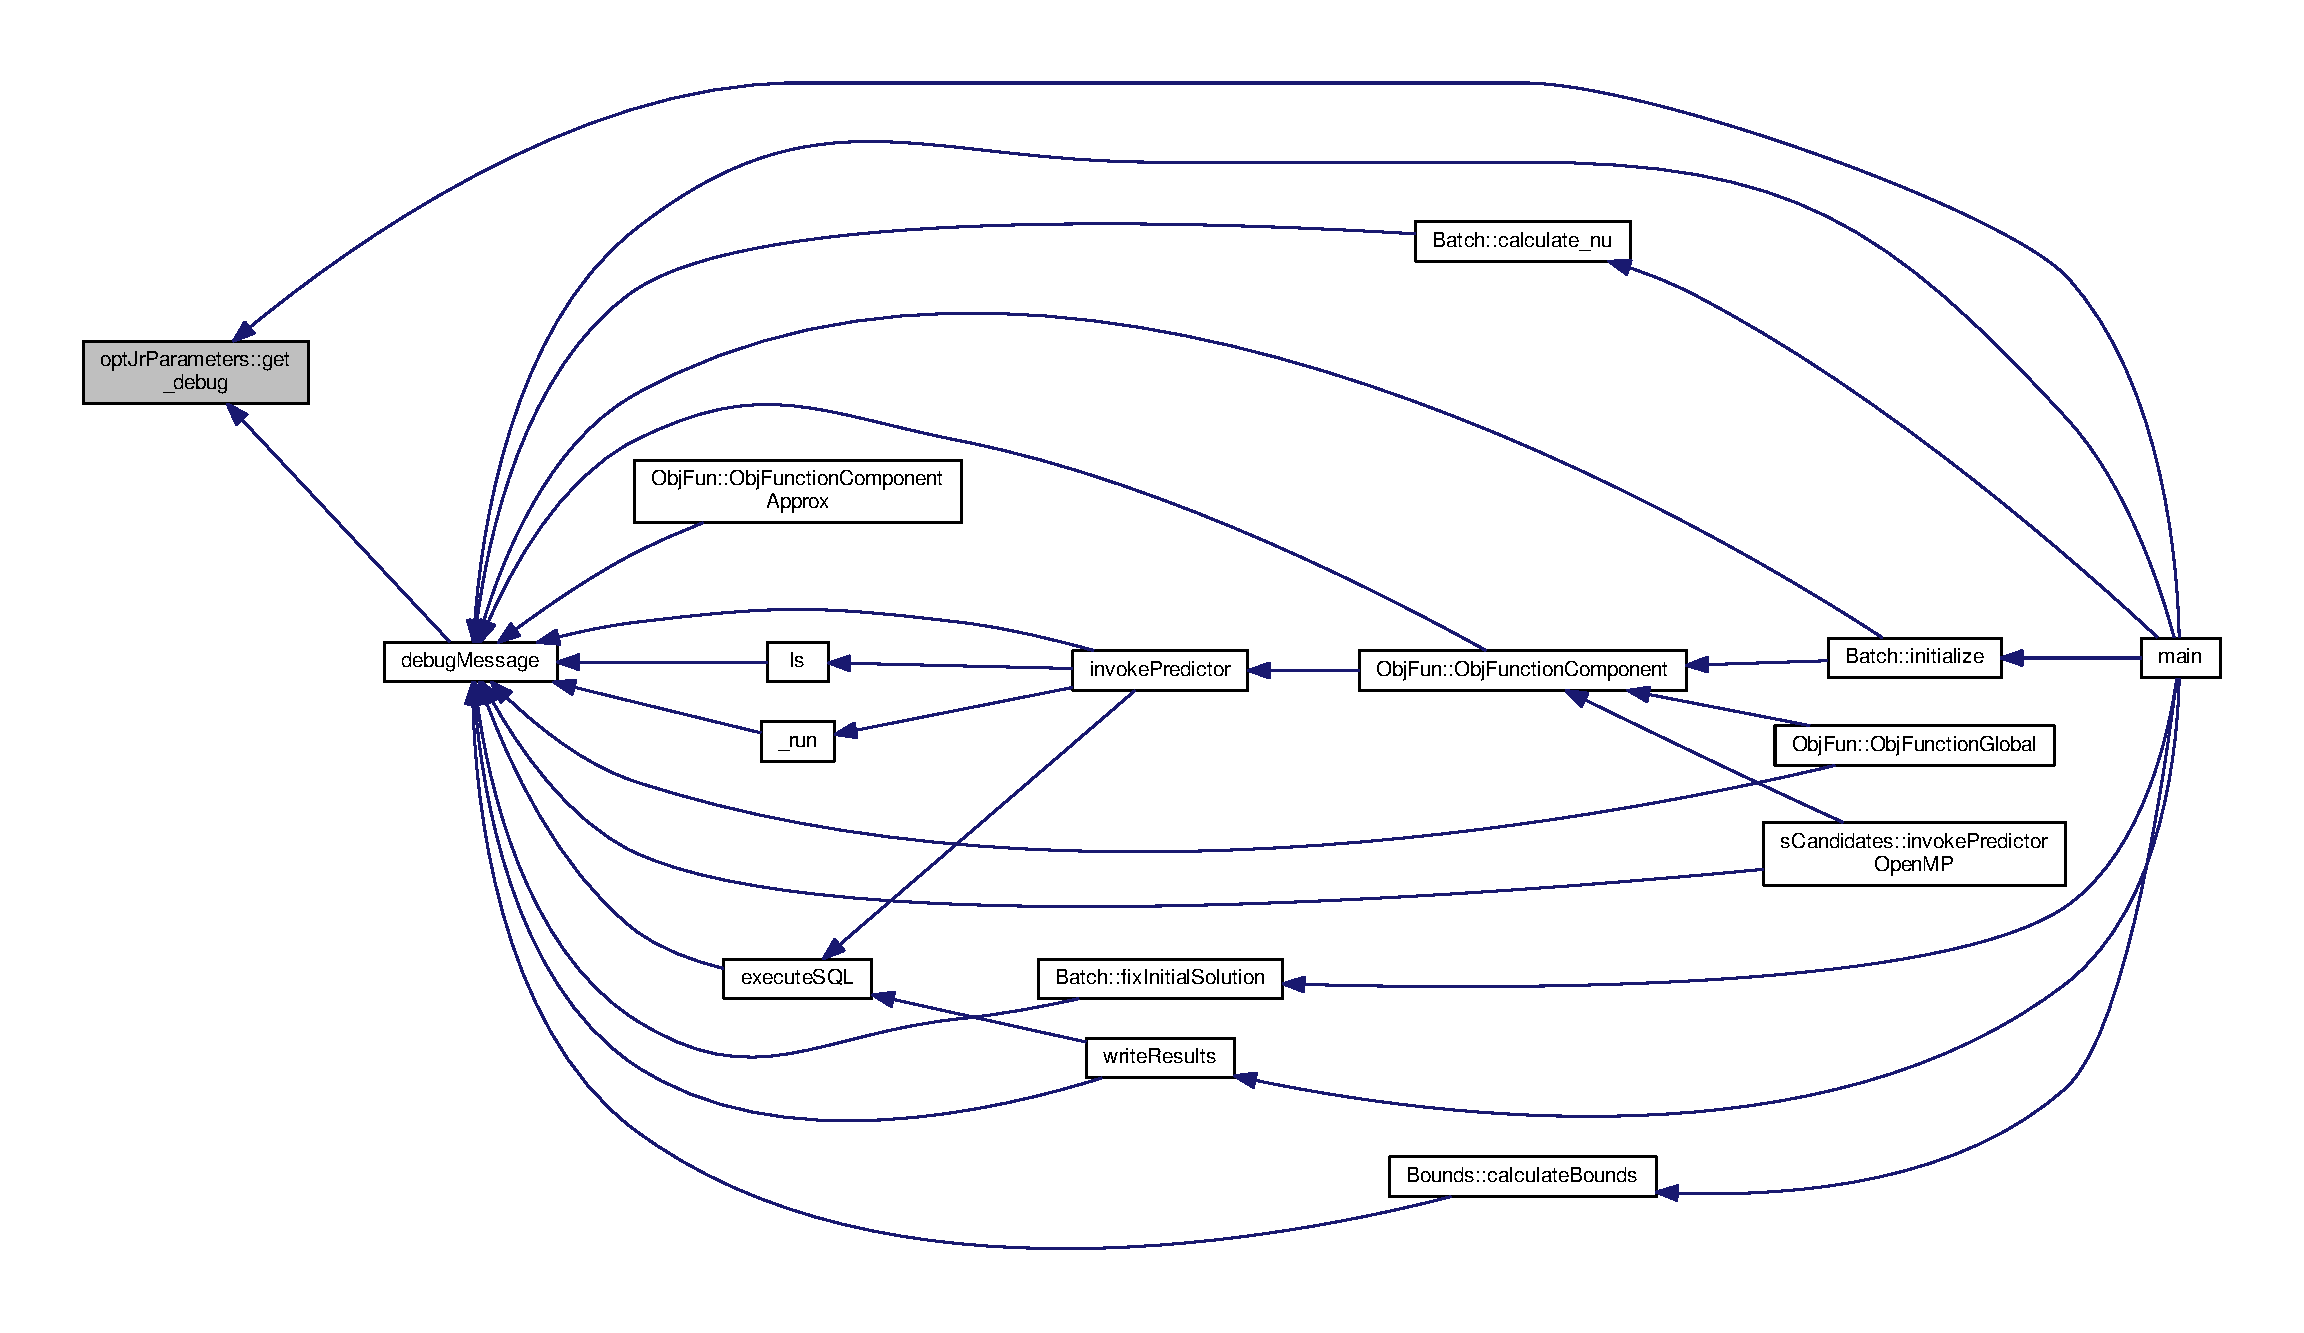
\includegraphics[width=350pt]{classoptJrParameters_a64016f274261a7a7d74d8460bb7e2ee4_icgraph}
\end{center}
\end{figure}


\hypertarget{classoptJrParameters_a8dcc738e721b3df88c2622712ed83414}{\index{opt\-Jr\-Parameters@{opt\-Jr\-Parameters}!get\-\_\-filename@{get\-\_\-filename}}
\index{get\-\_\-filename@{get\-\_\-filename}!optJrParameters@{opt\-Jr\-Parameters}}
\subsubsection[{get\-\_\-filename}]{\setlength{\rightskip}{0pt plus 5cm}const std\-::string opt\-Jr\-Parameters\-::get\-\_\-filename (
\begin{DoxyParamCaption}
{}
\end{DoxyParamCaption}
)}}\label{classoptJrParameters_a8dcc738e721b3df88c2622712ed83414}


Here is the caller graph for this function\-:\nopagebreak
\begin{figure}[H]
\begin{center}
\leavevmode
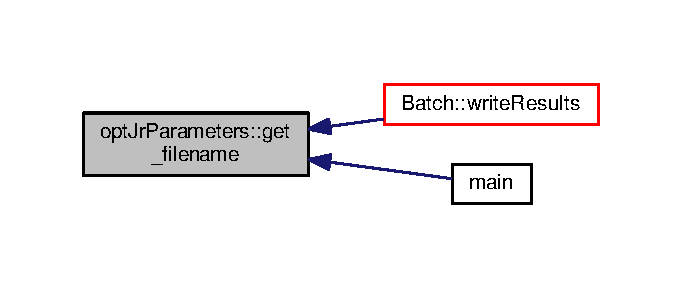
\includegraphics[width=262pt]{classoptJrParameters_a8dcc738e721b3df88c2622712ed83414_icgraph}
\end{center}
\end{figure}


\hypertarget{classoptJrParameters_a7eec5151603fd03276b6fcf6213f9f90}{\index{opt\-Jr\-Parameters@{opt\-Jr\-Parameters}!get\-\_\-global\-F\-Ocalculation@{get\-\_\-global\-F\-Ocalculation}}
\index{get\-\_\-global\-F\-Ocalculation@{get\-\_\-global\-F\-Ocalculation}!optJrParameters@{opt\-Jr\-Parameters}}
\subsubsection[{get\-\_\-global\-F\-Ocalculation}]{\setlength{\rightskip}{0pt plus 5cm}const int opt\-Jr\-Parameters\-::get\-\_\-global\-F\-Ocalculation (
\begin{DoxyParamCaption}
{}
\end{DoxyParamCaption}
)}}\label{classoptJrParameters_a7eec5151603fd03276b6fcf6213f9f90}


Here is the caller graph for this function\-:\nopagebreak
\begin{figure}[H]
\begin{center}
\leavevmode
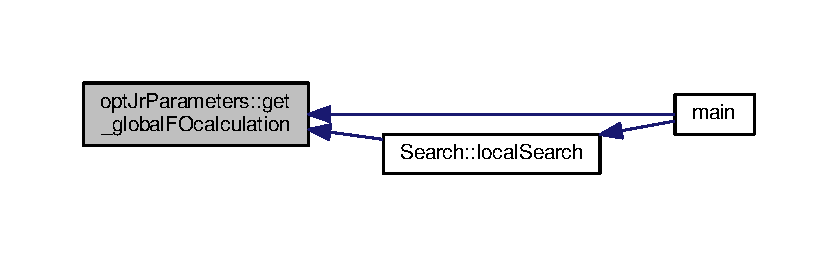
\includegraphics[width=262pt]{classoptJrParameters_a7eec5151603fd03276b6fcf6213f9f90_icgraph}
\end{center}
\end{figure}


\hypertarget{classoptJrParameters_a8274b4a95698ce1681147fdddbced0d8}{\index{opt\-Jr\-Parameters@{opt\-Jr\-Parameters}!get\-\_\-\-K@{get\-\_\-\-K}}
\index{get\-\_\-\-K@{get\-\_\-\-K}!optJrParameters@{opt\-Jr\-Parameters}}
\subsubsection[{get\-\_\-\-K}]{\setlength{\rightskip}{0pt plus 5cm}const int opt\-Jr\-Parameters\-::get\-\_\-\-K (
\begin{DoxyParamCaption}
{}
\end{DoxyParamCaption}
)}}\label{classoptJrParameters_a8274b4a95698ce1681147fdddbced0d8}


Here is the caller graph for this function\-:\nopagebreak
\begin{figure}[H]
\begin{center}
\leavevmode
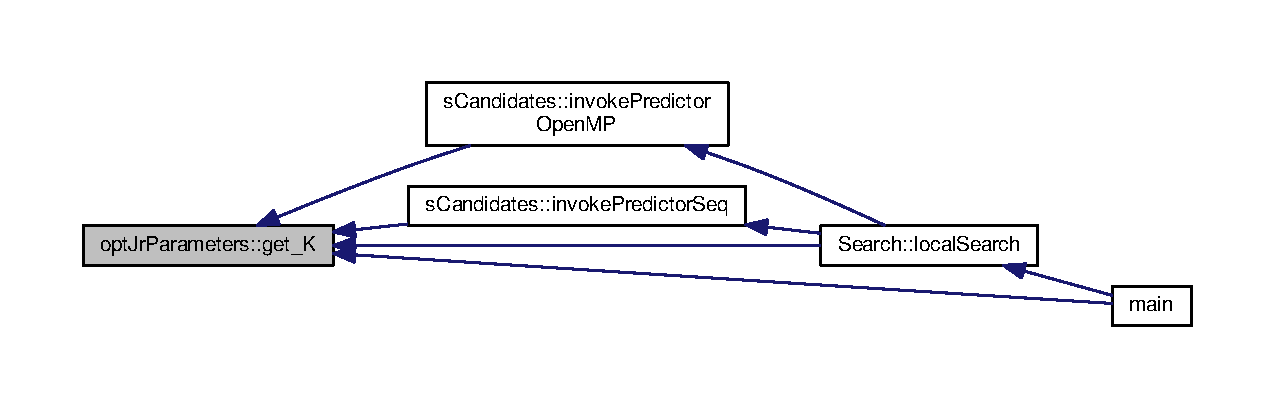
\includegraphics[width=350pt]{classoptJrParameters_a8274b4a95698ce1681147fdddbced0d8_icgraph}
\end{center}
\end{figure}


\hypertarget{classoptJrParameters_a73340961e894748c6c143284e0b278fa}{\index{opt\-Jr\-Parameters@{opt\-Jr\-Parameters}!get\-\_\-max\-Iteration@{get\-\_\-max\-Iteration}}
\index{get\-\_\-max\-Iteration@{get\-\_\-max\-Iteration}!optJrParameters@{opt\-Jr\-Parameters}}
\subsubsection[{get\-\_\-max\-Iteration}]{\setlength{\rightskip}{0pt plus 5cm}const int opt\-Jr\-Parameters\-::get\-\_\-max\-Iteration (
\begin{DoxyParamCaption}
{}
\end{DoxyParamCaption}
)}}\label{classoptJrParameters_a73340961e894748c6c143284e0b278fa}


Here is the caller graph for this function\-:\nopagebreak
\begin{figure}[H]
\begin{center}
\leavevmode
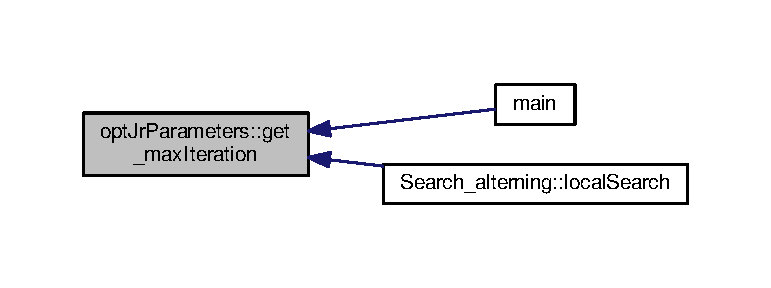
\includegraphics[width=350pt]{classoptJrParameters_a73340961e894748c6c143284e0b278fa_icgraph}
\end{center}
\end{figure}


\hypertarget{classoptJrParameters_a9bb0e783bd6bf555e86cea874f13cb4f}{\index{opt\-Jr\-Parameters@{opt\-Jr\-Parameters}!get\-\_\-number@{get\-\_\-number}}
\index{get\-\_\-number@{get\-\_\-number}!optJrParameters@{opt\-Jr\-Parameters}}
\subsubsection[{get\-\_\-number}]{\setlength{\rightskip}{0pt plus 5cm}const int opt\-Jr\-Parameters\-::get\-\_\-number (
\begin{DoxyParamCaption}
{}
\end{DoxyParamCaption}
)}}\label{classoptJrParameters_a9bb0e783bd6bf555e86cea874f13cb4f}


Here is the caller graph for this function\-:\nopagebreak
\begin{figure}[H]
\begin{center}
\leavevmode
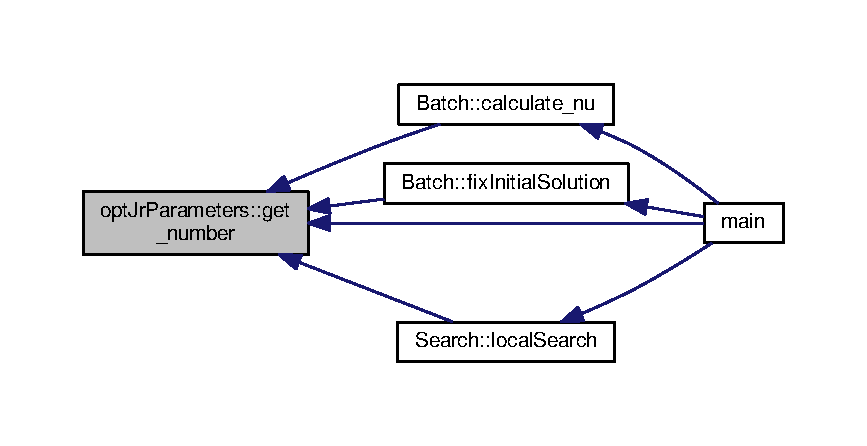
\includegraphics[width=350pt]{classoptJrParameters_a9bb0e783bd6bf555e86cea874f13cb4f_icgraph}
\end{center}
\end{figure}


\hypertarget{classoptJrParameters_a199e3fc83f3efb82fc63796a540d6589}{\index{opt\-Jr\-Parameters@{opt\-Jr\-Parameters}!get\-\_\-simulator@{get\-\_\-simulator}}
\index{get\-\_\-simulator@{get\-\_\-simulator}!optJrParameters@{opt\-Jr\-Parameters}}
\subsubsection[{get\-\_\-simulator}]{\setlength{\rightskip}{0pt plus 5cm}const int opt\-Jr\-Parameters\-::get\-\_\-simulator (
\begin{DoxyParamCaption}
{}
\end{DoxyParamCaption}
)}}\label{classoptJrParameters_a199e3fc83f3efb82fc63796a540d6589}


Here is the caller graph for this function\-:\nopagebreak
\begin{figure}[H]
\begin{center}
\leavevmode
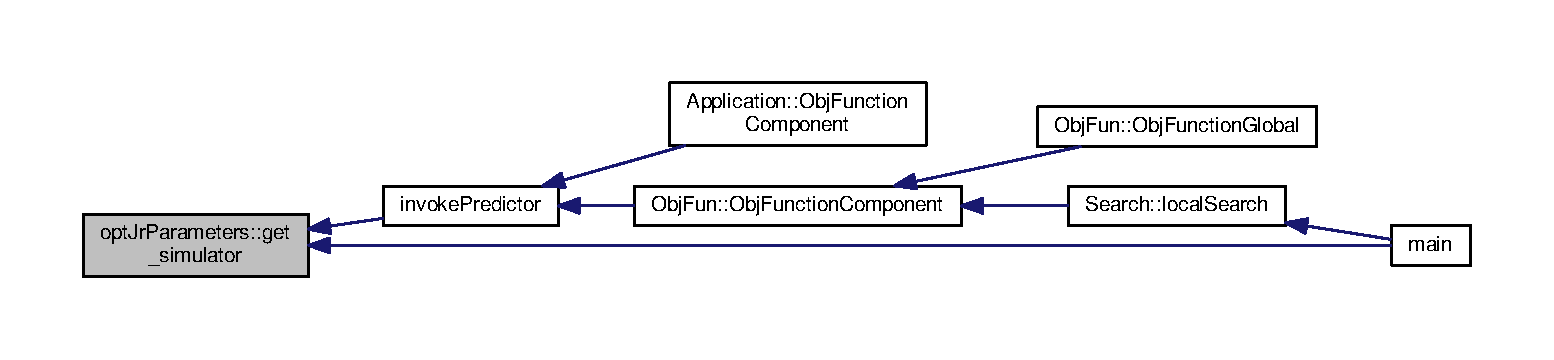
\includegraphics[width=350pt]{classoptJrParameters_a199e3fc83f3efb82fc63796a540d6589_icgraph}
\end{center}
\end{figure}




The documentation for this class was generated from the following files\-:\begin{DoxyCompactItemize}
\item 
/vagrant/\-P\-R\-O\-J\-E\-C\-T\-\_\-\-S\-P\-A\-R\-K/\-P\-A\-C\-S\-\_\-\-P\-R\-O\-J\-E\-C\-T/opt\-\_\-jr/src/\hyperlink{optjrParameters_8hh}{optjr\-Parameters.\-hh}\item 
/vagrant/\-P\-R\-O\-J\-E\-C\-T\-\_\-\-S\-P\-A\-R\-K/\-P\-A\-C\-S\-\_\-\-P\-R\-O\-J\-E\-C\-T/opt\-\_\-jr/src/\hyperlink{optjrparameters_8cpp}{optjrparameters.\-cpp}\end{DoxyCompactItemize}

\hypertarget{classsAlphaBetaManagement}{\section{s\-Alpha\-Beta\-Management Class Reference}
\label{classsAlphaBetaManagement}\index{s\-Alpha\-Beta\-Management@{s\-Alpha\-Beta\-Management}}
}


{\ttfamily \#include $<$application.\-hh$>$}



Collaboration diagram for s\-Alpha\-Beta\-Management\-:\nopagebreak
\begin{figure}[H]
\begin{center}
\leavevmode
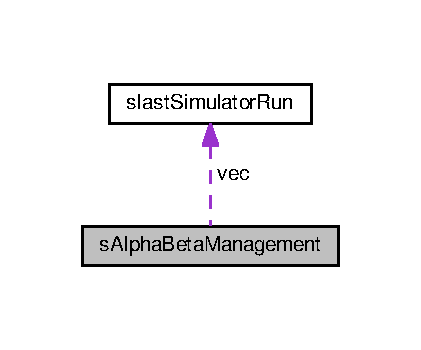
\includegraphics[width=202pt]{classsAlphaBetaManagement__coll__graph}
\end{center}
\end{figure}
\subsection*{Public Attributes}
\begin{DoxyCompactItemize}
\item 
\hyperlink{classslastSimulatorRun}{slast\-Simulator\-Run} \hyperlink{classsAlphaBetaManagement_af9fd5945bd8e0566f69804372b5ca01d}{vec} \mbox{[}\hyperlink{application_8hh_a0f42c303bf81baaf28a6fa46e2b3e58e}{H\-Y\-P\-\_\-\-I\-N\-T\-E\-R\-P\-O\-L\-A\-T\-I\-O\-N\-\_\-\-P\-O\-I\-N\-T\-S}\mbox{]}
\item 
int \hyperlink{classsAlphaBetaManagement_acfd2318c63ee03cd1e25904deedfe88f}{index}
\end{DoxyCompactItemize}


\subsection{Member Data Documentation}
\hypertarget{classsAlphaBetaManagement_acfd2318c63ee03cd1e25904deedfe88f}{\index{s\-Alpha\-Beta\-Management@{s\-Alpha\-Beta\-Management}!index@{index}}
\index{index@{index}!sAlphaBetaManagement@{s\-Alpha\-Beta\-Management}}
\subsubsection[{index}]{\setlength{\rightskip}{0pt plus 5cm}int s\-Alpha\-Beta\-Management\-::index}}\label{classsAlphaBetaManagement_acfd2318c63ee03cd1e25904deedfe88f}
\hypertarget{classsAlphaBetaManagement_af9fd5945bd8e0566f69804372b5ca01d}{\index{s\-Alpha\-Beta\-Management@{s\-Alpha\-Beta\-Management}!vec@{vec}}
\index{vec@{vec}!sAlphaBetaManagement@{s\-Alpha\-Beta\-Management}}
\subsubsection[{vec}]{\setlength{\rightskip}{0pt plus 5cm}{\bf slast\-Simulator\-Run} s\-Alpha\-Beta\-Management\-::vec\mbox{[}{\bf H\-Y\-P\-\_\-\-I\-N\-T\-E\-R\-P\-O\-L\-A\-T\-I\-O\-N\-\_\-\-P\-O\-I\-N\-T\-S}\mbox{]}}}\label{classsAlphaBetaManagement_af9fd5945bd8e0566f69804372b5ca01d}


The documentation for this class was generated from the following file\-:\begin{DoxyCompactItemize}
\item 
/vagrant/\-P\-R\-O\-J\-E\-C\-T\-\_\-\-S\-P\-A\-R\-K/\-P\-A\-C\-S\-\_\-\-P\-R\-O\-J\-E\-C\-T/opt\-\_\-jr/src/\hyperlink{application_8hh}{application.\-hh}\end{DoxyCompactItemize}

\hypertarget{classSearch}{\section{Search$<$ Policy $>$ Class Template Reference}
\label{classSearch}\index{Search$<$ Policy $>$@{Search$<$ Policy $>$}}
}


{\ttfamily \#include $<$search.\-hh$>$}



Inheritance diagram for Search$<$ Policy $>$\-:
\nopagebreak
\begin{figure}[H]
\begin{center}
\leavevmode
\includegraphics[width=188pt]{classSearch__inherit__graph}
\end{center}
\end{figure}


Collaboration diagram for Search$<$ Policy $>$\-:
\nopagebreak
\begin{figure}[H]
\begin{center}
\leavevmode
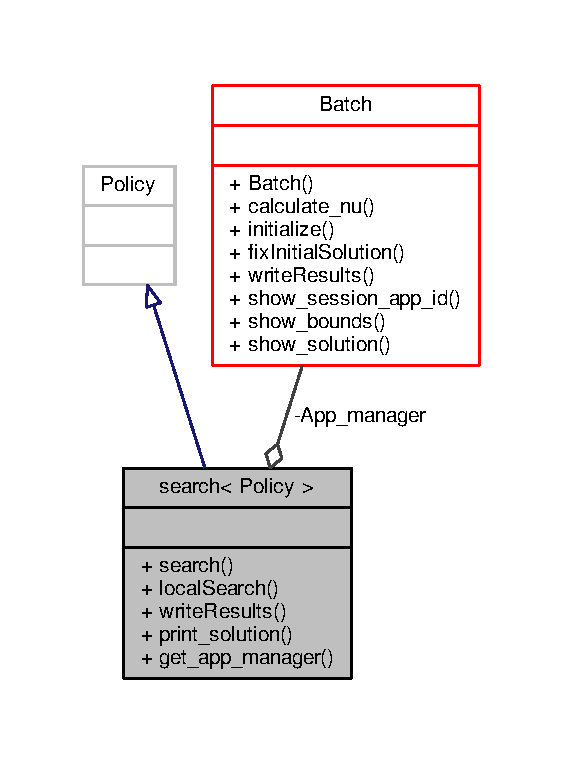
\includegraphics[width=213pt]{classSearch__coll__graph}
\end{center}
\end{figure}
\subsection*{Public Member Functions}
\begin{DoxyCompactItemize}
\item 
\hyperlink{classSearch_a59b826749138fdaa93c41b1e0697da58}{Search} (\hyperlink{classBatch}{Batch} app\-\_\-m)
\item 
void \hyperlink{classSearch_a32d434fae76c18149f8b15aedadc5f75}{local\-\_\-search} (\hyperlink{classConfiguration}{Configuration} \&configuration, M\-Y\-S\-Q\-L $\ast$conn, \hyperlink{classOpt__jr__parameters}{Opt\-\_\-jr\-\_\-parameters} \&par)
\end{DoxyCompactItemize}
\subsection*{Additional Inherited Members}


\subsection{Detailed Description}
\subsubsection*{template$<$class Policy$>$class Search$<$ Policy $>$}

T\-O\-D\-O\-: modify descript. \char`\"{}\-Search\char`\"{} class provides methods to find a solution minimizing the objective function. Actually only one method is supported. 

\subsection{Constructor \& Destructor Documentation}
\hypertarget{classSearch_a59b826749138fdaa93c41b1e0697da58}{\index{Search@{Search}!Search@{Search}}
\index{Search@{Search}!Search@{Search}}
\subsubsection[{Search}]{\setlength{\rightskip}{0pt plus 5cm}template$<$class Policy $>$ {\bf Search}$<$ Policy $>$\-::{\bf Search} (
\begin{DoxyParamCaption}
\item[{{\bf Batch}}]{app\-\_\-m}
\end{DoxyParamCaption}
)\hspace{0.3cm}{\ttfamily [inline]}}}\label{classSearch_a59b826749138fdaa93c41b1e0697da58}


\subsection{Member Function Documentation}
\hypertarget{classSearch_a32d434fae76c18149f8b15aedadc5f75}{\index{Search@{Search}!local\-\_\-search@{local\-\_\-search}}
\index{local\-\_\-search@{local\-\_\-search}!Search@{Search}}
\subsubsection[{local\-\_\-search}]{\setlength{\rightskip}{0pt plus 5cm}template$<$class Policy $>$ void {\bf Search}$<$ Policy $>$\-::local\-\_\-search (
\begin{DoxyParamCaption}
\item[{{\bf Configuration} \&}]{configuration, }
\item[{M\-Y\-S\-Q\-L $\ast$}]{conn, }
\item[{{\bf Opt\-\_\-jr\-\_\-parameters} \&}]{par}
\end{DoxyParamCaption}
)\hspace{0.3cm}{\ttfamily [inline]}, {\ttfamily [virtual]}}}\label{classSearch_a32d434fae76c18149f8b15aedadc5f75}
local\-\_\-search perform a local search of a solution minimizing the objective function; it performs cores exchanges between pairs of application and chooses the best pair. The search stops when no improvements are possible or the maximum number of iteration is reached. The function looks before at approximated values of objective function and then for the potential best pairs it invokes the predictor. 

Implements \hyperlink{classSearch__base_ab3730b1118efbe97065f1ea9715a90dc}{Search\-\_\-base}.



The documentation for this class was generated from the following file\-:\begin{DoxyCompactItemize}
\item 
/vagrant/\-P\-R\-O\-J\-E\-C\-T\-\_\-\-S\-P\-A\-R\-K/\-P\-A\-C\-S\-\_\-\-P\-R\-O\-J\-E\-C\-T/opt\-\_\-jr/src/\hyperlink{search_8hh}{search.\-hh}\end{DoxyCompactItemize}

\hypertarget{classslastSimulatorRun}{\section{slast\-Simulator\-Run Class Reference}
\label{classslastSimulatorRun}\index{slast\-Simulator\-Run@{slast\-Simulator\-Run}}
}


{\ttfamily \#include $<$application.\-hh$>$}

\subsection*{Public Attributes}
\begin{DoxyCompactItemize}
\item 
int \hyperlink{classslastSimulatorRun_a709891b6cab0506a591c1979f1001561}{n\-Cores}
\item 
double \hyperlink{classslastSimulatorRun_a0f5480e725b0d25893d8b983d5971d5e}{R}
\end{DoxyCompactItemize}


\subsection{Member Data Documentation}
\hypertarget{classslastSimulatorRun_a709891b6cab0506a591c1979f1001561}{\index{slast\-Simulator\-Run@{slast\-Simulator\-Run}!n\-Cores@{n\-Cores}}
\index{n\-Cores@{n\-Cores}!slastSimulatorRun@{slast\-Simulator\-Run}}
\subsubsection[{n\-Cores}]{\setlength{\rightskip}{0pt plus 5cm}int slast\-Simulator\-Run\-::n\-Cores}}\label{classslastSimulatorRun_a709891b6cab0506a591c1979f1001561}
\hypertarget{classslastSimulatorRun_a0f5480e725b0d25893d8b983d5971d5e}{\index{slast\-Simulator\-Run@{slast\-Simulator\-Run}!R@{R}}
\index{R@{R}!slastSimulatorRun@{slast\-Simulator\-Run}}
\subsubsection[{R}]{\setlength{\rightskip}{0pt plus 5cm}double slast\-Simulator\-Run\-::\-R}}\label{classslastSimulatorRun_a0f5480e725b0d25893d8b983d5971d5e}


The documentation for this class was generated from the following file\-:\begin{DoxyCompactItemize}
\item 
/vagrant/\-P\-R\-O\-J\-E\-C\-T\-\_\-\-S\-P\-A\-R\-K/\-P\-A\-C\-S\-\_\-\-P\-R\-O\-J\-E\-C\-T/opt\-\_\-jr/src/\hyperlink{application_8hh}{application.\-hh}\end{DoxyCompactItemize}

\chapter{File Documentation}
\hypertarget{appByWeight_8cpp}{\section{/vagrant/\-P\-R\-O\-J\-E\-C\-T\-\_\-\-S\-P\-A\-R\-K/\-P\-A\-C\-S\-\_\-\-P\-R\-O\-J\-E\-C\-T/opt\-\_\-jr/src/app\-By\-Weight.cpp File Reference}
\label{appByWeight_8cpp}\index{/vagrant/\-P\-R\-O\-J\-E\-C\-T\-\_\-\-S\-P\-A\-R\-K/\-P\-A\-C\-S\-\_\-\-P\-R\-O\-J\-E\-C\-T/opt\-\_\-jr/src/app\-By\-Weight.\-cpp@{/vagrant/\-P\-R\-O\-J\-E\-C\-T\-\_\-\-S\-P\-A\-R\-K/\-P\-A\-C\-S\-\_\-\-P\-R\-O\-J\-E\-C\-T/opt\-\_\-jr/src/app\-By\-Weight.\-cpp}}
}
{\ttfamily \#include \char`\"{}app\-By\-Weight.\-hh\char`\"{}}\\*
Include dependency graph for app\-By\-Weight.\-cpp\-:
\nopagebreak
\begin{figure}[H]
\begin{center}
\leavevmode
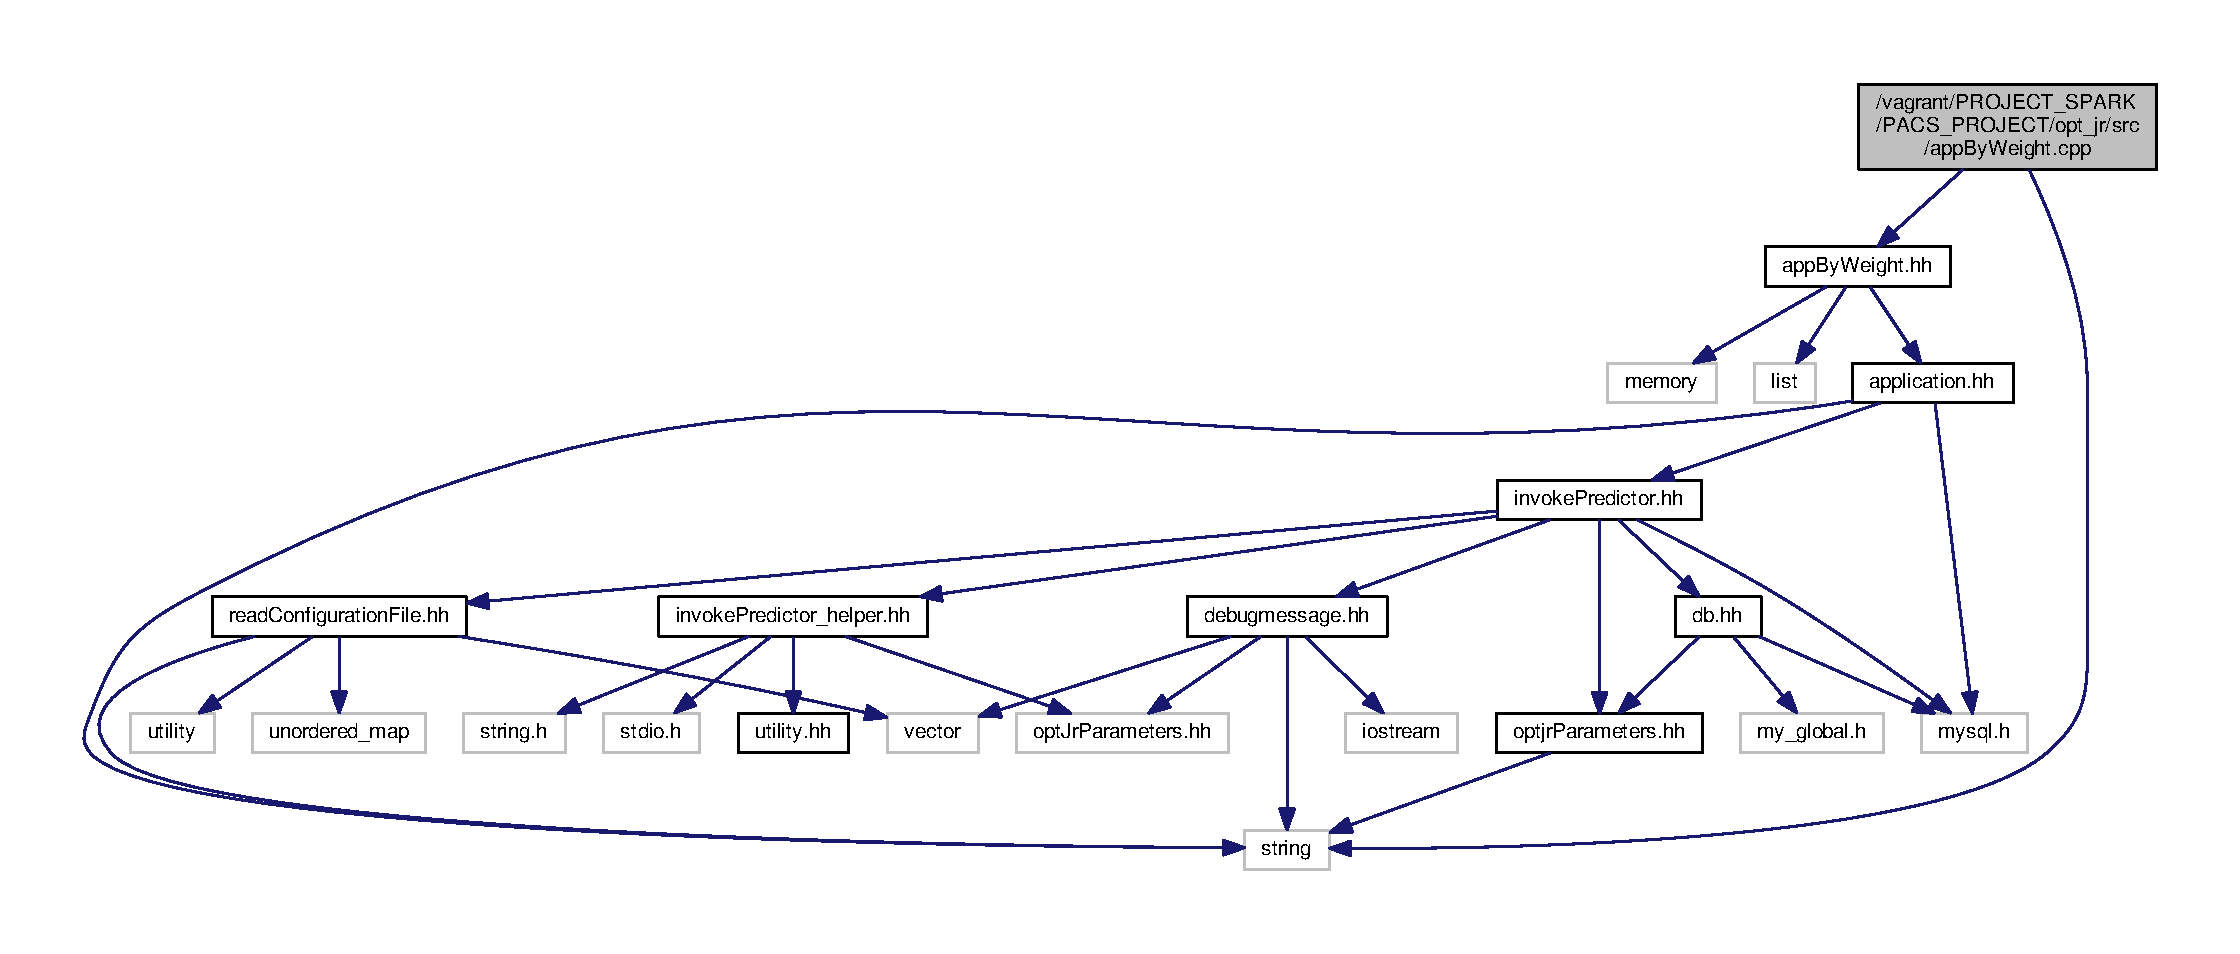
\includegraphics[width=350pt]{appByWeight_8cpp__incl}
\end{center}
\end{figure}
\subsection*{Functions}
\begin{DoxyCompactItemize}
\item 
void \hyperlink{appByWeight_8cpp_aade8f908ef9c582df27a535457f29b00}{add\-Application\-Pointer} (\hyperlink{appByWeight_8hh_a3f4c43ae502a499530745f5d622b54f1}{app\-By\-Weight} \&L\-P, \hyperlink{classApplication}{Application} \&App)
\end{DoxyCompactItemize}


\subsection{Function Documentation}
\hypertarget{appByWeight_8cpp_aade8f908ef9c582df27a535457f29b00}{\index{app\-By\-Weight.\-cpp@{app\-By\-Weight.\-cpp}!add\-Application\-Pointer@{add\-Application\-Pointer}}
\index{add\-Application\-Pointer@{add\-Application\-Pointer}!appByWeight.cpp@{app\-By\-Weight.\-cpp}}
\subsubsection[{add\-Application\-Pointer}]{\setlength{\rightskip}{0pt plus 5cm}void add\-Application\-Pointer (
\begin{DoxyParamCaption}
\item[{{\bf app\-By\-Weight} \&}]{L\-P, }
\item[{{\bf Application} \&}]{App}
\end{DoxyParamCaption}
)}}\label{appByWeight_8cpp_aade8f908ef9c582df27a535457f29b00}
It saves Application$\ast$ in decreasing weight \char`\"{}w\char`\"{} order 

Here is the caller graph for this function\-:\nopagebreak
\begin{figure}[H]
\begin{center}
\leavevmode
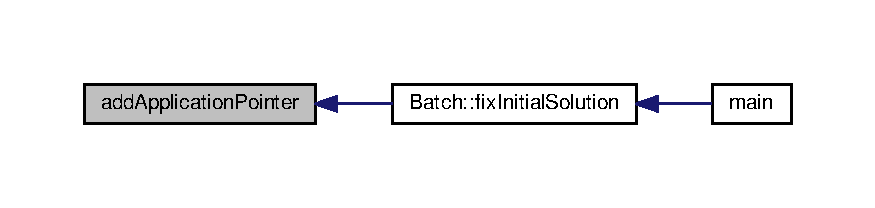
\includegraphics[width=350pt]{appByWeight_8cpp_aade8f908ef9c582df27a535457f29b00_icgraph}
\end{center}
\end{figure}



\hypertarget{appByWeight_8hh}{\section{/vagrant/\-P\-R\-O\-J\-E\-C\-T\-\_\-\-S\-P\-A\-R\-K/\-P\-A\-C\-S\-\_\-\-P\-R\-O\-J\-E\-C\-T/opt\-\_\-jr/src/app\-By\-Weight.hh File Reference}
\label{appByWeight_8hh}\index{/vagrant/\-P\-R\-O\-J\-E\-C\-T\-\_\-\-S\-P\-A\-R\-K/\-P\-A\-C\-S\-\_\-\-P\-R\-O\-J\-E\-C\-T/opt\-\_\-jr/src/app\-By\-Weight.\-hh@{/vagrant/\-P\-R\-O\-J\-E\-C\-T\-\_\-\-S\-P\-A\-R\-K/\-P\-A\-C\-S\-\_\-\-P\-R\-O\-J\-E\-C\-T/opt\-\_\-jr/src/app\-By\-Weight.\-hh}}
}
{\ttfamily \#include $<$list$>$}\\*
{\ttfamily \#include $<$memory$>$}\\*
{\ttfamily \#include \char`\"{}application.\-hh\char`\"{}}\\*
Include dependency graph for app\-By\-Weight.\-hh\-:\nopagebreak
\begin{figure}[H]
\begin{center}
\leavevmode
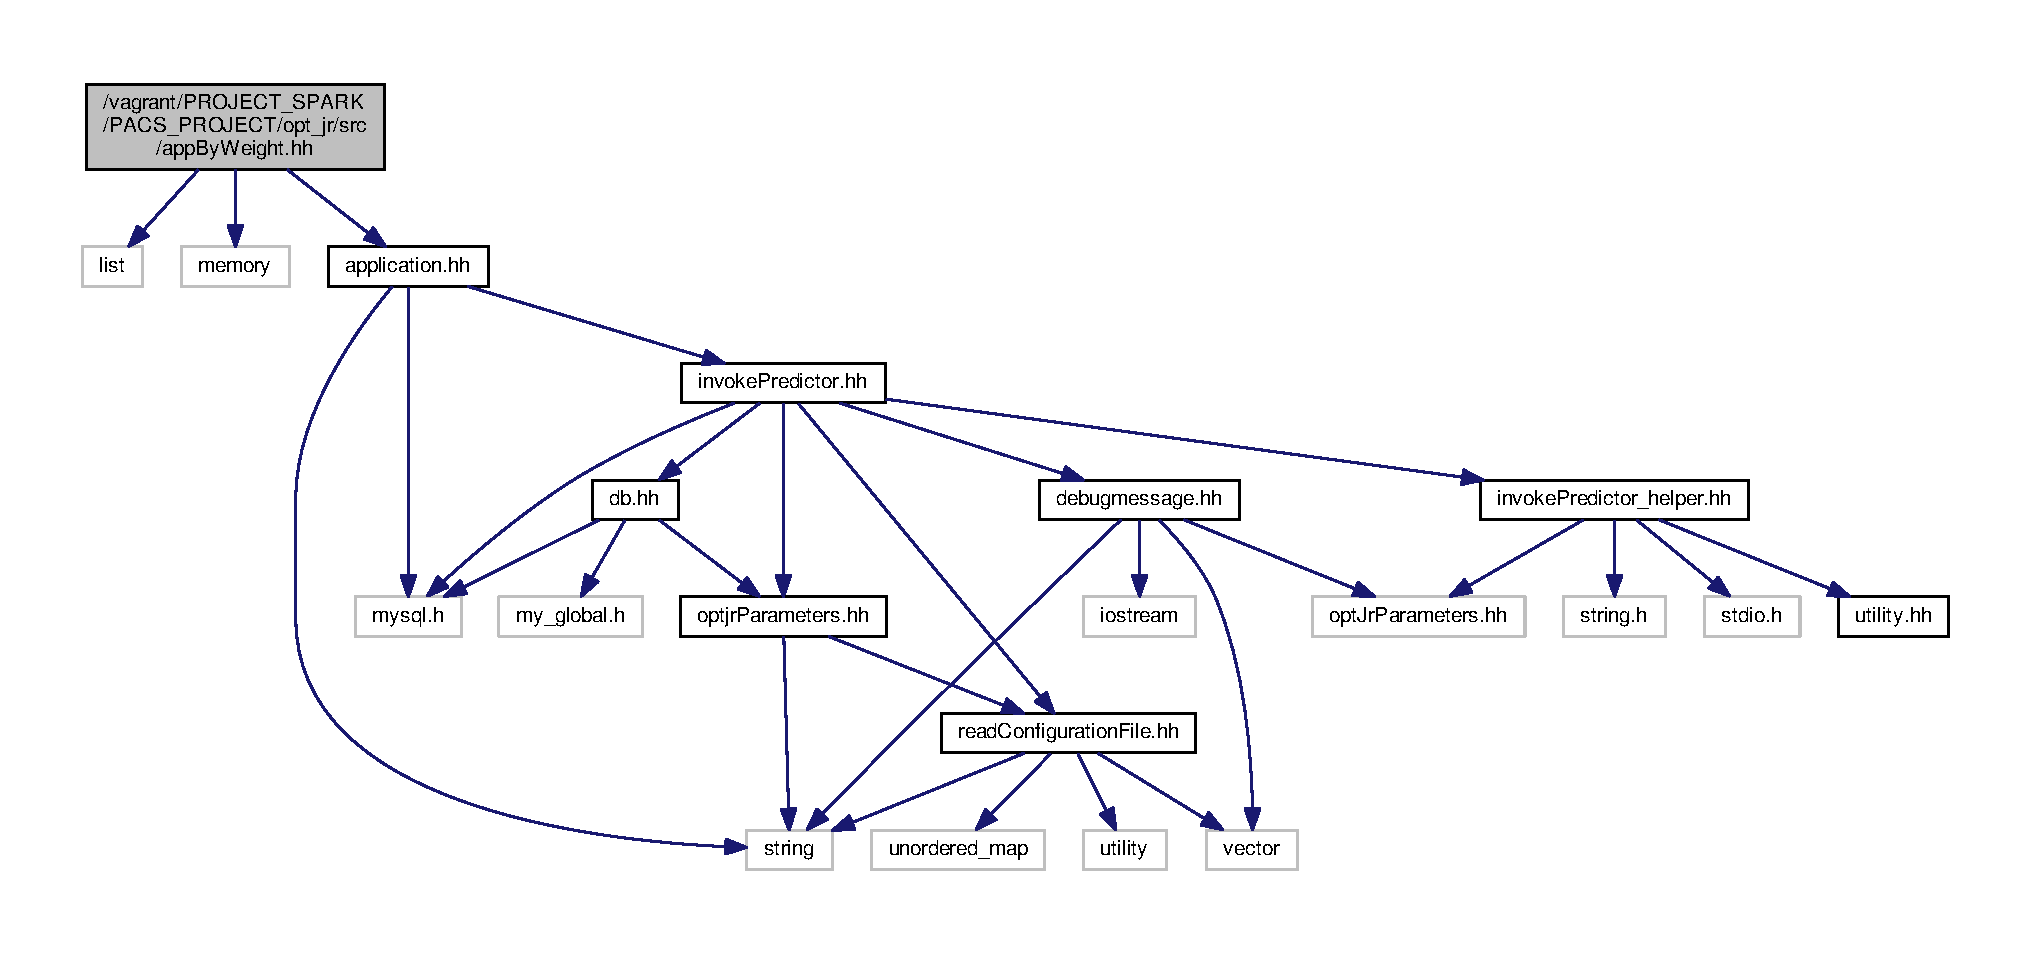
\includegraphics[width=350pt]{appByWeight_8hh__incl}
\end{center}
\end{figure}
This graph shows which files directly or indirectly include this file\-:\nopagebreak
\begin{figure}[H]
\begin{center}
\leavevmode
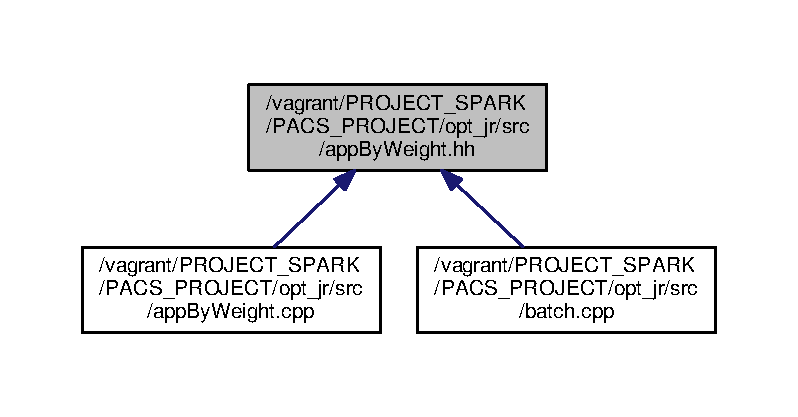
\includegraphics[width=350pt]{appByWeight_8hh__dep__incl}
\end{center}
\end{figure}
\subsection*{Typedefs}
\begin{DoxyCompactItemize}
\item 
using \hyperlink{appByWeight_8hh_a3f4c43ae502a499530745f5d622b54f1}{app\-By\-Weight} = std\-::list$<$ \hyperlink{classApplication}{Application} $\ast$ $>$
\end{DoxyCompactItemize}
\subsection*{Functions}
\begin{DoxyCompactItemize}
\item 
void \hyperlink{appByWeight_8hh_aade8f908ef9c582df27a535457f29b00}{add\-Application\-Pointer} (\hyperlink{appByWeight_8hh_a3f4c43ae502a499530745f5d622b54f1}{app\-By\-Weight} \&L\-P, \hyperlink{classApplication}{Application} \&App)
\end{DoxyCompactItemize}


\subsection{Typedef Documentation}
\hypertarget{appByWeight_8hh_a3f4c43ae502a499530745f5d622b54f1}{\index{app\-By\-Weight.\-hh@{app\-By\-Weight.\-hh}!app\-By\-Weight@{app\-By\-Weight}}
\index{app\-By\-Weight@{app\-By\-Weight}!appByWeight.hh@{app\-By\-Weight.\-hh}}
\subsubsection[{app\-By\-Weight}]{\setlength{\rightskip}{0pt plus 5cm}using {\bf app\-By\-Weight} =  std\-::list$<$ {\bf Application}$\ast$ $>$}}\label{appByWeight_8hh_a3f4c43ae502a499530745f5d622b54f1}
app\-By\-Weight is an auxiliary list of Application$\ast$ used by fix\-Initial\-Solution; through the add\-Application\-Pointer it stores Application$\ast$ ordered by weight \char`\"{}w\char`\"{} 

\subsection{Function Documentation}
\hypertarget{appByWeight_8hh_aade8f908ef9c582df27a535457f29b00}{\index{app\-By\-Weight.\-hh@{app\-By\-Weight.\-hh}!add\-Application\-Pointer@{add\-Application\-Pointer}}
\index{add\-Application\-Pointer@{add\-Application\-Pointer}!appByWeight.hh@{app\-By\-Weight.\-hh}}
\subsubsection[{add\-Application\-Pointer}]{\setlength{\rightskip}{0pt plus 5cm}void add\-Application\-Pointer (
\begin{DoxyParamCaption}
\item[{{\bf app\-By\-Weight} \&}]{L\-P, }
\item[{{\bf Application} \&}]{App}
\end{DoxyParamCaption}
)}}\label{appByWeight_8hh_aade8f908ef9c582df27a535457f29b00}
It saves Application$\ast$ in decreasing weight \char`\"{}w\char`\"{} order 

Here is the caller graph for this function\-:\nopagebreak
\begin{figure}[H]
\begin{center}
\leavevmode
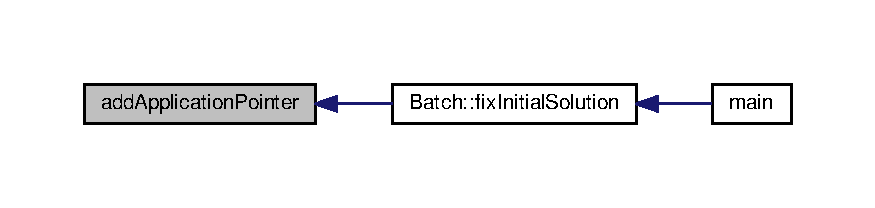
\includegraphics[width=350pt]{appByWeight_8hh_aade8f908ef9c582df27a535457f29b00_icgraph}
\end{center}
\end{figure}



\hypertarget{application_8cpp}{\section{/vagrant/\-P\-R\-O\-J\-E\-C\-T\-\_\-\-S\-P\-A\-R\-K/\-P\-A\-C\-S\-\_\-\-P\-R\-O\-J\-E\-C\-T/opt\-\_\-jr/src/application.cpp File Reference}
\label{application_8cpp}\index{/vagrant/\-P\-R\-O\-J\-E\-C\-T\-\_\-\-S\-P\-A\-R\-K/\-P\-A\-C\-S\-\_\-\-P\-R\-O\-J\-E\-C\-T/opt\-\_\-jr/src/application.\-cpp@{/vagrant/\-P\-R\-O\-J\-E\-C\-T\-\_\-\-S\-P\-A\-R\-K/\-P\-A\-C\-S\-\_\-\-P\-R\-O\-J\-E\-C\-T/opt\-\_\-jr/src/application.\-cpp}}
}
{\ttfamily \#include \char`\"{}application.\-hh\char`\"{}}\\*
Include dependency graph for application.\-cpp\-:
\nopagebreak
\begin{figure}[H]
\begin{center}
\leavevmode
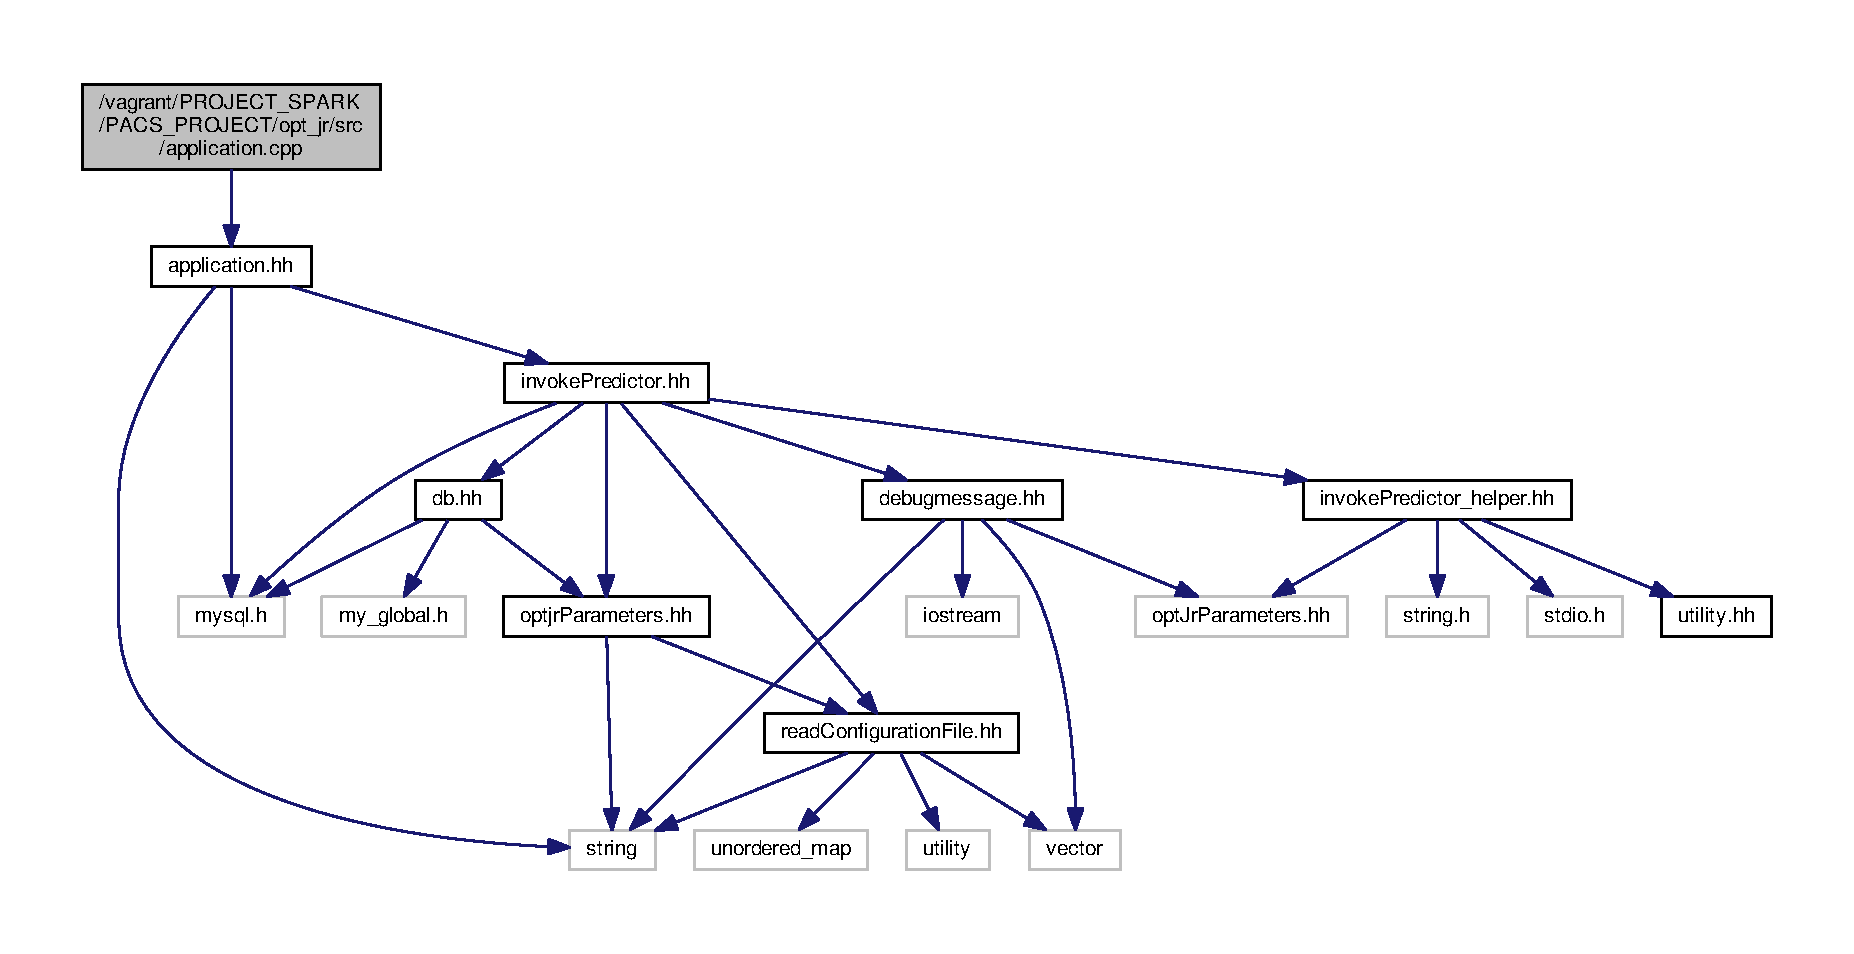
\includegraphics[width=222pt]{application_8cpp__incl}
\end{center}
\end{figure}

\hypertarget{application_8hh}{\section{/vagrant/\-P\-R\-O\-J\-E\-C\-T\-\_\-\-S\-P\-A\-R\-K/\-P\-A\-C\-S\-\_\-\-P\-R\-O\-J\-E\-C\-T/opt\-\_\-jr/src/application.hh File Reference}
\label{application_8hh}\index{/vagrant/\-P\-R\-O\-J\-E\-C\-T\-\_\-\-S\-P\-A\-R\-K/\-P\-A\-C\-S\-\_\-\-P\-R\-O\-J\-E\-C\-T/opt\-\_\-jr/src/application.\-hh@{/vagrant/\-P\-R\-O\-J\-E\-C\-T\-\_\-\-S\-P\-A\-R\-K/\-P\-A\-C\-S\-\_\-\-P\-R\-O\-J\-E\-C\-T/opt\-\_\-jr/src/application.\-hh}}
}
{\ttfamily \#include $<$string$>$}\\*
{\ttfamily \#include $<$mysql.\-h$>$}\\*
{\ttfamily \#include \char`\"{}invoke\-Predictor.\-hh\char`\"{}}\\*
Include dependency graph for application.\-hh\-:
\nopagebreak
\begin{figure}[H]
\begin{center}
\leavevmode
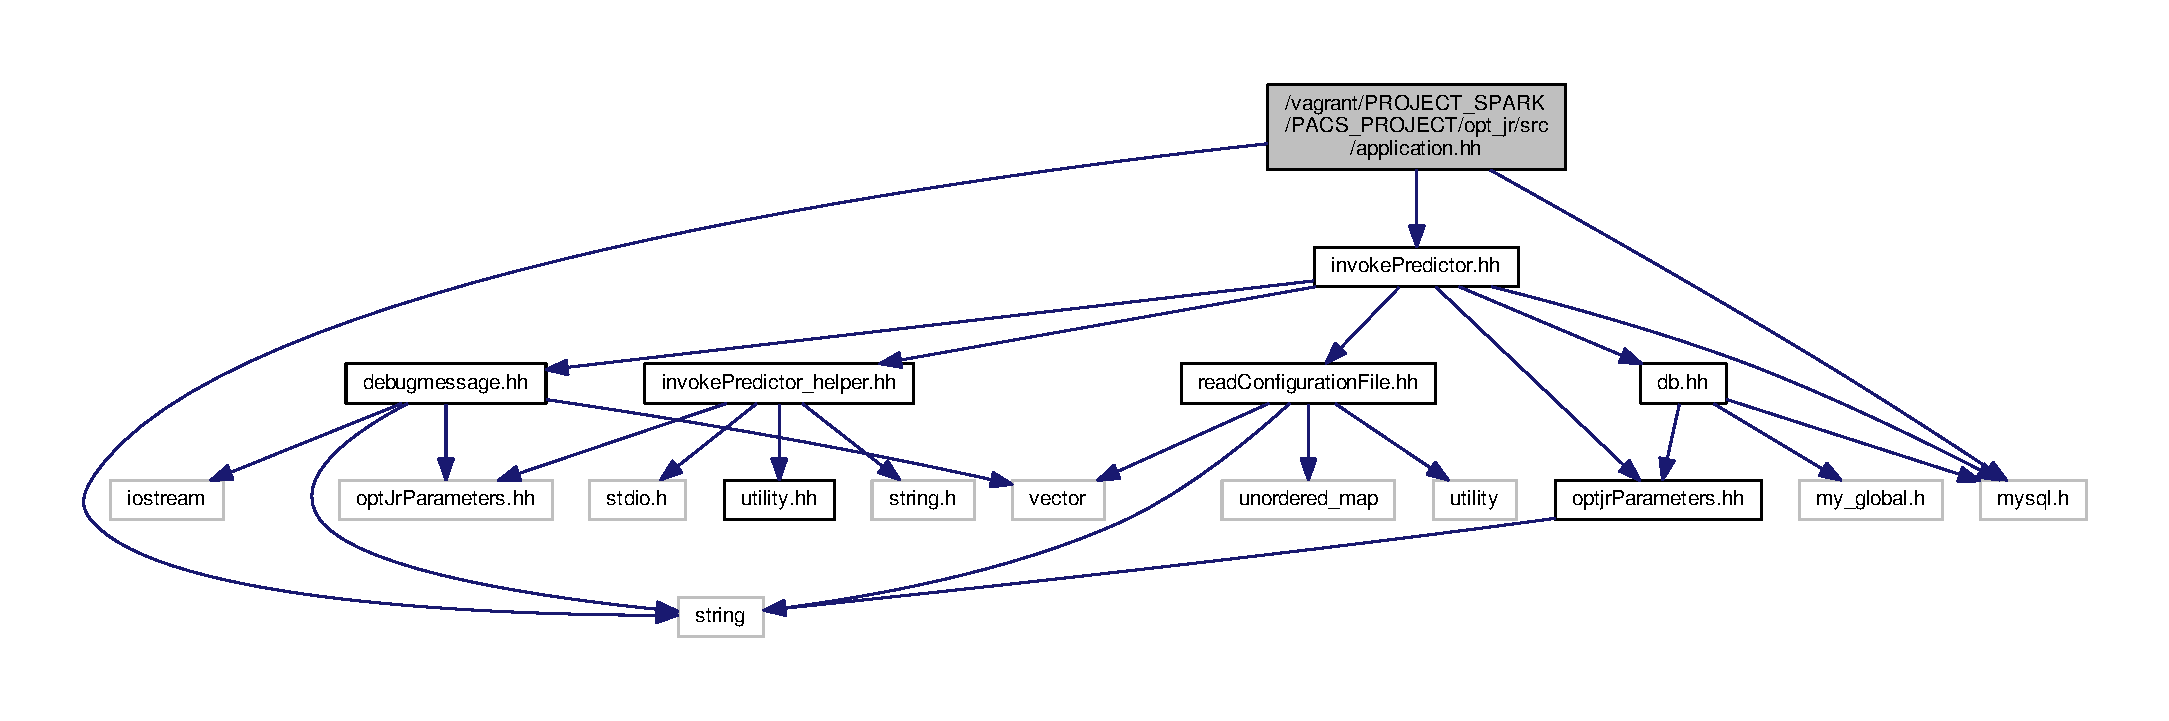
\includegraphics[width=350pt]{application_8hh__incl}
\end{center}
\end{figure}
This graph shows which files directly or indirectly include this file\-:
\nopagebreak
\begin{figure}[H]
\begin{center}
\leavevmode
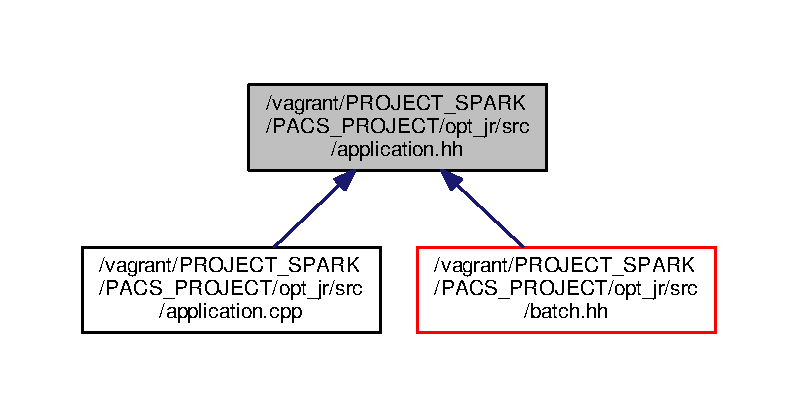
\includegraphics[width=350pt]{application_8hh__dep__incl}
\end{center}
\end{figure}
\subsection*{Classes}
\begin{DoxyCompactItemize}
\item 
class \hyperlink{classApplication}{Application}
\end{DoxyCompactItemize}
\subsection*{Macros}
\begin{DoxyCompactItemize}
\item 
\#define \hyperlink{application_8hh_aaeed326368abd712225f9ca34c338fbf}{R\-\_\-\-A\-L\-G\-O\-R\-I\-T\-H\-M}~0
\end{DoxyCompactItemize}


\subsection{Macro Definition Documentation}
\hypertarget{application_8hh_aaeed326368abd712225f9ca34c338fbf}{\index{application.\-hh@{application.\-hh}!R\-\_\-\-A\-L\-G\-O\-R\-I\-T\-H\-M@{R\-\_\-\-A\-L\-G\-O\-R\-I\-T\-H\-M}}
\index{R\-\_\-\-A\-L\-G\-O\-R\-I\-T\-H\-M@{R\-\_\-\-A\-L\-G\-O\-R\-I\-T\-H\-M}!application.hh@{application.\-hh}}
\subsubsection[{R\-\_\-\-A\-L\-G\-O\-R\-I\-T\-H\-M}]{\setlength{\rightskip}{0pt plus 5cm}\#define R\-\_\-\-A\-L\-G\-O\-R\-I\-T\-H\-M~0}}\label{application_8hh_aaeed326368abd712225f9ca34c338fbf}

\hypertarget{batch_8cpp}{\section{/vagrant/\-P\-R\-O\-J\-E\-C\-T\-\_\-\-S\-P\-A\-R\-K/\-P\-A\-C\-S\-\_\-\-P\-R\-O\-J\-E\-C\-T/opt\-\_\-jr/src/batch.cpp File Reference}
\label{batch_8cpp}\index{/vagrant/\-P\-R\-O\-J\-E\-C\-T\-\_\-\-S\-P\-A\-R\-K/\-P\-A\-C\-S\-\_\-\-P\-R\-O\-J\-E\-C\-T/opt\-\_\-jr/src/batch.\-cpp@{/vagrant/\-P\-R\-O\-J\-E\-C\-T\-\_\-\-S\-P\-A\-R\-K/\-P\-A\-C\-S\-\_\-\-P\-R\-O\-J\-E\-C\-T/opt\-\_\-jr/src/batch.\-cpp}}
}
{\ttfamily \#include \char`\"{}batch.\-hh\char`\"{}}\\*
{\ttfamily \#include \char`\"{}objective\-\_\-fun.\-hh\char`\"{}}\\*
{\ttfamily \#include \char`\"{}db.\-hh\char`\"{}}\\*
{\ttfamily \#include $<$iostream$>$}\\*
{\ttfamily \#include $<$string$>$}\\*
{\ttfamily \#include $<$cmath$>$}\\*
{\ttfamily \#include $<$list$>$}\\*
Include dependency graph for batch.\-cpp\-:
\nopagebreak
\begin{figure}[H]
\begin{center}
\leavevmode
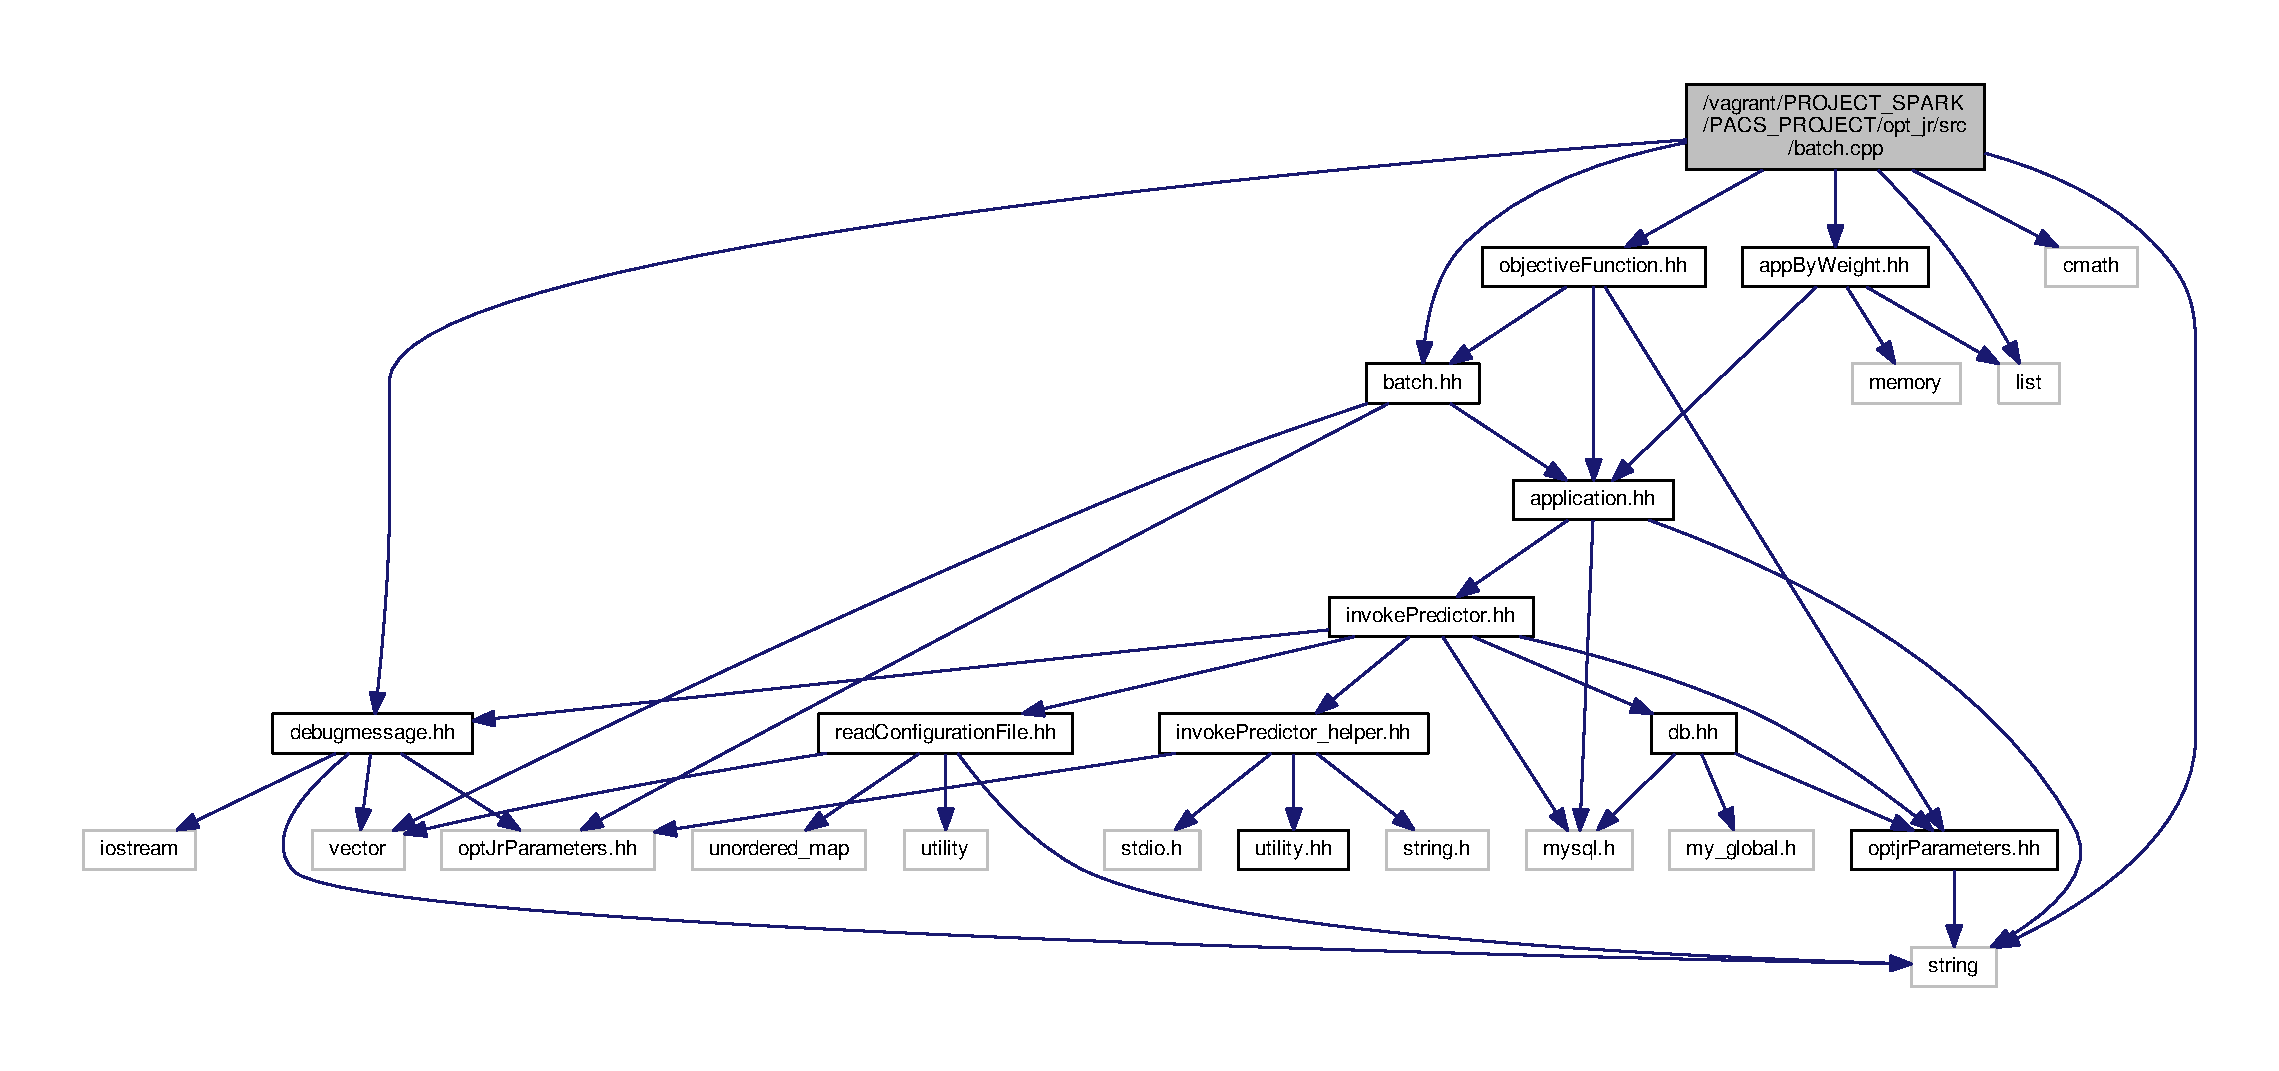
\includegraphics[width=350pt]{batch_8cpp__incl}
\end{center}
\end{figure}

\hypertarget{batch_8hh}{\section{/vagrant/\-P\-R\-O\-J\-E\-C\-T\-\_\-\-S\-P\-A\-R\-K/\-P\-A\-C\-S\-\_\-\-P\-R\-O\-J\-E\-C\-T/opt\-\_\-jr/src/batch.hh File Reference}
\label{batch_8hh}\index{/vagrant/\-P\-R\-O\-J\-E\-C\-T\-\_\-\-S\-P\-A\-R\-K/\-P\-A\-C\-S\-\_\-\-P\-R\-O\-J\-E\-C\-T/opt\-\_\-jr/src/batch.\-hh@{/vagrant/\-P\-R\-O\-J\-E\-C\-T\-\_\-\-S\-P\-A\-R\-K/\-P\-A\-C\-S\-\_\-\-P\-R\-O\-J\-E\-C\-T/opt\-\_\-jr/src/batch.\-hh}}
}
{\ttfamily \#include $<$vector$>$}\\*
{\ttfamily \#include \char`\"{}opt\-Jr\-Parameters.\-hh\char`\"{}}\\*
{\ttfamily \#include \char`\"{}application.\-hh\char`\"{}}\\*
Include dependency graph for batch.\-hh\-:
\nopagebreak
\begin{figure}[H]
\begin{center}
\leavevmode
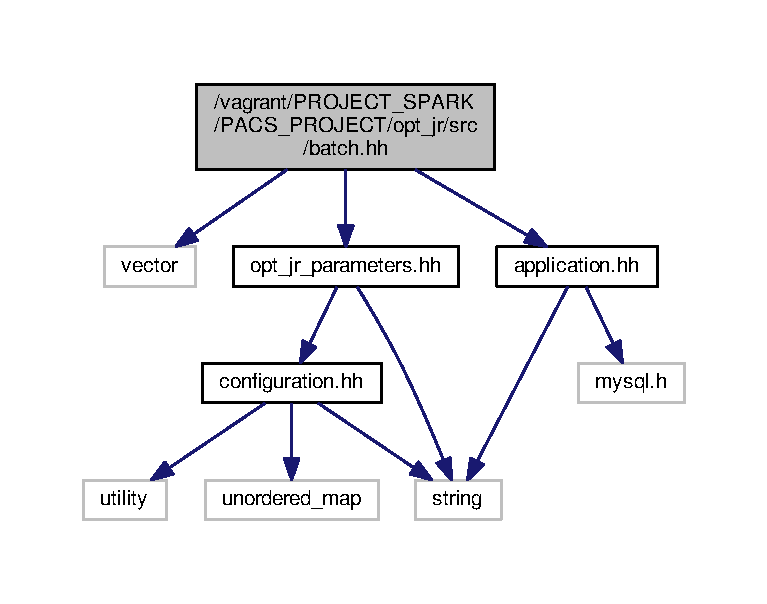
\includegraphics[width=350pt]{batch_8hh__incl}
\end{center}
\end{figure}
This graph shows which files directly or indirectly include this file\-:
\nopagebreak
\begin{figure}[H]
\begin{center}
\leavevmode
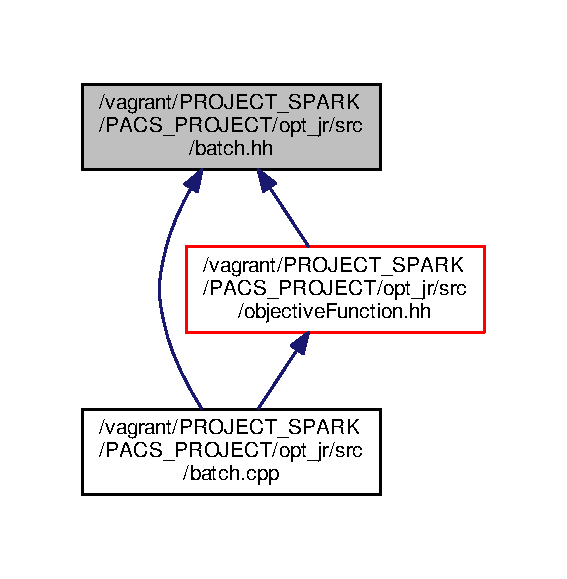
\includegraphics[width=350pt]{batch_8hh__dep__incl}
\end{center}
\end{figure}
\subsection*{Classes}
\begin{DoxyCompactItemize}
\item 
class \hyperlink{classBatch}{Batch}
\end{DoxyCompactItemize}

\hypertarget{bounds_8cpp}{\section{/vagrant/\-P\-R\-O\-J\-E\-C\-T\-\_\-\-S\-P\-A\-R\-K/\-P\-A\-C\-S\-\_\-\-P\-R\-O\-J\-E\-C\-T/opt\-\_\-jr/src/bounds.cpp File Reference}
\label{bounds_8cpp}\index{/vagrant/\-P\-R\-O\-J\-E\-C\-T\-\_\-\-S\-P\-A\-R\-K/\-P\-A\-C\-S\-\_\-\-P\-R\-O\-J\-E\-C\-T/opt\-\_\-jr/src/bounds.\-cpp@{/vagrant/\-P\-R\-O\-J\-E\-C\-T\-\_\-\-S\-P\-A\-R\-K/\-P\-A\-C\-S\-\_\-\-P\-R\-O\-J\-E\-C\-T/opt\-\_\-jr/src/bounds.\-cpp}}
}
{\ttfamily \#include \char`\"{}bounds.\-hh\char`\"{}}\\*
{\ttfamily \#include \char`\"{}debugmessage.\-hh\char`\"{}}\\*
{\ttfamily \#include \char`\"{}db.\-hh\char`\"{}}\\*
{\ttfamily \#include \char`\"{}invoke\-Predictor.\-hh\char`\"{}}\\*
{\ttfamily \#include $<$omp.\-h$>$}\\*
{\ttfamily \#include $<$math.\-h$>$}\\*

\hypertarget{bounds_8hh}{\section{/vagrant/\-P\-R\-O\-J\-E\-C\-T\-\_\-\-S\-P\-A\-R\-K/\-P\-A\-C\-S\-\_\-\-P\-R\-O\-J\-E\-C\-T/opt\-\_\-jr/src/bounds.hh File Reference}
\label{bounds_8hh}\index{/vagrant/\-P\-R\-O\-J\-E\-C\-T\-\_\-\-S\-P\-A\-R\-K/\-P\-A\-C\-S\-\_\-\-P\-R\-O\-J\-E\-C\-T/opt\-\_\-jr/src/bounds.\-hh@{/vagrant/\-P\-R\-O\-J\-E\-C\-T\-\_\-\-S\-P\-A\-R\-K/\-P\-A\-C\-S\-\_\-\-P\-R\-O\-J\-E\-C\-T/opt\-\_\-jr/src/bounds.\-hh}}
}
{\ttfamily \#include \char`\"{}batch.\-hh\char`\"{}}\\*
{\ttfamily \#include \char`\"{}read\-Configuration\-File.\-hh\char`\"{}}\\*
{\ttfamily \#include \char`\"{}optjrparameters.\-hh\char`\"{}}\\*
{\ttfamily \#include $<$mysql.\-h$>$}\\*
{\ttfamily \#include $<$string.\-h$>$}\\*
This graph shows which files directly or indirectly include this file\-:\nopagebreak
\begin{figure}[H]
\begin{center}
\leavevmode
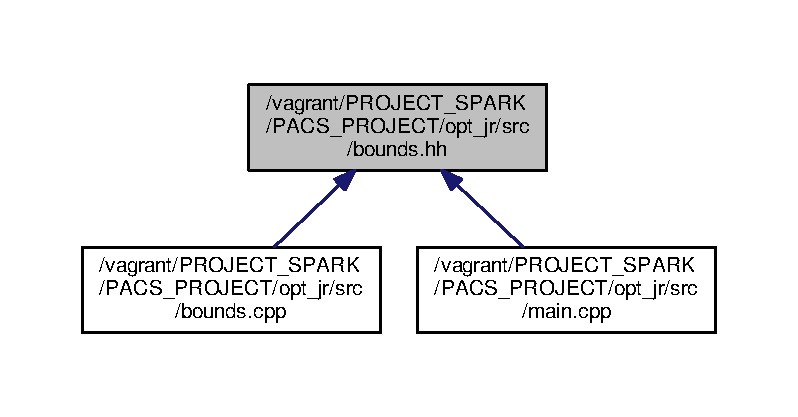
\includegraphics[width=350pt]{bounds_8hh__dep__incl}
\end{center}
\end{figure}
\subsection*{Classes}
\begin{DoxyCompactItemize}
\item 
class \hyperlink{classBounds}{Bounds}
\end{DoxyCompactItemize}

\hypertarget{candidates_8cpp}{\section{/vagrant/\-P\-R\-O\-J\-E\-C\-T\-\_\-\-S\-P\-A\-R\-K/\-P\-A\-C\-S\-\_\-\-P\-R\-O\-J\-E\-C\-T/opt\-\_\-jr/src/candidates.cpp File Reference}
\label{candidates_8cpp}\index{/vagrant/\-P\-R\-O\-J\-E\-C\-T\-\_\-\-S\-P\-A\-R\-K/\-P\-A\-C\-S\-\_\-\-P\-R\-O\-J\-E\-C\-T/opt\-\_\-jr/src/candidates.\-cpp@{/vagrant/\-P\-R\-O\-J\-E\-C\-T\-\_\-\-S\-P\-A\-R\-K/\-P\-A\-C\-S\-\_\-\-P\-R\-O\-J\-E\-C\-T/opt\-\_\-jr/src/candidates.\-cpp}}
}
{\ttfamily \#include \char`\"{}candidates.\-hh\char`\"{}}\\*
{\ttfamily \#include \char`\"{}utility.\-hh\char`\"{}}\\*
Include dependency graph for candidates.\-cpp\-:\nopagebreak
\begin{figure}[H]
\begin{center}
\leavevmode
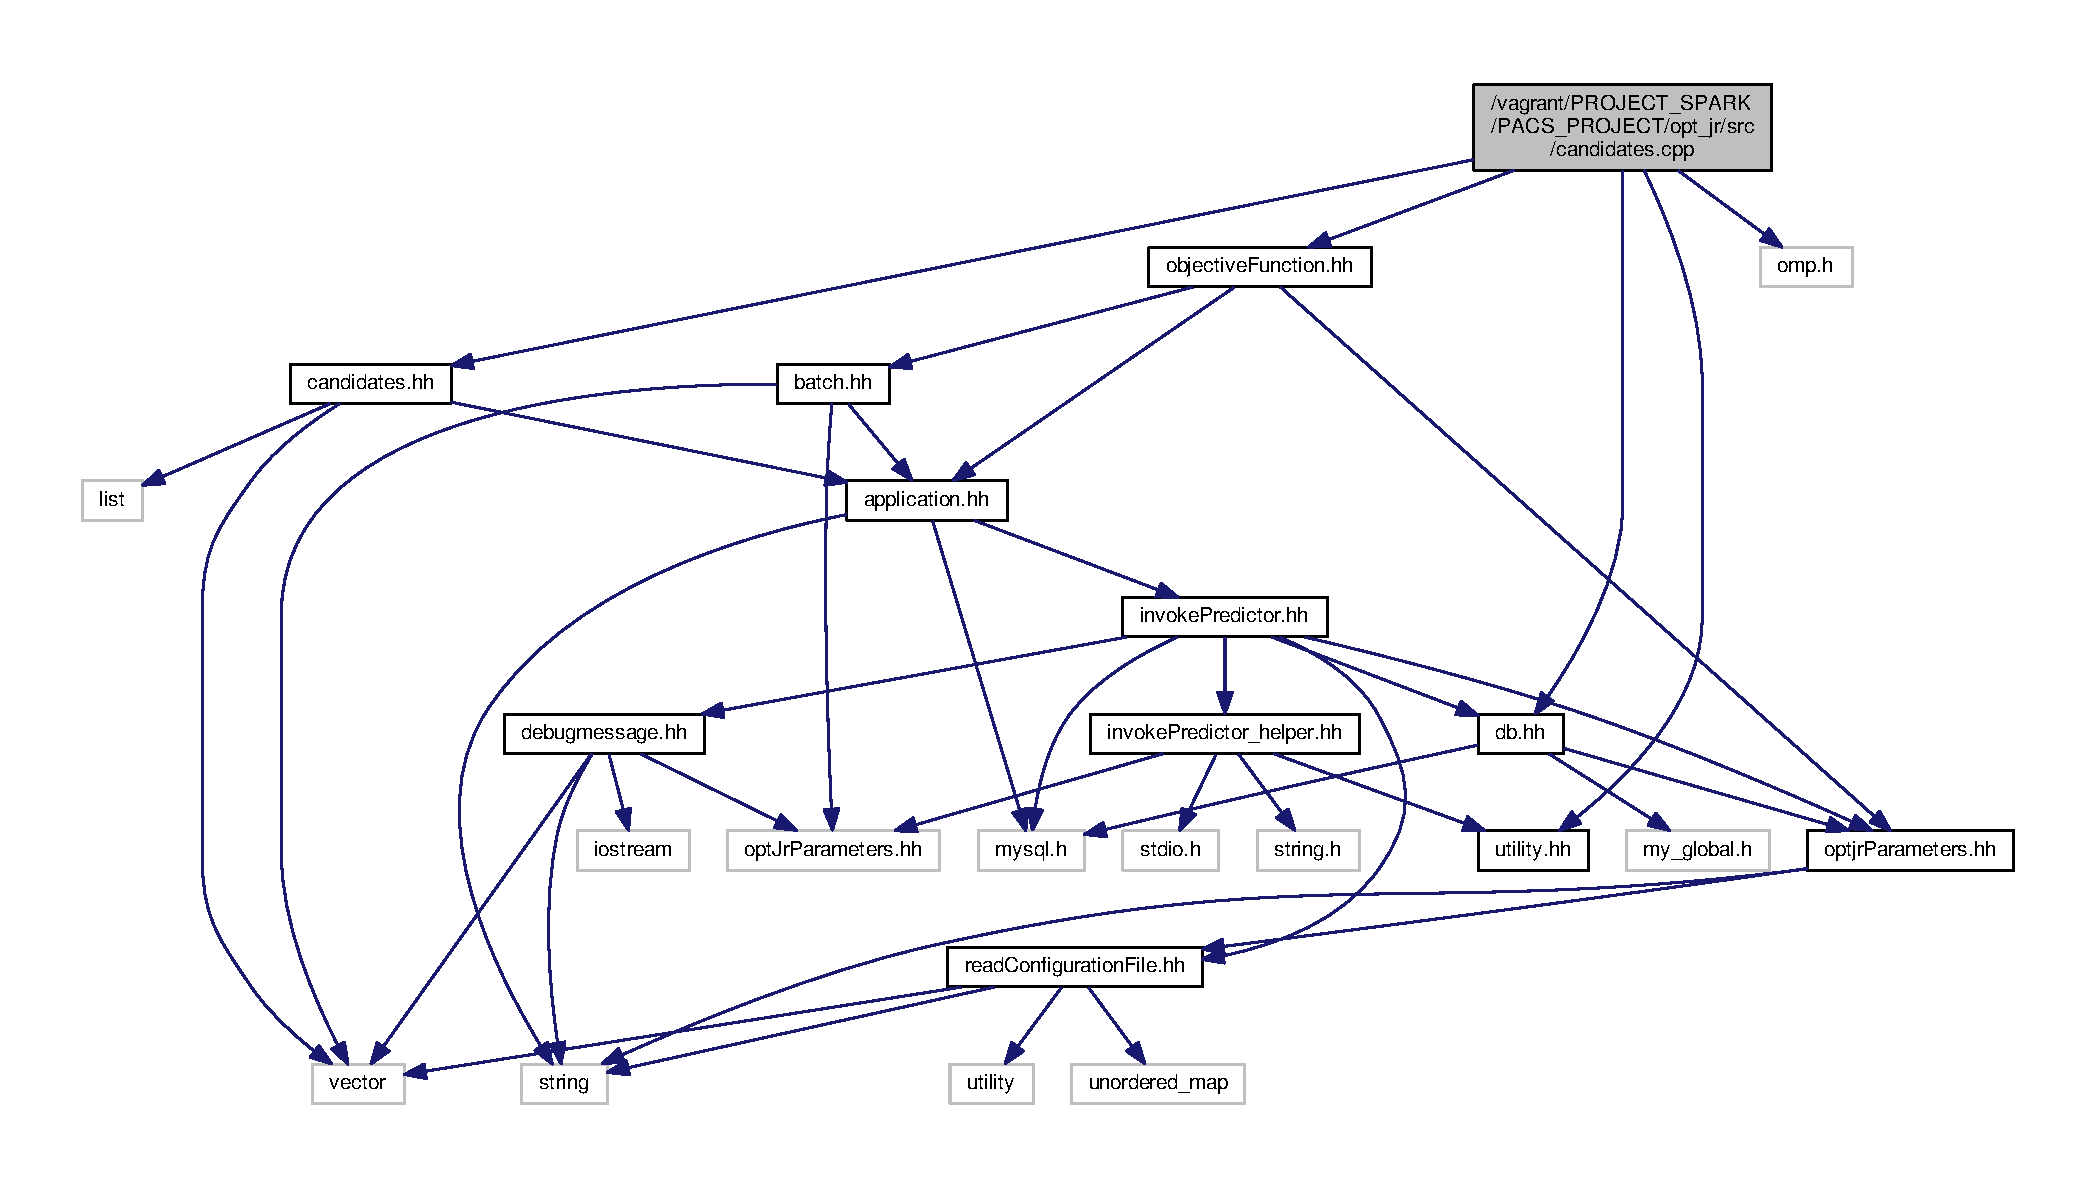
\includegraphics[width=350pt]{candidates_8cpp__incl}
\end{center}
\end{figure}
\subsection*{Functions}
\begin{DoxyCompactItemize}
\item 
void \hyperlink{candidates_8cpp_a0dead9d126fdc270fa4692dc0e4671e2}{add\-Candidate} (\hyperlink{candidates_8hh_af1ec7d668b0f7361dc7e1e1da5c4ce7d}{s\-Candidates} \&cand, \hyperlink{classApplication}{Application} \&app\-\_\-i, \hyperlink{classApplication}{Application} \&app\-\_\-j, int contr1, int contr2, double delta, double delta\-\_\-i, double delta\-\_\-j)
\end{DoxyCompactItemize}


\subsection{Function Documentation}
\hypertarget{candidates_8cpp_a0dead9d126fdc270fa4692dc0e4671e2}{\index{candidates.\-cpp@{candidates.\-cpp}!add\-Candidate@{add\-Candidate}}
\index{add\-Candidate@{add\-Candidate}!candidates.cpp@{candidates.\-cpp}}
\subsubsection[{add\-Candidate}]{\setlength{\rightskip}{0pt plus 5cm}void add\-Candidate (
\begin{DoxyParamCaption}
\item[{{\bf s\-Candidates} \&}]{cand, }
\item[{{\bf Application} \&}]{app\-\_\-i, }
\item[{{\bf Application} \&}]{app\-\_\-j, }
\item[{int}]{contr1, }
\item[{int}]{contr2, }
\item[{double}]{delta, }
\item[{double}]{delta\-\_\-i, }
\item[{double}]{delta\-\_\-j}
\end{DoxyParamCaption}
)}}\label{candidates_8cpp_a0dead9d126fdc270fa4692dc0e4671e2}


Here is the caller graph for this function\-:\nopagebreak
\begin{figure}[H]
\begin{center}
\leavevmode
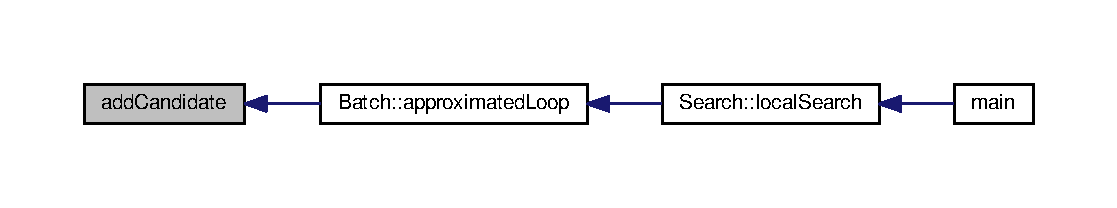
\includegraphics[width=350pt]{candidates_8cpp_a0dead9d126fdc270fa4692dc0e4671e2_icgraph}
\end{center}
\end{figure}



\hypertarget{candidates_8hh}{\section{/vagrant/\-P\-R\-O\-J\-E\-C\-T\-\_\-\-S\-P\-A\-R\-K/\-P\-A\-C\-S\-\_\-\-P\-R\-O\-J\-E\-C\-T/opt\-\_\-jr/src/candidates.hh File Reference}
\label{candidates_8hh}\index{/vagrant/\-P\-R\-O\-J\-E\-C\-T\-\_\-\-S\-P\-A\-R\-K/\-P\-A\-C\-S\-\_\-\-P\-R\-O\-J\-E\-C\-T/opt\-\_\-jr/src/candidates.\-hh@{/vagrant/\-P\-R\-O\-J\-E\-C\-T\-\_\-\-S\-P\-A\-R\-K/\-P\-A\-C\-S\-\_\-\-P\-R\-O\-J\-E\-C\-T/opt\-\_\-jr/src/candidates.\-hh}}
}
{\ttfamily \#include $<$list$>$}\\*
{\ttfamily \#include $<$vector$>$}\\*
{\ttfamily \#include \char`\"{}application.\-hh\char`\"{}}\\*
This graph shows which files directly or indirectly include this file\-:\nopagebreak
\begin{figure}[H]
\begin{center}
\leavevmode
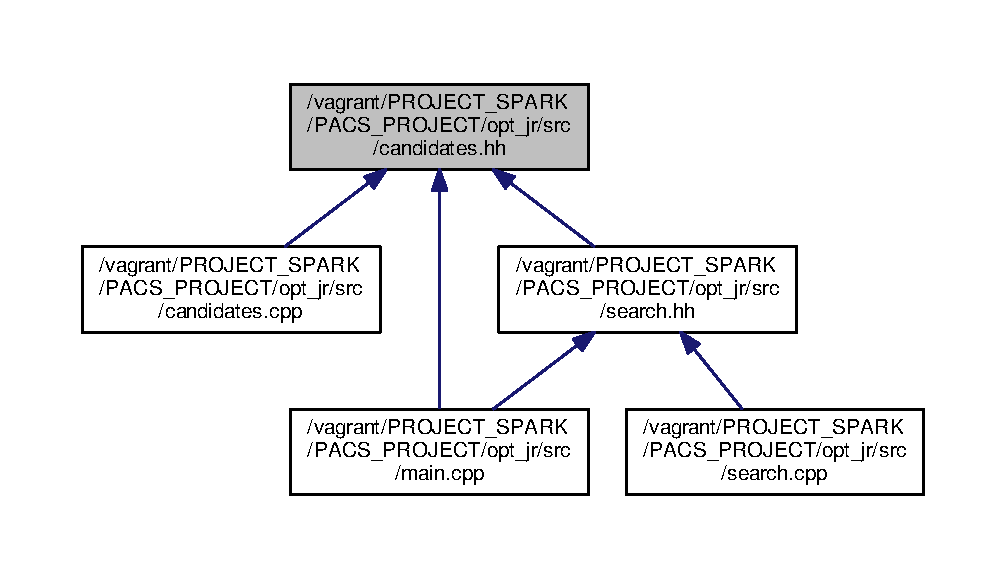
\includegraphics[width=350pt]{candidates_8hh__dep__incl}
\end{center}
\end{figure}
\subsection*{Classes}
\begin{DoxyCompactItemize}
\item 
class \hyperlink{classCandidate}{Candidate}
\item 
class \hyperlink{classsCandidates}{s\-Candidates}
\end{DoxyCompactItemize}

\hypertarget{db_8cpp}{\section{/vagrant/\-P\-R\-O\-J\-E\-C\-T\-\_\-\-S\-P\-A\-R\-K/\-P\-A\-C\-S\-\_\-\-P\-R\-O\-J\-E\-C\-T/opt\-\_\-jr/src/db.cpp File Reference}
\label{db_8cpp}\index{/vagrant/\-P\-R\-O\-J\-E\-C\-T\-\_\-\-S\-P\-A\-R\-K/\-P\-A\-C\-S\-\_\-\-P\-R\-O\-J\-E\-C\-T/opt\-\_\-jr/src/db.\-cpp@{/vagrant/\-P\-R\-O\-J\-E\-C\-T\-\_\-\-S\-P\-A\-R\-K/\-P\-A\-C\-S\-\_\-\-P\-R\-O\-J\-E\-C\-T/opt\-\_\-jr/src/db.\-cpp}}
}
{\ttfamily \#include $<$stdio.\-h$>$}\\*
{\ttfamily \#include $<$string.\-h$>$}\\*
{\ttfamily \#include $<$string$>$}\\*
{\ttfamily \#include \char`\"{}db.\-hh\char`\"{}}\\*
{\ttfamily \#include \char`\"{}debugmessage.\-hh\char`\"{}}\\*
\subsection*{Functions}
\begin{DoxyCompactItemize}
\item 
void \hyperlink{db_8cpp_ab33dd75bdc4f92249542a2bb81b343fd}{D\-Berror} (M\-Y\-S\-Q\-L $\ast$conn, char $\ast$msg)
\item 
M\-Y\-S\-Q\-L\-\_\-\-R\-O\-W \hyperlink{db_8cpp_a2491baf1bdfde4dc81303042399a6278}{execute\-S\-Q\-L} (M\-Y\-S\-Q\-L $\ast$conn, char $\ast$statement, \hyperlink{classoptJrParameters}{opt\-Jr\-Parameters} par)
\item 
M\-Y\-S\-Q\-L $\ast$ \hyperlink{db_8cpp_aced0f518cdbba35b17b3ce9f316131ce}{D\-Bopen} (char $\ast$host, char $\ast$port, char $\ast$login, char $\ast$passw, char $\ast$db\-Name)
\item 
void \hyperlink{db_8cpp_a54af21d55b55bae7b63cb28d3cd05758}{D\-Bclose} (M\-Y\-S\-Q\-L $\ast$conn)
\end{DoxyCompactItemize}


\subsection{Function Documentation}
\hypertarget{db_8cpp_a54af21d55b55bae7b63cb28d3cd05758}{\index{db.\-cpp@{db.\-cpp}!D\-Bclose@{D\-Bclose}}
\index{D\-Bclose@{D\-Bclose}!db.cpp@{db.\-cpp}}
\subsubsection[{D\-Bclose}]{\setlength{\rightskip}{0pt plus 5cm}void D\-Bclose (
\begin{DoxyParamCaption}
\item[{M\-Y\-S\-Q\-L $\ast$}]{conn}
\end{DoxyParamCaption}
)}}\label{db_8cpp_a54af21d55b55bae7b63cb28d3cd05758}
Close D\-B connection (not substantially changed from original C version) \hypertarget{db_8cpp_ab33dd75bdc4f92249542a2bb81b343fd}{\index{db.\-cpp@{db.\-cpp}!D\-Berror@{D\-Berror}}
\index{D\-Berror@{D\-Berror}!db.cpp@{db.\-cpp}}
\subsubsection[{D\-Berror}]{\setlength{\rightskip}{0pt plus 5cm}void D\-Berror (
\begin{DoxyParamCaption}
\item[{M\-Y\-S\-Q\-L $\ast$}]{conn, }
\item[{char $\ast$}]{msg}
\end{DoxyParamCaption}
)}}\label{db_8cpp_ab33dd75bdc4f92249542a2bb81b343fd}
Standard error procedure for D\-B operations (not substantially changed from original C version) \hypertarget{db_8cpp_aced0f518cdbba35b17b3ce9f316131ce}{\index{db.\-cpp@{db.\-cpp}!D\-Bopen@{D\-Bopen}}
\index{D\-Bopen@{D\-Bopen}!db.cpp@{db.\-cpp}}
\subsubsection[{D\-Bopen}]{\setlength{\rightskip}{0pt plus 5cm}M\-Y\-S\-Q\-L$\ast$ D\-Bopen (
\begin{DoxyParamCaption}
\item[{char $\ast$}]{host, }
\item[{char $\ast$}]{port, }
\item[{char $\ast$}]{login, }
\item[{char $\ast$}]{passw, }
\item[{char $\ast$}]{db\-Name}
\end{DoxyParamCaption}
)}}\label{db_8cpp_aced0f518cdbba35b17b3ce9f316131ce}
Open a D\-B connection (not substantially changed from original C version) 

Here is the call graph for this function\-:\nopagebreak
\begin{figure}[H]
\begin{center}
\leavevmode
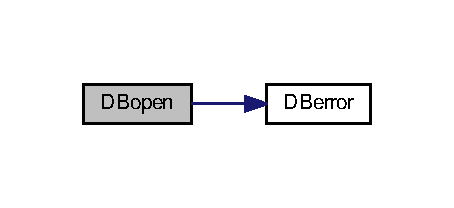
\includegraphics[width=218pt]{db_8cpp_aced0f518cdbba35b17b3ce9f316131ce_cgraph}
\end{center}
\end{figure}


\hypertarget{db_8cpp_a2491baf1bdfde4dc81303042399a6278}{\index{db.\-cpp@{db.\-cpp}!execute\-S\-Q\-L@{execute\-S\-Q\-L}}
\index{execute\-S\-Q\-L@{execute\-S\-Q\-L}!db.cpp@{db.\-cpp}}
\subsubsection[{execute\-S\-Q\-L}]{\setlength{\rightskip}{0pt plus 5cm}M\-Y\-S\-Q\-L\-\_\-\-R\-O\-W execute\-S\-Q\-L (
\begin{DoxyParamCaption}
\item[{M\-Y\-S\-Q\-L $\ast$}]{conn, }
\item[{char $\ast$}]{statement, }
\item[{{\bf opt\-Jr\-Parameters}}]{par}
\end{DoxyParamCaption}
)}}\label{db_8cpp_a2491baf1bdfde4dc81303042399a6278}
Execute S\-Q\-L statement (not substantially changed from original C version) 

Here is the call graph for this function\-:\nopagebreak
\begin{figure}[H]
\begin{center}
\leavevmode
\includegraphics[width=272pt]{db_8cpp_a2491baf1bdfde4dc81303042399a6278_cgraph}
\end{center}
\end{figure}



\hypertarget{db_8hh}{\section{/vagrant/\-P\-R\-O\-J\-E\-C\-T\-\_\-\-S\-P\-A\-R\-K/\-P\-A\-C\-S\-\_\-\-P\-R\-O\-J\-E\-C\-T/opt\-\_\-jr/src/db.hh File Reference}
\label{db_8hh}\index{/vagrant/\-P\-R\-O\-J\-E\-C\-T\-\_\-\-S\-P\-A\-R\-K/\-P\-A\-C\-S\-\_\-\-P\-R\-O\-J\-E\-C\-T/opt\-\_\-jr/src/db.\-hh@{/vagrant/\-P\-R\-O\-J\-E\-C\-T\-\_\-\-S\-P\-A\-R\-K/\-P\-A\-C\-S\-\_\-\-P\-R\-O\-J\-E\-C\-T/opt\-\_\-jr/src/db.\-hh}}
}
{\ttfamily \#include $<$my\-\_\-global.\-h$>$}\\*
{\ttfamily \#include $<$mysql.\-h$>$}\\*
{\ttfamily \#include \char`\"{}optjr\-Parameters.\-hh\char`\"{}}\\*
Include dependency graph for db.\-hh\-:\nopagebreak
\begin{figure}[H]
\begin{center}
\leavevmode
\includegraphics[width=350pt]{db_8hh__incl}
\end{center}
\end{figure}
This graph shows which files directly or indirectly include this file\-:\nopagebreak
\begin{figure}[H]
\begin{center}
\leavevmode
\includegraphics[width=350pt]{db_8hh__dep__incl}
\end{center}
\end{figure}
\subsection*{Functions}
\begin{DoxyCompactItemize}
\item 
void \hyperlink{db_8hh_ab33dd75bdc4f92249542a2bb81b343fd}{D\-Berror} (M\-Y\-S\-Q\-L $\ast$conn, char $\ast$msg)
\item 
M\-Y\-S\-Q\-L\-\_\-\-R\-O\-W \hyperlink{db_8hh_a2491baf1bdfde4dc81303042399a6278}{execute\-S\-Q\-L} (M\-Y\-S\-Q\-L $\ast$conn, char $\ast$statement, \hyperlink{classoptJrParameters}{opt\-Jr\-Parameters} par)
\item 
M\-Y\-S\-Q\-L $\ast$ \hyperlink{db_8hh_aced0f518cdbba35b17b3ce9f316131ce}{D\-Bopen} (char $\ast$host, char $\ast$port, char $\ast$login, char $\ast$passw, char $\ast$db\-Name)
\item 
void \hyperlink{db_8hh_a54af21d55b55bae7b63cb28d3cd05758}{D\-Bclose} (M\-Y\-S\-Q\-L $\ast$conn)
\end{DoxyCompactItemize}


\subsection{Function Documentation}
\hypertarget{db_8hh_a54af21d55b55bae7b63cb28d3cd05758}{\index{db.\-hh@{db.\-hh}!D\-Bclose@{D\-Bclose}}
\index{D\-Bclose@{D\-Bclose}!db.hh@{db.\-hh}}
\subsubsection[{D\-Bclose}]{\setlength{\rightskip}{0pt plus 5cm}void D\-Bclose (
\begin{DoxyParamCaption}
\item[{M\-Y\-S\-Q\-L $\ast$}]{conn}
\end{DoxyParamCaption}
)}}\label{db_8hh_a54af21d55b55bae7b63cb28d3cd05758}
Close D\-B connection (not substantially changed from original C version) 

Here is the caller graph for this function\-:\nopagebreak
\begin{figure}[H]
\begin{center}
\leavevmode
\includegraphics[width=350pt]{db_8hh_a54af21d55b55bae7b63cb28d3cd05758_icgraph}
\end{center}
\end{figure}


\hypertarget{db_8hh_ab33dd75bdc4f92249542a2bb81b343fd}{\index{db.\-hh@{db.\-hh}!D\-Berror@{D\-Berror}}
\index{D\-Berror@{D\-Berror}!db.hh@{db.\-hh}}
\subsubsection[{D\-Berror}]{\setlength{\rightskip}{0pt plus 5cm}void D\-Berror (
\begin{DoxyParamCaption}
\item[{M\-Y\-S\-Q\-L $\ast$}]{conn, }
\item[{char $\ast$}]{msg}
\end{DoxyParamCaption}
)}}\label{db_8hh_ab33dd75bdc4f92249542a2bb81b343fd}
Standard error procedure for D\-B operations (not substantially changed from original C version) 

Here is the caller graph for this function\-:\nopagebreak
\begin{figure}[H]
\begin{center}
\leavevmode
\includegraphics[width=350pt]{db_8hh_ab33dd75bdc4f92249542a2bb81b343fd_icgraph}
\end{center}
\end{figure}


\hypertarget{db_8hh_aced0f518cdbba35b17b3ce9f316131ce}{\index{db.\-hh@{db.\-hh}!D\-Bopen@{D\-Bopen}}
\index{D\-Bopen@{D\-Bopen}!db.hh@{db.\-hh}}
\subsubsection[{D\-Bopen}]{\setlength{\rightskip}{0pt plus 5cm}M\-Y\-S\-Q\-L$\ast$ D\-Bopen (
\begin{DoxyParamCaption}
\item[{char $\ast$}]{host, }
\item[{char $\ast$}]{port, }
\item[{char $\ast$}]{login, }
\item[{char $\ast$}]{passw, }
\item[{char $\ast$}]{db\-Name}
\end{DoxyParamCaption}
)}}\label{db_8hh_aced0f518cdbba35b17b3ce9f316131ce}
Open a D\-B connection (not substantially changed from original C version) 

Here is the call graph for this function\-:\nopagebreak
\begin{figure}[H]
\begin{center}
\leavevmode
\includegraphics[width=218pt]{db_8hh_aced0f518cdbba35b17b3ce9f316131ce_cgraph}
\end{center}
\end{figure}




Here is the caller graph for this function\-:\nopagebreak
\begin{figure}[H]
\begin{center}
\leavevmode
\includegraphics[width=350pt]{db_8hh_aced0f518cdbba35b17b3ce9f316131ce_icgraph}
\end{center}
\end{figure}


\hypertarget{db_8hh_a2491baf1bdfde4dc81303042399a6278}{\index{db.\-hh@{db.\-hh}!execute\-S\-Q\-L@{execute\-S\-Q\-L}}
\index{execute\-S\-Q\-L@{execute\-S\-Q\-L}!db.hh@{db.\-hh}}
\subsubsection[{execute\-S\-Q\-L}]{\setlength{\rightskip}{0pt plus 5cm}M\-Y\-S\-Q\-L\-\_\-\-R\-O\-W execute\-S\-Q\-L (
\begin{DoxyParamCaption}
\item[{M\-Y\-S\-Q\-L $\ast$}]{conn, }
\item[{char $\ast$}]{statement, }
\item[{{\bf opt\-Jr\-Parameters}}]{par}
\end{DoxyParamCaption}
)}}\label{db_8hh_a2491baf1bdfde4dc81303042399a6278}
Execute S\-Q\-L statement (not substantially changed from original C version) 

Here is the call graph for this function\-:\nopagebreak
\begin{figure}[H]
\begin{center}
\leavevmode
\includegraphics[width=350pt]{db_8hh_a2491baf1bdfde4dc81303042399a6278_cgraph}
\end{center}
\end{figure}




Here is the caller graph for this function\-:\nopagebreak
\begin{figure}[H]
\begin{center}
\leavevmode
\includegraphics[width=350pt]{db_8hh_a2491baf1bdfde4dc81303042399a6278_icgraph}
\end{center}
\end{figure}



\hypertarget{debugmessage_8cpp}{\section{/vagrant/\-P\-R\-O\-J\-E\-C\-T\-\_\-\-S\-P\-A\-R\-K/\-P\-A\-C\-S\-\_\-\-P\-R\-O\-J\-E\-C\-T/opt\-\_\-jr/src/debugmessage.cpp File Reference}
\label{debugmessage_8cpp}\index{/vagrant/\-P\-R\-O\-J\-E\-C\-T\-\_\-\-S\-P\-A\-R\-K/\-P\-A\-C\-S\-\_\-\-P\-R\-O\-J\-E\-C\-T/opt\-\_\-jr/src/debugmessage.\-cpp@{/vagrant/\-P\-R\-O\-J\-E\-C\-T\-\_\-\-S\-P\-A\-R\-K/\-P\-A\-C\-S\-\_\-\-P\-R\-O\-J\-E\-C\-T/opt\-\_\-jr/src/debugmessage.\-cpp}}
}
{\ttfamily \#include \char`\"{}debugmessage.\-hh\char`\"{}}\\*
Include dependency graph for debugmessage.\-cpp\-:\nopagebreak
\begin{figure}[H]
\begin{center}
\leavevmode
\includegraphics[width=350pt]{debugmessage_8cpp__incl}
\end{center}
\end{figure}
\subsection*{Functions}
\begin{DoxyCompactItemize}
\item 
void \hyperlink{debugmessage_8cpp_a7216d8ca989b1eaea79109c2a1236024}{debug\-Message} (std\-::string \&string, \hyperlink{classoptJrParameters}{opt\-Jr\-Parameters} \&par)
\end{DoxyCompactItemize}


\subsection{Function Documentation}
\hypertarget{debugmessage_8cpp_a7216d8ca989b1eaea79109c2a1236024}{\index{debugmessage.\-cpp@{debugmessage.\-cpp}!debug\-Message@{debug\-Message}}
\index{debug\-Message@{debug\-Message}!debugmessage.cpp@{debugmessage.\-cpp}}
\subsubsection[{debug\-Message}]{\setlength{\rightskip}{0pt plus 5cm}void debug\-Message (
\begin{DoxyParamCaption}
\item[{std\-::string \&}]{string, }
\item[{{\bf opt\-Jr\-Parameters} \&}]{par}
\end{DoxyParamCaption}
)}}\label{debugmessage_8cpp_a7216d8ca989b1eaea79109c2a1236024}


Here is the call graph for this function\-:\nopagebreak
\begin{figure}[H]
\begin{center}
\leavevmode
\includegraphics[width=308pt]{debugmessage_8cpp_a7216d8ca989b1eaea79109c2a1236024_cgraph}
\end{center}
\end{figure}




Here is the caller graph for this function\-:\nopagebreak
\begin{figure}[H]
\begin{center}
\leavevmode
\includegraphics[width=350pt]{debugmessage_8cpp_a7216d8ca989b1eaea79109c2a1236024_icgraph}
\end{center}
\end{figure}



\hypertarget{debugmessage_8hh}{\section{/vagrant/\-P\-R\-O\-J\-E\-C\-T\-\_\-\-S\-P\-A\-R\-K/\-P\-A\-C\-S\-\_\-\-P\-R\-O\-J\-E\-C\-T/opt\-\_\-jr/src/debugmessage.hh File Reference}
\label{debugmessage_8hh}\index{/vagrant/\-P\-R\-O\-J\-E\-C\-T\-\_\-\-S\-P\-A\-R\-K/\-P\-A\-C\-S\-\_\-\-P\-R\-O\-J\-E\-C\-T/opt\-\_\-jr/src/debugmessage.\-hh@{/vagrant/\-P\-R\-O\-J\-E\-C\-T\-\_\-\-S\-P\-A\-R\-K/\-P\-A\-C\-S\-\_\-\-P\-R\-O\-J\-E\-C\-T/opt\-\_\-jr/src/debugmessage.\-hh}}
}
{\ttfamily \#include $<$iostream$>$}\\*
{\ttfamily \#include $<$string$>$}\\*
{\ttfamily \#include $<$vector$>$}\\*
{\ttfamily \#include \char`\"{}opt\-Jr\-Parameters.\-hh\char`\"{}}\\*
Include dependency graph for debugmessage.\-hh\-:\nopagebreak
\begin{figure}[H]
\begin{center}
\leavevmode
\includegraphics[width=350pt]{debugmessage_8hh__incl}
\end{center}
\end{figure}
This graph shows which files directly or indirectly include this file\-:\nopagebreak
\begin{figure}[H]
\begin{center}
\leavevmode
\includegraphics[width=350pt]{debugmessage_8hh__dep__incl}
\end{center}
\end{figure}
\subsection*{Functions}
\begin{DoxyCompactItemize}
\item 
void \hyperlink{debugmessage_8hh_a7216d8ca989b1eaea79109c2a1236024}{debug\-Message} (std\-::string \&string, \hyperlink{classoptJrParameters}{opt\-Jr\-Parameters} \&par)
\end{DoxyCompactItemize}


\subsection{Function Documentation}
\hypertarget{debugmessage_8hh_a7216d8ca989b1eaea79109c2a1236024}{\index{debugmessage.\-hh@{debugmessage.\-hh}!debug\-Message@{debug\-Message}}
\index{debug\-Message@{debug\-Message}!debugmessage.hh@{debugmessage.\-hh}}
\subsubsection[{debug\-Message}]{\setlength{\rightskip}{0pt plus 5cm}void debug\-Message (
\begin{DoxyParamCaption}
\item[{std\-::string \&}]{string, }
\item[{{\bf opt\-Jr\-Parameters} \&}]{par}
\end{DoxyParamCaption}
)}}\label{debugmessage_8hh_a7216d8ca989b1eaea79109c2a1236024}
debug function\-: if debugging is activated it shows the message in string 

Here is the call graph for this function\-:\nopagebreak
\begin{figure}[H]
\begin{center}
\leavevmode
\includegraphics[width=308pt]{debugmessage_8hh_a7216d8ca989b1eaea79109c2a1236024_cgraph}
\end{center}
\end{figure}




Here is the caller graph for this function\-:\nopagebreak
\begin{figure}[H]
\begin{center}
\leavevmode
\includegraphics[width=350pt]{debugmessage_8hh_a7216d8ca989b1eaea79109c2a1236024_icgraph}
\end{center}
\end{figure}



\hypertarget{invokePredictor_8cpp}{\section{/vagrant/\-P\-R\-O\-J\-E\-C\-T\-\_\-\-S\-P\-A\-R\-K/\-P\-A\-C\-S\-\_\-\-P\-R\-O\-J\-E\-C\-T/opt\-\_\-jr/src/invoke\-Predictor.cpp File Reference}
\label{invokePredictor_8cpp}\index{/vagrant/\-P\-R\-O\-J\-E\-C\-T\-\_\-\-S\-P\-A\-R\-K/\-P\-A\-C\-S\-\_\-\-P\-R\-O\-J\-E\-C\-T/opt\-\_\-jr/src/invoke\-Predictor.\-cpp@{/vagrant/\-P\-R\-O\-J\-E\-C\-T\-\_\-\-S\-P\-A\-R\-K/\-P\-A\-C\-S\-\_\-\-P\-R\-O\-J\-E\-C\-T/opt\-\_\-jr/src/invoke\-Predictor.\-cpp}}
}
{\ttfamily \#include \char`\"{}invoke\-Predictor.\-hh\char`\"{}}\\*
{\ttfamily \#include $<$string$>$}\\*
{\ttfamily \#include $<$string.\-h$>$}\\*
Include dependency graph for invoke\-Predictor.\-cpp\-:\nopagebreak
\begin{figure}[H]
\begin{center}
\leavevmode
\includegraphics[width=350pt]{invokePredictor_8cpp__incl}
\end{center}
\end{figure}
\subsection*{Functions}
\begin{DoxyCompactItemize}
\item 
char $\ast$ \hyperlink{invokePredictor_8cpp_a342ccdfe7923368e52a4894d69c7455a}{invoke\-Predictor} (\hyperlink{readConfigurationFile_8hh_ab8f35b1da3261263c5e9c0e7c8921f5c}{s\-Configuration} \&configuration, M\-Y\-S\-Q\-L $\ast$conn, int n\-Nodes, int current\-Cores, char $\ast$memory, int datasize, char $\ast$session\-Id, char $\ast$app\-Id, char $\ast$stage, \hyperlink{classoptJrParameters}{opt\-Jr\-Parameters} \&par, int flag\-Dagsim)
\end{DoxyCompactItemize}


\subsection{Function Documentation}
\hypertarget{invokePredictor_8cpp_a342ccdfe7923368e52a4894d69c7455a}{\index{invoke\-Predictor.\-cpp@{invoke\-Predictor.\-cpp}!invoke\-Predictor@{invoke\-Predictor}}
\index{invoke\-Predictor@{invoke\-Predictor}!invokePredictor.cpp@{invoke\-Predictor.\-cpp}}
\subsubsection[{invoke\-Predictor}]{\setlength{\rightskip}{0pt plus 5cm}char$\ast$ invoke\-Predictor (
\begin{DoxyParamCaption}
\item[{{\bf s\-Configuration} \&}]{configuration, }
\item[{M\-Y\-S\-Q\-L $\ast$}]{conn, }
\item[{int}]{n\-Nodes, }
\item[{int}]{current\-Cores, }
\item[{char $\ast$}]{memory, }
\item[{int}]{datasize, }
\item[{char $\ast$}]{session\-Id, }
\item[{char $\ast$}]{app\-Id, }
\item[{char $\ast$}]{stage, }
\item[{{\bf opt\-Jr\-Parameters} \&}]{par, }
\item[{int}]{flag\-Dagsim}
\end{DoxyParamCaption}
)}}\label{invokePredictor_8cpp_a342ccdfe7923368e52a4894d69c7455a}
\char`\"{}invoke\-Predictor\char`\"{} invokes a predictor (dag\-Sim/\-Lundstrom). First it checks if an estimate of the execution time is already stored in the D\-B; if not, it invokes the actual predictor and stores the result on D\-B cache table. 

Here is the call graph for this function\-:\nopagebreak
\begin{figure}[H]
\begin{center}
\leavevmode
\includegraphics[width=350pt]{invokePredictor_8cpp_a342ccdfe7923368e52a4894d69c7455a_cgraph}
\end{center}
\end{figure}




Here is the caller graph for this function\-:
\nopagebreak
\begin{figure}[H]
\begin{center}
\leavevmode
\includegraphics[width=350pt]{invokePredictor_8cpp_a342ccdfe7923368e52a4894d69c7455a_icgraph}
\end{center}
\end{figure}



\hypertarget{invokePredictor_8hh}{\section{/vagrant/\-P\-R\-O\-J\-E\-C\-T\-\_\-\-S\-P\-A\-R\-K/\-P\-A\-C\-S\-\_\-\-P\-R\-O\-J\-E\-C\-T/opt\-\_\-jr/src/invoke\-Predictor.hh File Reference}
\label{invokePredictor_8hh}\index{/vagrant/\-P\-R\-O\-J\-E\-C\-T\-\_\-\-S\-P\-A\-R\-K/\-P\-A\-C\-S\-\_\-\-P\-R\-O\-J\-E\-C\-T/opt\-\_\-jr/src/invoke\-Predictor.\-hh@{/vagrant/\-P\-R\-O\-J\-E\-C\-T\-\_\-\-S\-P\-A\-R\-K/\-P\-A\-C\-S\-\_\-\-P\-R\-O\-J\-E\-C\-T/opt\-\_\-jr/src/invoke\-Predictor.\-hh}}
}
{\ttfamily \#include \char`\"{}invoke\-Predictor\-\_\-helper.\-hh\char`\"{}}\\*
{\ttfamily \#include \char`\"{}read\-Configuration\-File.\-hh\char`\"{}}\\*
{\ttfamily \#include \char`\"{}optjr\-Parameters.\-hh\char`\"{}}\\*
{\ttfamily \#include \char`\"{}debugmessage.\-hh\char`\"{}}\\*
{\ttfamily \#include \char`\"{}db.\-hh\char`\"{}}\\*
{\ttfamily \#include $<$mysql.\-h$>$}\\*
This graph shows which files directly or indirectly include this file\-:\nopagebreak
\begin{figure}[H]
\begin{center}
\leavevmode
\includegraphics[width=350pt]{invokePredictor_8hh__dep__incl}
\end{center}
\end{figure}
\subsection*{Macros}
\begin{DoxyCompactItemize}
\item 
\#define \hyperlink{invokePredictor_8hh_a3806de5f70b6971cfe8be82520f4bf2a}{W\-H\-O\-L\-E\-\_\-\-D\-A\-G\-S\-I\-M}~0
\item 
\#define \hyperlink{invokePredictor_8hh_a016c9fba38e790ceafd4d9843f2dc564}{R\-E\-S\-I\-D\-U\-A\-L\-\_\-\-D\-A\-G\-S\-I\-M}~1
\end{DoxyCompactItemize}
\subsection*{Functions}
\begin{DoxyCompactItemize}
\item 
char $\ast$ \hyperlink{invokePredictor_8hh_a342ccdfe7923368e52a4894d69c7455a}{invoke\-Predictor} (\hyperlink{readConfigurationFile_8hh_ab8f35b1da3261263c5e9c0e7c8921f5c}{s\-Configuration} \&configuration, M\-Y\-S\-Q\-L $\ast$conn, int n\-Nodes, int current\-Cores, char $\ast$memory, int datasize, char $\ast$session\-Id, char $\ast$app\-Id, char $\ast$stage, \hyperlink{classoptJrParameters}{opt\-Jr\-Parameters} \&par, int flag\-Dagsim)
\end{DoxyCompactItemize}


\subsection{Macro Definition Documentation}
\hypertarget{invokePredictor_8hh_a016c9fba38e790ceafd4d9843f2dc564}{\index{invoke\-Predictor.\-hh@{invoke\-Predictor.\-hh}!R\-E\-S\-I\-D\-U\-A\-L\-\_\-\-D\-A\-G\-S\-I\-M@{R\-E\-S\-I\-D\-U\-A\-L\-\_\-\-D\-A\-G\-S\-I\-M}}
\index{R\-E\-S\-I\-D\-U\-A\-L\-\_\-\-D\-A\-G\-S\-I\-M@{R\-E\-S\-I\-D\-U\-A\-L\-\_\-\-D\-A\-G\-S\-I\-M}!invokePredictor.hh@{invoke\-Predictor.\-hh}}
\subsubsection[{R\-E\-S\-I\-D\-U\-A\-L\-\_\-\-D\-A\-G\-S\-I\-M}]{\setlength{\rightskip}{0pt plus 5cm}\#define R\-E\-S\-I\-D\-U\-A\-L\-\_\-\-D\-A\-G\-S\-I\-M~1}}\label{invokePredictor_8hh_a016c9fba38e790ceafd4d9843f2dc564}
\hypertarget{invokePredictor_8hh_a3806de5f70b6971cfe8be82520f4bf2a}{\index{invoke\-Predictor.\-hh@{invoke\-Predictor.\-hh}!W\-H\-O\-L\-E\-\_\-\-D\-A\-G\-S\-I\-M@{W\-H\-O\-L\-E\-\_\-\-D\-A\-G\-S\-I\-M}}
\index{W\-H\-O\-L\-E\-\_\-\-D\-A\-G\-S\-I\-M@{W\-H\-O\-L\-E\-\_\-\-D\-A\-G\-S\-I\-M}!invokePredictor.hh@{invoke\-Predictor.\-hh}}
\subsubsection[{W\-H\-O\-L\-E\-\_\-\-D\-A\-G\-S\-I\-M}]{\setlength{\rightskip}{0pt plus 5cm}\#define W\-H\-O\-L\-E\-\_\-\-D\-A\-G\-S\-I\-M~0}}\label{invokePredictor_8hh_a3806de5f70b6971cfe8be82520f4bf2a}


\subsection{Function Documentation}
\hypertarget{invokePredictor_8hh_a342ccdfe7923368e52a4894d69c7455a}{\index{invoke\-Predictor.\-hh@{invoke\-Predictor.\-hh}!invoke\-Predictor@{invoke\-Predictor}}
\index{invoke\-Predictor@{invoke\-Predictor}!invokePredictor.hh@{invoke\-Predictor.\-hh}}
\subsubsection[{invoke\-Predictor}]{\setlength{\rightskip}{0pt plus 5cm}char$\ast$ invoke\-Predictor (
\begin{DoxyParamCaption}
\item[{{\bf s\-Configuration} \&}]{configuration, }
\item[{M\-Y\-S\-Q\-L $\ast$}]{conn, }
\item[{int}]{n\-Nodes, }
\item[{int}]{current\-Cores, }
\item[{char $\ast$}]{memory, }
\item[{int}]{datasize, }
\item[{char $\ast$}]{session\-Id, }
\item[{char $\ast$}]{app\-Id, }
\item[{char $\ast$}]{stage, }
\item[{{\bf opt\-Jr\-Parameters} \&}]{par, }
\item[{int}]{flag\-Dagsim}
\end{DoxyParamCaption}
)}}\label{invokePredictor_8hh_a342ccdfe7923368e52a4894d69c7455a}
\char`\"{}invoke\-Predictor\char`\"{} invokes a predictor (dag\-Sim/\-Lundstrom). First it checks if an estimate of the execution time is already stored in the D\-B; if not, it invokes the actual predictor and stores the result on D\-B cache table. 

Here is the caller graph for this function\-:\nopagebreak
\begin{figure}[H]
\begin{center}
\leavevmode
\includegraphics[width=350pt]{invokePredictor_8hh_a342ccdfe7923368e52a4894d69c7455a_icgraph}
\end{center}
\end{figure}



\hypertarget{invokePredictor__helper_8cpp}{\section{/vagrant/\-P\-R\-O\-J\-E\-C\-T\-\_\-\-S\-P\-A\-R\-K/\-P\-A\-C\-S\-\_\-\-P\-R\-O\-J\-E\-C\-T/opt\-\_\-jr/src/invoke\-Predictor\-\_\-helper.cpp File Reference}
\label{invokePredictor__helper_8cpp}\index{/vagrant/\-P\-R\-O\-J\-E\-C\-T\-\_\-\-S\-P\-A\-R\-K/\-P\-A\-C\-S\-\_\-\-P\-R\-O\-J\-E\-C\-T/opt\-\_\-jr/src/invoke\-Predictor\-\_\-helper.\-cpp@{/vagrant/\-P\-R\-O\-J\-E\-C\-T\-\_\-\-S\-P\-A\-R\-K/\-P\-A\-C\-S\-\_\-\-P\-R\-O\-J\-E\-C\-T/opt\-\_\-jr/src/invoke\-Predictor\-\_\-helper.\-cpp}}
}
{\ttfamily \#include \char`\"{}invoke\-Predictor\-\_\-helper.\-hh\char`\"{}}\\*
{\ttfamily \#include \char`\"{}debugmessage.\-hh\char`\"{}}\\*
{\ttfamily \#include $<$string$>$}\\*
{\ttfamily \#include $<$sys/types.\-h$>$}\\*
{\ttfamily \#include $<$sys/stat.\-h$>$}\\*
{\ttfamily \#include $<$dirent.\-h$>$}\\*
{\ttfamily \#include $<$glob.\-h$>$}\\*
Include dependency graph for invoke\-Predictor\-\_\-helper.\-cpp\-:\nopagebreak
\begin{figure}[H]
\begin{center}
\leavevmode
\includegraphics[width=350pt]{invokePredictor__helper_8cpp__incl}
\end{center}
\end{figure}
\subsection*{Functions}
\begin{DoxyCompactItemize}
\item 
char $\ast$ \hyperlink{invokePredictor__helper_8cpp_a28d1d79b02f44f349115bf4c9e754770}{read\-Folder} (char $\ast$path)
\item 
void \hyperlink{invokePredictor__helper_8cpp_a7eb7b34e9ea84bfbed4afbf5f63dd024}{write\-File} (const char $\ast$filepath, const char $\ast$data)
\item 
char $\ast$ \hyperlink{invokePredictor__helper_8cpp_ab01a14d4a3e7b93f83060c8664c3bc42}{ls} (char $\ast$pattern, \hyperlink{classoptJrParameters}{opt\-Jr\-Parameters} \&par)
\item 
char $\ast$ \hyperlink{invokePredictor__helper_8cpp_af8e06c5020e70e2f740101fc7bed6fea}{extract\-Row\-N} (char $\ast$text, int row)
\item 
char $\ast$ \hyperlink{invokePredictor__helper_8cpp_a66e21ca5b85d790af9025eb13f4beca5}{replace} (char $\ast$text, char $\ast$new\-Line)
\item 
char $\ast$ \hyperlink{invokePredictor__helper_8cpp_aec83b878d49ef5976f2175867cdc2d82}{read\-File} (char $\ast$filename)
\item 
char $\ast$ \hyperlink{invokePredictor__helper_8cpp_a0f49de720b1b8bcb143e37e9e8a5ab39}{\-\_\-run} (char $\ast$cmd, \hyperlink{classoptJrParameters}{opt\-Jr\-Parameters} \&par)
\item 
char $\ast$ \hyperlink{invokePredictor__helper_8cpp_af6244416f7b414764278d2f5cdfe262c}{extract\-Word} (char $\ast$line, int pos)
\item 
char $\ast$ \hyperlink{invokePredictor__helper_8cpp_abf4e66cc6aa015a35688c049d4f72ade}{extract\-Row\-Matching\-Pattern} (char $\ast$text, char $\ast$pattern)
\end{DoxyCompactItemize}


\subsection{Function Documentation}
\hypertarget{invokePredictor__helper_8cpp_a0f49de720b1b8bcb143e37e9e8a5ab39}{\index{invoke\-Predictor\-\_\-helper.\-cpp@{invoke\-Predictor\-\_\-helper.\-cpp}!\-\_\-run@{\-\_\-run}}
\index{\-\_\-run@{\-\_\-run}!invokePredictor_helper.cpp@{invoke\-Predictor\-\_\-helper.\-cpp}}
\subsubsection[{\-\_\-run}]{\setlength{\rightskip}{0pt plus 5cm}char$\ast$ \-\_\-run (
\begin{DoxyParamCaption}
\item[{char $\ast$}]{cmd, }
\item[{{\bf opt\-Jr\-Parameters} \&}]{par}
\end{DoxyParamCaption}
)}}\label{invokePredictor__helper_8cpp_a0f49de720b1b8bcb143e37e9e8a5ab39}
Name\-: \-\_\-run Output parameters\-: The output provided by the executed command Description\-: This function executes a command (\char`\"{}cmd\char`\"{}) 

Here is the call graph for this function\-:\nopagebreak
\begin{figure}[H]
\begin{center}
\leavevmode
\includegraphics[width=350pt]{invokePredictor__helper_8cpp_a0f49de720b1b8bcb143e37e9e8a5ab39_cgraph}
\end{center}
\end{figure}




Here is the caller graph for this function\-:
\nopagebreak
\begin{figure}[H]
\begin{center}
\leavevmode
\includegraphics[width=350pt]{invokePredictor__helper_8cpp_a0f49de720b1b8bcb143e37e9e8a5ab39_icgraph}
\end{center}
\end{figure}


\hypertarget{invokePredictor__helper_8cpp_abf4e66cc6aa015a35688c049d4f72ade}{\index{invoke\-Predictor\-\_\-helper.\-cpp@{invoke\-Predictor\-\_\-helper.\-cpp}!extract\-Row\-Matching\-Pattern@{extract\-Row\-Matching\-Pattern}}
\index{extract\-Row\-Matching\-Pattern@{extract\-Row\-Matching\-Pattern}!invokePredictor_helper.cpp@{invoke\-Predictor\-\_\-helper.\-cpp}}
\subsubsection[{extract\-Row\-Matching\-Pattern}]{\setlength{\rightskip}{0pt plus 5cm}char$\ast$ extract\-Row\-Matching\-Pattern (
\begin{DoxyParamCaption}
\item[{char $\ast$}]{text, }
\item[{char $\ast$}]{pattern}
\end{DoxyParamCaption}
)}}\label{invokePredictor__helper_8cpp_abf4e66cc6aa015a35688c049d4f72ade}


Here is the caller graph for this function\-:
\nopagebreak
\begin{figure}[H]
\begin{center}
\leavevmode
\includegraphics[width=350pt]{invokePredictor__helper_8cpp_abf4e66cc6aa015a35688c049d4f72ade_icgraph}
\end{center}
\end{figure}


\hypertarget{invokePredictor__helper_8cpp_af8e06c5020e70e2f740101fc7bed6fea}{\index{invoke\-Predictor\-\_\-helper.\-cpp@{invoke\-Predictor\-\_\-helper.\-cpp}!extract\-Row\-N@{extract\-Row\-N}}
\index{extract\-Row\-N@{extract\-Row\-N}!invokePredictor_helper.cpp@{invoke\-Predictor\-\_\-helper.\-cpp}}
\subsubsection[{extract\-Row\-N}]{\setlength{\rightskip}{0pt plus 5cm}char$\ast$ extract\-Row\-N (
\begin{DoxyParamCaption}
\item[{char $\ast$}]{text, }
\item[{int}]{row}
\end{DoxyParamCaption}
)}}\label{invokePredictor__helper_8cpp_af8e06c5020e70e2f740101fc7bed6fea}


Here is the caller graph for this function\-:
\nopagebreak
\begin{figure}[H]
\begin{center}
\leavevmode
\includegraphics[width=350pt]{invokePredictor__helper_8cpp_af8e06c5020e70e2f740101fc7bed6fea_icgraph}
\end{center}
\end{figure}


\hypertarget{invokePredictor__helper_8cpp_af6244416f7b414764278d2f5cdfe262c}{\index{invoke\-Predictor\-\_\-helper.\-cpp@{invoke\-Predictor\-\_\-helper.\-cpp}!extract\-Word@{extract\-Word}}
\index{extract\-Word@{extract\-Word}!invokePredictor_helper.cpp@{invoke\-Predictor\-\_\-helper.\-cpp}}
\subsubsection[{extract\-Word}]{\setlength{\rightskip}{0pt plus 5cm}char$\ast$ extract\-Word (
\begin{DoxyParamCaption}
\item[{char $\ast$}]{line, }
\item[{int}]{pos}
\end{DoxyParamCaption}
)}}\label{invokePredictor__helper_8cpp_af6244416f7b414764278d2f5cdfe262c}


Here is the caller graph for this function\-:
\nopagebreak
\begin{figure}[H]
\begin{center}
\leavevmode
\includegraphics[width=350pt]{invokePredictor__helper_8cpp_af6244416f7b414764278d2f5cdfe262c_icgraph}
\end{center}
\end{figure}


\hypertarget{invokePredictor__helper_8cpp_ab01a14d4a3e7b93f83060c8664c3bc42}{\index{invoke\-Predictor\-\_\-helper.\-cpp@{invoke\-Predictor\-\_\-helper.\-cpp}!ls@{ls}}
\index{ls@{ls}!invokePredictor_helper.cpp@{invoke\-Predictor\-\_\-helper.\-cpp}}
\subsubsection[{ls}]{\setlength{\rightskip}{0pt plus 5cm}char$\ast$ ls (
\begin{DoxyParamCaption}
\item[{char $\ast$}]{pattern, }
\item[{{\bf opt\-Jr\-Parameters} \&}]{par}
\end{DoxyParamCaption}
)}}\label{invokePredictor__helper_8cpp_ab01a14d4a3e7b93f83060c8664c3bc42}


Here is the call graph for this function\-:\nopagebreak
\begin{figure}[H]
\begin{center}
\leavevmode
\includegraphics[width=350pt]{invokePredictor__helper_8cpp_ab01a14d4a3e7b93f83060c8664c3bc42_cgraph}
\end{center}
\end{figure}




Here is the caller graph for this function\-:
\nopagebreak
\begin{figure}[H]
\begin{center}
\leavevmode
\includegraphics[width=350pt]{invokePredictor__helper_8cpp_ab01a14d4a3e7b93f83060c8664c3bc42_icgraph}
\end{center}
\end{figure}


\hypertarget{invokePredictor__helper_8cpp_aec83b878d49ef5976f2175867cdc2d82}{\index{invoke\-Predictor\-\_\-helper.\-cpp@{invoke\-Predictor\-\_\-helper.\-cpp}!read\-File@{read\-File}}
\index{read\-File@{read\-File}!invokePredictor_helper.cpp@{invoke\-Predictor\-\_\-helper.\-cpp}}
\subsubsection[{read\-File}]{\setlength{\rightskip}{0pt plus 5cm}char$\ast$ read\-File (
\begin{DoxyParamCaption}
\item[{char $\ast$}]{filename}
\end{DoxyParamCaption}
)}}\label{invokePredictor__helper_8cpp_aec83b878d49ef5976f2175867cdc2d82}


Here is the caller graph for this function\-:
\nopagebreak
\begin{figure}[H]
\begin{center}
\leavevmode
\includegraphics[width=350pt]{invokePredictor__helper_8cpp_aec83b878d49ef5976f2175867cdc2d82_icgraph}
\end{center}
\end{figure}


\hypertarget{invokePredictor__helper_8cpp_a28d1d79b02f44f349115bf4c9e754770}{\index{invoke\-Predictor\-\_\-helper.\-cpp@{invoke\-Predictor\-\_\-helper.\-cpp}!read\-Folder@{read\-Folder}}
\index{read\-Folder@{read\-Folder}!invokePredictor_helper.cpp@{invoke\-Predictor\-\_\-helper.\-cpp}}
\subsubsection[{read\-Folder}]{\setlength{\rightskip}{0pt plus 5cm}char$\ast$ read\-Folder (
\begin{DoxyParamCaption}
\item[{char $\ast$}]{path}
\end{DoxyParamCaption}
)}}\label{invokePredictor__helper_8cpp_a28d1d79b02f44f349115bf4c9e754770}
Name\-: read\-Folder Input parameters\-: A path to a folder Output parameters\-: The name of subfolder contained in the folder corresponding to the folder in \char`\"{}path\char`\"{} Description\-: It's an helper function used by invoke predictor; this function returns the first sub\-Folder in the folder corresponding to \char`\"{}path\char`\"{} 

Here is the caller graph for this function\-:
\nopagebreak
\begin{figure}[H]
\begin{center}
\leavevmode
\includegraphics[width=350pt]{invokePredictor__helper_8cpp_a28d1d79b02f44f349115bf4c9e754770_icgraph}
\end{center}
\end{figure}


\hypertarget{invokePredictor__helper_8cpp_a66e21ca5b85d790af9025eb13f4beca5}{\index{invoke\-Predictor\-\_\-helper.\-cpp@{invoke\-Predictor\-\_\-helper.\-cpp}!replace@{replace}}
\index{replace@{replace}!invokePredictor_helper.cpp@{invoke\-Predictor\-\_\-helper.\-cpp}}
\subsubsection[{replace}]{\setlength{\rightskip}{0pt plus 5cm}char$\ast$ replace (
\begin{DoxyParamCaption}
\item[{char $\ast$}]{text, }
\item[{char $\ast$}]{new\-Line}
\end{DoxyParamCaption}
)}}\label{invokePredictor__helper_8cpp_a66e21ca5b85d790af9025eb13f4beca5}


Here is the call graph for this function\-:\nopagebreak
\begin{figure}[H]
\begin{center}
\leavevmode
\includegraphics[width=238pt]{invokePredictor__helper_8cpp_a66e21ca5b85d790af9025eb13f4beca5_cgraph}
\end{center}
\end{figure}




Here is the caller graph for this function\-:
\nopagebreak
\begin{figure}[H]
\begin{center}
\leavevmode
\includegraphics[width=350pt]{invokePredictor__helper_8cpp_a66e21ca5b85d790af9025eb13f4beca5_icgraph}
\end{center}
\end{figure}


\hypertarget{invokePredictor__helper_8cpp_a7eb7b34e9ea84bfbed4afbf5f63dd024}{\index{invoke\-Predictor\-\_\-helper.\-cpp@{invoke\-Predictor\-\_\-helper.\-cpp}!write\-File@{write\-File}}
\index{write\-File@{write\-File}!invokePredictor_helper.cpp@{invoke\-Predictor\-\_\-helper.\-cpp}}
\subsubsection[{write\-File}]{\setlength{\rightskip}{0pt plus 5cm}void write\-File (
\begin{DoxyParamCaption}
\item[{const char $\ast$}]{filepath, }
\item[{const char $\ast$}]{data}
\end{DoxyParamCaption}
)}}\label{invokePredictor__helper_8cpp_a7eb7b34e9ea84bfbed4afbf5f63dd024}


Here is the caller graph for this function\-:
\nopagebreak
\begin{figure}[H]
\begin{center}
\leavevmode
\includegraphics[width=350pt]{invokePredictor__helper_8cpp_a7eb7b34e9ea84bfbed4afbf5f63dd024_icgraph}
\end{center}
\end{figure}



\hypertarget{invokePredictor__helper_8hh}{\section{/vagrant/\-P\-R\-O\-J\-E\-C\-T\-\_\-\-S\-P\-A\-R\-K/\-P\-A\-C\-S\-\_\-\-P\-R\-O\-J\-E\-C\-T/opt\-\_\-jr/src/invoke\-Predictor\-\_\-helper.hh File Reference}
\label{invokePredictor__helper_8hh}\index{/vagrant/\-P\-R\-O\-J\-E\-C\-T\-\_\-\-S\-P\-A\-R\-K/\-P\-A\-C\-S\-\_\-\-P\-R\-O\-J\-E\-C\-T/opt\-\_\-jr/src/invoke\-Predictor\-\_\-helper.\-hh@{/vagrant/\-P\-R\-O\-J\-E\-C\-T\-\_\-\-S\-P\-A\-R\-K/\-P\-A\-C\-S\-\_\-\-P\-R\-O\-J\-E\-C\-T/opt\-\_\-jr/src/invoke\-Predictor\-\_\-helper.\-hh}}
}
{\ttfamily \#include \char`\"{}opt\-Jr\-Parameters.\-hh\char`\"{}}\\*
{\ttfamily \#include \char`\"{}utility.\-hh\char`\"{}}\\*
{\ttfamily \#include $<$string.\-h$>$}\\*
{\ttfamily \#include $<$stdio.\-h$>$}\\*
Include dependency graph for invoke\-Predictor\-\_\-helper.\-hh\-:\nopagebreak
\begin{figure}[H]
\begin{center}
\leavevmode
\includegraphics[width=350pt]{invokePredictor__helper_8hh__incl}
\end{center}
\end{figure}
This graph shows which files directly or indirectly include this file\-:\nopagebreak
\begin{figure}[H]
\begin{center}
\leavevmode
\includegraphics[width=350pt]{invokePredictor__helper_8hh__dep__incl}
\end{center}
\end{figure}
\subsection*{Functions}
\begin{DoxyCompactItemize}
\item 
char $\ast$ \hyperlink{invokePredictor__helper_8hh_a28d1d79b02f44f349115bf4c9e754770}{read\-Folder} (char $\ast$path)
\item 
void \hyperlink{invokePredictor__helper_8hh_a7eb7b34e9ea84bfbed4afbf5f63dd024}{write\-File} (const char $\ast$filepath, const char $\ast$data)
\item 
char $\ast$ \hyperlink{invokePredictor__helper_8hh_ab01a14d4a3e7b93f83060c8664c3bc42}{ls} (char $\ast$pattern, \hyperlink{classoptJrParameters}{opt\-Jr\-Parameters} \&par)
\item 
char $\ast$ \hyperlink{invokePredictor__helper_8hh_af8e06c5020e70e2f740101fc7bed6fea}{extract\-Row\-N} (char $\ast$text, int row)
\item 
char $\ast$ \hyperlink{invokePredictor__helper_8hh_a66e21ca5b85d790af9025eb13f4beca5}{replace} (char $\ast$text, char $\ast$new\-Line)
\item 
char $\ast$ \hyperlink{invokePredictor__helper_8hh_aec83b878d49ef5976f2175867cdc2d82}{read\-File} (char $\ast$filename)
\item 
char $\ast$ \hyperlink{invokePredictor__helper_8hh_a0f49de720b1b8bcb143e37e9e8a5ab39}{\-\_\-run} (char $\ast$cmd, \hyperlink{classoptJrParameters}{opt\-Jr\-Parameters} \&par)
\item 
char $\ast$ \hyperlink{invokePredictor__helper_8hh_af6244416f7b414764278d2f5cdfe262c}{extract\-Word} (char $\ast$line, int pos)
\item 
char $\ast$ \hyperlink{invokePredictor__helper_8hh_abf4e66cc6aa015a35688c049d4f72ade}{extract\-Row\-Matching\-Pattern} (char $\ast$text, char $\ast$pattern)
\end{DoxyCompactItemize}


\subsection{Function Documentation}
\hypertarget{invokePredictor__helper_8hh_a0f49de720b1b8bcb143e37e9e8a5ab39}{\index{invoke\-Predictor\-\_\-helper.\-hh@{invoke\-Predictor\-\_\-helper.\-hh}!\-\_\-run@{\-\_\-run}}
\index{\-\_\-run@{\-\_\-run}!invokePredictor_helper.hh@{invoke\-Predictor\-\_\-helper.\-hh}}
\subsubsection[{\-\_\-run}]{\setlength{\rightskip}{0pt plus 5cm}char$\ast$ \-\_\-run (
\begin{DoxyParamCaption}
\item[{char $\ast$}]{cmd, }
\item[{{\bf opt\-Jr\-Parameters} \&}]{par}
\end{DoxyParamCaption}
)}}\label{invokePredictor__helper_8hh_a0f49de720b1b8bcb143e37e9e8a5ab39}


Here is the call graph for this function\-:\nopagebreak
\begin{figure}[H]
\begin{center}
\leavevmode
\includegraphics[width=350pt]{invokePredictor__helper_8hh_a0f49de720b1b8bcb143e37e9e8a5ab39_cgraph}
\end{center}
\end{figure}




Here is the caller graph for this function\-:\nopagebreak
\begin{figure}[H]
\begin{center}
\leavevmode
\includegraphics[width=350pt]{invokePredictor__helper_8hh_a0f49de720b1b8bcb143e37e9e8a5ab39_icgraph}
\end{center}
\end{figure}


\hypertarget{invokePredictor__helper_8hh_abf4e66cc6aa015a35688c049d4f72ade}{\index{invoke\-Predictor\-\_\-helper.\-hh@{invoke\-Predictor\-\_\-helper.\-hh}!extract\-Row\-Matching\-Pattern@{extract\-Row\-Matching\-Pattern}}
\index{extract\-Row\-Matching\-Pattern@{extract\-Row\-Matching\-Pattern}!invokePredictor_helper.hh@{invoke\-Predictor\-\_\-helper.\-hh}}
\subsubsection[{extract\-Row\-Matching\-Pattern}]{\setlength{\rightskip}{0pt plus 5cm}char$\ast$ extract\-Row\-Matching\-Pattern (
\begin{DoxyParamCaption}
\item[{char $\ast$}]{text, }
\item[{char $\ast$}]{pattern}
\end{DoxyParamCaption}
)}}\label{invokePredictor__helper_8hh_abf4e66cc6aa015a35688c049d4f72ade}


Here is the caller graph for this function\-:\nopagebreak
\begin{figure}[H]
\begin{center}
\leavevmode
\includegraphics[width=350pt]{invokePredictor__helper_8hh_abf4e66cc6aa015a35688c049d4f72ade_icgraph}
\end{center}
\end{figure}


\hypertarget{invokePredictor__helper_8hh_af8e06c5020e70e2f740101fc7bed6fea}{\index{invoke\-Predictor\-\_\-helper.\-hh@{invoke\-Predictor\-\_\-helper.\-hh}!extract\-Row\-N@{extract\-Row\-N}}
\index{extract\-Row\-N@{extract\-Row\-N}!invokePredictor_helper.hh@{invoke\-Predictor\-\_\-helper.\-hh}}
\subsubsection[{extract\-Row\-N}]{\setlength{\rightskip}{0pt plus 5cm}char$\ast$ extract\-Row\-N (
\begin{DoxyParamCaption}
\item[{char $\ast$}]{text, }
\item[{int}]{row}
\end{DoxyParamCaption}
)}}\label{invokePredictor__helper_8hh_af8e06c5020e70e2f740101fc7bed6fea}


Here is the caller graph for this function\-:\nopagebreak
\begin{figure}[H]
\begin{center}
\leavevmode
\includegraphics[width=350pt]{invokePredictor__helper_8hh_af8e06c5020e70e2f740101fc7bed6fea_icgraph}
\end{center}
\end{figure}


\hypertarget{invokePredictor__helper_8hh_af6244416f7b414764278d2f5cdfe262c}{\index{invoke\-Predictor\-\_\-helper.\-hh@{invoke\-Predictor\-\_\-helper.\-hh}!extract\-Word@{extract\-Word}}
\index{extract\-Word@{extract\-Word}!invokePredictor_helper.hh@{invoke\-Predictor\-\_\-helper.\-hh}}
\subsubsection[{extract\-Word}]{\setlength{\rightskip}{0pt plus 5cm}char$\ast$ extract\-Word (
\begin{DoxyParamCaption}
\item[{char $\ast$}]{line, }
\item[{int}]{pos}
\end{DoxyParamCaption}
)}}\label{invokePredictor__helper_8hh_af6244416f7b414764278d2f5cdfe262c}


Here is the caller graph for this function\-:\nopagebreak
\begin{figure}[H]
\begin{center}
\leavevmode
\includegraphics[width=350pt]{invokePredictor__helper_8hh_af6244416f7b414764278d2f5cdfe262c_icgraph}
\end{center}
\end{figure}


\hypertarget{invokePredictor__helper_8hh_ab01a14d4a3e7b93f83060c8664c3bc42}{\index{invoke\-Predictor\-\_\-helper.\-hh@{invoke\-Predictor\-\_\-helper.\-hh}!ls@{ls}}
\index{ls@{ls}!invokePredictor_helper.hh@{invoke\-Predictor\-\_\-helper.\-hh}}
\subsubsection[{ls}]{\setlength{\rightskip}{0pt plus 5cm}char$\ast$ ls (
\begin{DoxyParamCaption}
\item[{char $\ast$}]{pattern, }
\item[{{\bf opt\-Jr\-Parameters} \&}]{par}
\end{DoxyParamCaption}
)}}\label{invokePredictor__helper_8hh_ab01a14d4a3e7b93f83060c8664c3bc42}


Here is the call graph for this function\-:\nopagebreak
\begin{figure}[H]
\begin{center}
\leavevmode
\includegraphics[width=350pt]{invokePredictor__helper_8hh_ab01a14d4a3e7b93f83060c8664c3bc42_cgraph}
\end{center}
\end{figure}




Here is the caller graph for this function\-:\nopagebreak
\begin{figure}[H]
\begin{center}
\leavevmode
\includegraphics[width=350pt]{invokePredictor__helper_8hh_ab01a14d4a3e7b93f83060c8664c3bc42_icgraph}
\end{center}
\end{figure}


\hypertarget{invokePredictor__helper_8hh_aec83b878d49ef5976f2175867cdc2d82}{\index{invoke\-Predictor\-\_\-helper.\-hh@{invoke\-Predictor\-\_\-helper.\-hh}!read\-File@{read\-File}}
\index{read\-File@{read\-File}!invokePredictor_helper.hh@{invoke\-Predictor\-\_\-helper.\-hh}}
\subsubsection[{read\-File}]{\setlength{\rightskip}{0pt plus 5cm}char$\ast$ read\-File (
\begin{DoxyParamCaption}
\item[{char $\ast$}]{filename}
\end{DoxyParamCaption}
)}}\label{invokePredictor__helper_8hh_aec83b878d49ef5976f2175867cdc2d82}


Here is the caller graph for this function\-:\nopagebreak
\begin{figure}[H]
\begin{center}
\leavevmode
\includegraphics[width=350pt]{invokePredictor__helper_8hh_aec83b878d49ef5976f2175867cdc2d82_icgraph}
\end{center}
\end{figure}


\hypertarget{invokePredictor__helper_8hh_a28d1d79b02f44f349115bf4c9e754770}{\index{invoke\-Predictor\-\_\-helper.\-hh@{invoke\-Predictor\-\_\-helper.\-hh}!read\-Folder@{read\-Folder}}
\index{read\-Folder@{read\-Folder}!invokePredictor_helper.hh@{invoke\-Predictor\-\_\-helper.\-hh}}
\subsubsection[{read\-Folder}]{\setlength{\rightskip}{0pt plus 5cm}char$\ast$ read\-Folder (
\begin{DoxyParamCaption}
\item[{char $\ast$}]{path}
\end{DoxyParamCaption}
)}}\label{invokePredictor__helper_8hh_a28d1d79b02f44f349115bf4c9e754770}


Here is the caller graph for this function\-:\nopagebreak
\begin{figure}[H]
\begin{center}
\leavevmode
\includegraphics[width=350pt]{invokePredictor__helper_8hh_a28d1d79b02f44f349115bf4c9e754770_icgraph}
\end{center}
\end{figure}


\hypertarget{invokePredictor__helper_8hh_a66e21ca5b85d790af9025eb13f4beca5}{\index{invoke\-Predictor\-\_\-helper.\-hh@{invoke\-Predictor\-\_\-helper.\-hh}!replace@{replace}}
\index{replace@{replace}!invokePredictor_helper.hh@{invoke\-Predictor\-\_\-helper.\-hh}}
\subsubsection[{replace}]{\setlength{\rightskip}{0pt plus 5cm}char$\ast$ replace (
\begin{DoxyParamCaption}
\item[{char $\ast$}]{text, }
\item[{char $\ast$}]{new\-Line}
\end{DoxyParamCaption}
)}}\label{invokePredictor__helper_8hh_a66e21ca5b85d790af9025eb13f4beca5}


Here is the call graph for this function\-:\nopagebreak
\begin{figure}[H]
\begin{center}
\leavevmode
\includegraphics[width=238pt]{invokePredictor__helper_8hh_a66e21ca5b85d790af9025eb13f4beca5_cgraph}
\end{center}
\end{figure}




Here is the caller graph for this function\-:\nopagebreak
\begin{figure}[H]
\begin{center}
\leavevmode
\includegraphics[width=350pt]{invokePredictor__helper_8hh_a66e21ca5b85d790af9025eb13f4beca5_icgraph}
\end{center}
\end{figure}


\hypertarget{invokePredictor__helper_8hh_a7eb7b34e9ea84bfbed4afbf5f63dd024}{\index{invoke\-Predictor\-\_\-helper.\-hh@{invoke\-Predictor\-\_\-helper.\-hh}!write\-File@{write\-File}}
\index{write\-File@{write\-File}!invokePredictor_helper.hh@{invoke\-Predictor\-\_\-helper.\-hh}}
\subsubsection[{write\-File}]{\setlength{\rightskip}{0pt plus 5cm}void write\-File (
\begin{DoxyParamCaption}
\item[{const char $\ast$}]{filepath, }
\item[{const char $\ast$}]{data}
\end{DoxyParamCaption}
)}}\label{invokePredictor__helper_8hh_a7eb7b34e9ea84bfbed4afbf5f63dd024}


Here is the caller graph for this function\-:\nopagebreak
\begin{figure}[H]
\begin{center}
\leavevmode
\includegraphics[width=350pt]{invokePredictor__helper_8hh_a7eb7b34e9ea84bfbed4afbf5f63dd024_icgraph}
\end{center}
\end{figure}



\hypertarget{main_8cpp}{\section{/vagrant/\-P\-R\-O\-J\-E\-C\-T\-\_\-\-S\-P\-A\-R\-K/\-P\-A\-C\-S\-\_\-\-P\-R\-O\-J\-E\-C\-T/opt\-\_\-jr/src/main.cpp File Reference}
\label{main_8cpp}\index{/vagrant/\-P\-R\-O\-J\-E\-C\-T\-\_\-\-S\-P\-A\-R\-K/\-P\-A\-C\-S\-\_\-\-P\-R\-O\-J\-E\-C\-T/opt\-\_\-jr/src/main.\-cpp@{/vagrant/\-P\-R\-O\-J\-E\-C\-T\-\_\-\-S\-P\-A\-R\-K/\-P\-A\-C\-S\-\_\-\-P\-R\-O\-J\-E\-C\-T/opt\-\_\-jr/src/main.\-cpp}}
}
{\ttfamily \#include $<$iostream$>$}\\*
{\ttfamily \#include $<$string$>$}\\*
{\ttfamily \#include $<$mysql.\-h$>$}\\*
{\ttfamily \#include $<$vector$>$}\\*
{\ttfamily \#include $<$sys/time.\-h$>$}\\*
{\ttfamily \#include \char`\"{}optjrparameters.\-hh\char`\"{}}\\*
{\ttfamily \#include \char`\"{}read\-Configuration\-File.\-hh\char`\"{}}\\*
{\ttfamily \#include \char`\"{}debugmessage.\-hh\char`\"{}}\\*
{\ttfamily \#include \char`\"{}db.\-hh\char`\"{}}\\*
{\ttfamily \#include \char`\"{}application.\-hh\char`\"{}}\\*
{\ttfamily \#include \char`\"{}read\-\_\-app\-\_\-file.\-hh\char`\"{}}\\*
{\ttfamily \#include \char`\"{}batch.\-hh\char`\"{}}\\*
{\ttfamily \#include \char`\"{}bounds.\-hh\char`\"{}}\\*
{\ttfamily \#include \char`\"{}search.\-hh\char`\"{}}\\*
{\ttfamily \#include \char`\"{}objective\-Function.\-hh\char`\"{}}\\*
{\ttfamily \#include \char`\"{}candidates.\-hh\char`\"{}}\\*
{\ttfamily \#include \char`\"{}utility.\-hh\char`\"{}}\\*
{\ttfamily \#include \char`\"{}write\-Results.\-hh\char`\"{}}\\*
\subsection*{Functions}
\begin{DoxyCompactItemize}
\item 
int \hyperlink{main_8cpp_a3c04138a5bfe5d72780bb7e82a18e627}{main} (int argc, char $\ast$$\ast$argv)
\end{DoxyCompactItemize}


\subsection{Function Documentation}
\hypertarget{main_8cpp_a3c04138a5bfe5d72780bb7e82a18e627}{\index{main.\-cpp@{main.\-cpp}!main@{main}}
\index{main@{main}!main.cpp@{main.\-cpp}}
\subsubsection[{main}]{\setlength{\rightskip}{0pt plus 5cm}int main (
\begin{DoxyParamCaption}
\item[{int}]{argc, }
\item[{char $\ast$$\ast$}]{argv}
\end{DoxyParamCaption}
)}}\label{main_8cpp_a3c04138a5bfe5d72780bb7e82a18e627}
1) read informations from \char`\"{}wsi\-\_\-config.\-xml\char`\"{} file and save it in a \char`\"{}s\-Configuration\char`\"{} object (which is unordered\-\_\-map(string,string))

2) Read execution parameters from command line and configuration file and save them in an \char`\"{}opt\-Jr\-Parameters\char`\"{} object

3) Connect to the Database

4) Open $\ast$.csv file with Applications data, and save it in a \char`\"{}\-Batch\char`\"{} object

5) Calculate bounds for each application loaded (with the calculate\-Bounds method of \hyperlink{classBounds}{Bounds} class)

6) Calculate nu indices for each application (with the calculate\-\_\-nu method of \hyperlink{classBatch}{Batch} class)

7) Fix initial solution (with the fix\-Initial\-Solution method of \hyperlink{classBatch}{Batch} class)

8) Initialize Objective Function evaluation for each application (with the initalize method of \hyperlink{classBatch}{Batch} class)

9) Find an \char`\"{}optimal\char`\"{} solution invoking \char`\"{}local\-Search\char`\"{} method (of \char`\"{}\-Search\char`\"{} class)
\hypertarget{objectiveFunction_8cpp}{\section{/vagrant/\-P\-R\-O\-J\-E\-C\-T\-\_\-\-S\-P\-A\-R\-K/\-P\-A\-C\-S\-\_\-\-P\-R\-O\-J\-E\-C\-T/opt\-\_\-jr/src/objective\-Function.cpp File Reference}
\label{objectiveFunction_8cpp}\index{/vagrant/\-P\-R\-O\-J\-E\-C\-T\-\_\-\-S\-P\-A\-R\-K/\-P\-A\-C\-S\-\_\-\-P\-R\-O\-J\-E\-C\-T/opt\-\_\-jr/src/objective\-Function.\-cpp@{/vagrant/\-P\-R\-O\-J\-E\-C\-T\-\_\-\-S\-P\-A\-R\-K/\-P\-A\-C\-S\-\_\-\-P\-R\-O\-J\-E\-C\-T/opt\-\_\-jr/src/objective\-Function.\-cpp}}
}
{\ttfamily \#include \char`\"{}objective\-Function.\-hh\char`\"{}}\\*
{\ttfamily \#include $<$string$>$}\\*
{\ttfamily \#include \char`\"{}debugmessage.\-hh\char`\"{}}\\*
{\ttfamily \#include \char`\"{}invoke\-Predictor.\-hh\char`\"{}}\\*

\hypertarget{objectiveFunction_8hh}{\section{/vagrant/\-P\-R\-O\-J\-E\-C\-T\-\_\-\-S\-P\-A\-R\-K/\-P\-A\-C\-S\-\_\-\-P\-R\-O\-J\-E\-C\-T/opt\-\_\-jr/src/objective\-Function.hh File Reference}
\label{objectiveFunction_8hh}\index{/vagrant/\-P\-R\-O\-J\-E\-C\-T\-\_\-\-S\-P\-A\-R\-K/\-P\-A\-C\-S\-\_\-\-P\-R\-O\-J\-E\-C\-T/opt\-\_\-jr/src/objective\-Function.\-hh@{/vagrant/\-P\-R\-O\-J\-E\-C\-T\-\_\-\-S\-P\-A\-R\-K/\-P\-A\-C\-S\-\_\-\-P\-R\-O\-J\-E\-C\-T/opt\-\_\-jr/src/objective\-Function.\-hh}}
}
{\ttfamily \#include \char`\"{}application.\-hh\char`\"{}}\\*
{\ttfamily \#include \char`\"{}optjr\-Parameters.\-hh\char`\"{}}\\*
{\ttfamily \#include \char`\"{}batch.\-hh\char`\"{}}\\*
Include dependency graph for objective\-Function.\-hh\-:
\nopagebreak
\begin{figure}[H]
\begin{center}
\leavevmode
\includegraphics[width=350pt]{objectiveFunction_8hh__incl}
\end{center}
\end{figure}
This graph shows which files directly or indirectly include this file\-:\nopagebreak
\begin{figure}[H]
\begin{center}
\leavevmode
\includegraphics[width=350pt]{objectiveFunction_8hh__dep__incl}
\end{center}
\end{figure}
\subsection*{Classes}
\begin{DoxyCompactItemize}
\item 
class \hyperlink{classObjFun}{Obj\-Fun}
\end{DoxyCompactItemize}

\hypertarget{optjrParam__helper_8cpp}{\section{/vagrant/\-P\-R\-O\-J\-E\-C\-T\-\_\-\-S\-P\-A\-R\-K/\-P\-A\-C\-S\-\_\-\-P\-R\-O\-J\-E\-C\-T/opt\-\_\-jr/src/optjr\-Param\-\_\-helper.cpp File Reference}
\label{optjrParam__helper_8cpp}\index{/vagrant/\-P\-R\-O\-J\-E\-C\-T\-\_\-\-S\-P\-A\-R\-K/\-P\-A\-C\-S\-\_\-\-P\-R\-O\-J\-E\-C\-T/opt\-\_\-jr/src/optjr\-Param\-\_\-helper.\-cpp@{/vagrant/\-P\-R\-O\-J\-E\-C\-T\-\_\-\-S\-P\-A\-R\-K/\-P\-A\-C\-S\-\_\-\-P\-R\-O\-J\-E\-C\-T/opt\-\_\-jr/src/optjr\-Param\-\_\-helper.\-cpp}}
}
{\ttfamily \#include \char`\"{}optjr\-Param\-\_\-helper.\-hh\char`\"{}}\\*
Include dependency graph for optjr\-Param\-\_\-helper.\-cpp\-:\nopagebreak
\begin{figure}[H]
\begin{center}
\leavevmode
\includegraphics[width=259pt]{optjrParam__helper_8cpp__incl}
\end{center}
\end{figure}
\subsection*{Functions}
\begin{DoxyCompactItemize}
\item 
void \hyperlink{optjrParam__helper_8cpp_a5ae07f63d6b390e42068d941038dadf2}{Usage} ()
\item 
char $\ast$ \hyperlink{optjrParam__helper_8cpp_a7f9e2be22b56862eb593a40550cff1dc}{parse\-Arg} (char $\ast$string, char $\ast$gap, int type)
\end{DoxyCompactItemize}


\subsection{Function Documentation}
\hypertarget{optjrParam__helper_8cpp_a7f9e2be22b56862eb593a40550cff1dc}{\index{optjr\-Param\-\_\-helper.\-cpp@{optjr\-Param\-\_\-helper.\-cpp}!parse\-Arg@{parse\-Arg}}
\index{parse\-Arg@{parse\-Arg}!optjrParam_helper.cpp@{optjr\-Param\-\_\-helper.\-cpp}}
\subsubsection[{parse\-Arg}]{\setlength{\rightskip}{0pt plus 5cm}char$\ast$ parse\-Arg (
\begin{DoxyParamCaption}
\item[{char $\ast$}]{string, }
\item[{char $\ast$}]{gap, }
\item[{int}]{type}
\end{DoxyParamCaption}
)}}\label{optjrParam__helper_8cpp_a7f9e2be22b56862eb593a40550cff1dc}
Function to parse argument from command line; Invoked by \hyperlink{classoptJrParameters}{opt\-Jr\-Parameters} constructor 

Here is the call graph for this function\-:\nopagebreak
\begin{figure}[H]
\begin{center}
\leavevmode
\includegraphics[width=218pt]{optjrParam__helper_8cpp_a7f9e2be22b56862eb593a40550cff1dc_cgraph}
\end{center}
\end{figure}




Here is the caller graph for this function\-:\nopagebreak
\begin{figure}[H]
\begin{center}
\leavevmode
\includegraphics[width=340pt]{optjrParam__helper_8cpp_a7f9e2be22b56862eb593a40550cff1dc_icgraph}
\end{center}
\end{figure}


\hypertarget{optjrParam__helper_8cpp_a5ae07f63d6b390e42068d941038dadf2}{\index{optjr\-Param\-\_\-helper.\-cpp@{optjr\-Param\-\_\-helper.\-cpp}!Usage@{Usage}}
\index{Usage@{Usage}!optjrParam_helper.cpp@{optjr\-Param\-\_\-helper.\-cpp}}
\subsubsection[{Usage}]{\setlength{\rightskip}{0pt plus 5cm}void Usage (
\begin{DoxyParamCaption}
{}
\end{DoxyParamCaption}
)}}\label{optjrParam__helper_8cpp_a5ae07f63d6b390e42068d941038dadf2}
Explain usage of the O\-P\-T\-\_\-\-J\-R\-\_\-\-C\-P\-P program Invoked if the number of parameters send at command line is incorrect 

Here is the caller graph for this function\-:\nopagebreak
\begin{figure}[H]
\begin{center}
\leavevmode
\includegraphics[width=350pt]{optjrParam__helper_8cpp_a5ae07f63d6b390e42068d941038dadf2_icgraph}
\end{center}
\end{figure}



\hypertarget{optjrParam__helper_8hh}{\section{/vagrant/\-P\-R\-O\-J\-E\-C\-T\-\_\-\-S\-P\-A\-R\-K/\-P\-A\-C\-S\-\_\-\-P\-R\-O\-J\-E\-C\-T/opt\-\_\-jr/src/optjr\-Param\-\_\-helper.hh File Reference}
\label{optjrParam__helper_8hh}\index{/vagrant/\-P\-R\-O\-J\-E\-C\-T\-\_\-\-S\-P\-A\-R\-K/\-P\-A\-C\-S\-\_\-\-P\-R\-O\-J\-E\-C\-T/opt\-\_\-jr/src/optjr\-Param\-\_\-helper.\-hh@{/vagrant/\-P\-R\-O\-J\-E\-C\-T\-\_\-\-S\-P\-A\-R\-K/\-P\-A\-C\-S\-\_\-\-P\-R\-O\-J\-E\-C\-T/opt\-\_\-jr/src/optjr\-Param\-\_\-helper.\-hh}}
}
{\ttfamily \#include $<$stdio.\-h$>$}\\*
{\ttfamily \#include $<$stdlib.\-h$>$}\\*
{\ttfamily \#include $<$string.\-h$>$}\\*
Include dependency graph for optjr\-Param\-\_\-helper.\-hh\-:\nopagebreak
\begin{figure}[H]
\begin{center}
\leavevmode
\includegraphics[width=259pt]{optjrParam__helper_8hh__incl}
\end{center}
\end{figure}
This graph shows which files directly or indirectly include this file\-:\nopagebreak
\begin{figure}[H]
\begin{center}
\leavevmode
\includegraphics[width=350pt]{optjrParam__helper_8hh__dep__incl}
\end{center}
\end{figure}
\subsection*{Macros}
\begin{DoxyCompactItemize}
\item 
\#define \hyperlink{optjrParam__helper_8hh_aff1b09d6630c6c0942f78171e74c1b9d}{A\-R\-G\-S}~9
\begin{DoxyCompactList}\small\item\em number of arguments from command line \end{DoxyCompactList}\item 
\#define \hyperlink{optjrParam__helper_8hh_a8de29f7c8bbf1a81cc6e71ac602032d3}{F\-I\-L\-E\-N\-A\-M\-E}~\char`\"{}-\/f=\char`\"{}
\item 
\#define \hyperlink{optjrParam__helper_8hh_a4f7be859c7225cea6daef529ce8b737a}{N\-U\-M\-\_\-\-N}~\char`\"{}-\/n=\char`\"{}
\item 
\#define \hyperlink{optjrParam__helper_8hh_aaf0b4413f90241f1be4ff1235595706f}{L\-I\-S\-T\-\_\-\-L\-I\-M\-I\-T}~\char`\"{}-\/k=\char`\"{}
\item 
\#define \hyperlink{optjrParam__helper_8hh_ad72dbcf6d0153db1b8d8a58001feed83}{D\-E\-B\-U\-G}~\char`\"{}-\/d=\char`\"{}
\item 
\#define \hyperlink{optjrParam__helper_8hh_a0a3abbca80bc98e7abcb3ae73abe0f14}{M\-A\-X\-\_\-\-I\-T\-E\-R\-A\-T\-I\-O\-N\-S}~\char`\"{}-\/i=\char`\"{}
\item 
\#define \hyperlink{optjrParam__helper_8hh_ad8a5d8c4e3342fb668142df792e93f38}{S\-I\-M\-U\-L\-A\-T\-O\-R}~\char`\"{}-\/s=\char`\"{}
\item 
\#define \hyperlink{optjrParam__helper_8hh_a48549690ff4f612c62edddb87aacc438}{G\-L\-O\-B\-A\-L\-\_\-\-F\-O\-\_\-\-C\-A\-L\-C\-U\-L\-A\-T\-I\-O\-N}~\char`\"{}-\/g\char`\"{}
\item 
\#define \hyperlink{optjrParam__helper_8hh_a43fd55aa78bd891ebbd6a450f5eecce4}{C\-A\-C\-H\-E}~\char`\"{}-\/c\char`\"{}
\item 
\#define \hyperlink{optjrParam__helper_8hh_abc544a4ed22112e62773c113652c5063}{N\-U\-M\-B\-E\-R}~0
\item 
\#define \hyperlink{optjrParam__helper_8hh_a0f4d394a3ab4e09bff60f714c66dc5ee}{S\-T\-R\-I\-N\-G}~1
\item 
\#define \hyperlink{optjrParam__helper_8hh_a0966d7215d44b0eb30c4082965114e45}{Y\-E\-S\-\_\-\-N\-O}~2
\item 
\#define \hyperlink{optjrParam__helper_8hh_a996bde01ecac342918f0a2c4e7ce7bd5}{N\-O}~0
\item 
\#define \hyperlink{optjrParam__helper_8hh_a7ebc9a785e5ab85457c98595aac81589}{Y\-E\-S}~1
\end{DoxyCompactItemize}
\subsection*{Functions}
\begin{DoxyCompactItemize}
\item 
void \hyperlink{optjrParam__helper_8hh_a071ae424a27c67719a722878e9f2ab9a}{Usage} (int argc)
\item 
char $\ast$ \hyperlink{optjrParam__helper_8hh_ac15f519b8531039fbfc3380f9de89580}{parse\-Arg} (char $\ast$string, char $\ast$gap, int type, int argc)
\end{DoxyCompactItemize}


\subsection{Macro Definition Documentation}
\hypertarget{optjrParam__helper_8hh_aff1b09d6630c6c0942f78171e74c1b9d}{\index{optjr\-Param\-\_\-helper.\-hh@{optjr\-Param\-\_\-helper.\-hh}!A\-R\-G\-S@{A\-R\-G\-S}}
\index{A\-R\-G\-S@{A\-R\-G\-S}!optjrParam_helper.hh@{optjr\-Param\-\_\-helper.\-hh}}
\subsubsection[{A\-R\-G\-S}]{\setlength{\rightskip}{0pt plus 5cm}\#define A\-R\-G\-S~9}}\label{optjrParam__helper_8hh_aff1b09d6630c6c0942f78171e74c1b9d}


number of arguments from command line 

\hypertarget{optjrParam__helper_8hh_a43fd55aa78bd891ebbd6a450f5eecce4}{\index{optjr\-Param\-\_\-helper.\-hh@{optjr\-Param\-\_\-helper.\-hh}!C\-A\-C\-H\-E@{C\-A\-C\-H\-E}}
\index{C\-A\-C\-H\-E@{C\-A\-C\-H\-E}!optjrParam_helper.hh@{optjr\-Param\-\_\-helper.\-hh}}
\subsubsection[{C\-A\-C\-H\-E}]{\setlength{\rightskip}{0pt plus 5cm}\#define C\-A\-C\-H\-E~\char`\"{}-\/c\char`\"{}}}\label{optjrParam__helper_8hh_a43fd55aa78bd891ebbd6a450f5eecce4}
\hypertarget{optjrParam__helper_8hh_ad72dbcf6d0153db1b8d8a58001feed83}{\index{optjr\-Param\-\_\-helper.\-hh@{optjr\-Param\-\_\-helper.\-hh}!D\-E\-B\-U\-G@{D\-E\-B\-U\-G}}
\index{D\-E\-B\-U\-G@{D\-E\-B\-U\-G}!optjrParam_helper.hh@{optjr\-Param\-\_\-helper.\-hh}}
\subsubsection[{D\-E\-B\-U\-G}]{\setlength{\rightskip}{0pt plus 5cm}\#define D\-E\-B\-U\-G~\char`\"{}-\/d=\char`\"{}}}\label{optjrParam__helper_8hh_ad72dbcf6d0153db1b8d8a58001feed83}
\hypertarget{optjrParam__helper_8hh_a8de29f7c8bbf1a81cc6e71ac602032d3}{\index{optjr\-Param\-\_\-helper.\-hh@{optjr\-Param\-\_\-helper.\-hh}!F\-I\-L\-E\-N\-A\-M\-E@{F\-I\-L\-E\-N\-A\-M\-E}}
\index{F\-I\-L\-E\-N\-A\-M\-E@{F\-I\-L\-E\-N\-A\-M\-E}!optjrParam_helper.hh@{optjr\-Param\-\_\-helper.\-hh}}
\subsubsection[{F\-I\-L\-E\-N\-A\-M\-E}]{\setlength{\rightskip}{0pt plus 5cm}\#define F\-I\-L\-E\-N\-A\-M\-E~\char`\"{}-\/f=\char`\"{}}}\label{optjrParam__helper_8hh_a8de29f7c8bbf1a81cc6e71ac602032d3}
\hypertarget{optjrParam__helper_8hh_a48549690ff4f612c62edddb87aacc438}{\index{optjr\-Param\-\_\-helper.\-hh@{optjr\-Param\-\_\-helper.\-hh}!G\-L\-O\-B\-A\-L\-\_\-\-F\-O\-\_\-\-C\-A\-L\-C\-U\-L\-A\-T\-I\-O\-N@{G\-L\-O\-B\-A\-L\-\_\-\-F\-O\-\_\-\-C\-A\-L\-C\-U\-L\-A\-T\-I\-O\-N}}
\index{G\-L\-O\-B\-A\-L\-\_\-\-F\-O\-\_\-\-C\-A\-L\-C\-U\-L\-A\-T\-I\-O\-N@{G\-L\-O\-B\-A\-L\-\_\-\-F\-O\-\_\-\-C\-A\-L\-C\-U\-L\-A\-T\-I\-O\-N}!optjrParam_helper.hh@{optjr\-Param\-\_\-helper.\-hh}}
\subsubsection[{G\-L\-O\-B\-A\-L\-\_\-\-F\-O\-\_\-\-C\-A\-L\-C\-U\-L\-A\-T\-I\-O\-N}]{\setlength{\rightskip}{0pt plus 5cm}\#define G\-L\-O\-B\-A\-L\-\_\-\-F\-O\-\_\-\-C\-A\-L\-C\-U\-L\-A\-T\-I\-O\-N~\char`\"{}-\/g\char`\"{}}}\label{optjrParam__helper_8hh_a48549690ff4f612c62edddb87aacc438}
\hypertarget{optjrParam__helper_8hh_aaf0b4413f90241f1be4ff1235595706f}{\index{optjr\-Param\-\_\-helper.\-hh@{optjr\-Param\-\_\-helper.\-hh}!L\-I\-S\-T\-\_\-\-L\-I\-M\-I\-T@{L\-I\-S\-T\-\_\-\-L\-I\-M\-I\-T}}
\index{L\-I\-S\-T\-\_\-\-L\-I\-M\-I\-T@{L\-I\-S\-T\-\_\-\-L\-I\-M\-I\-T}!optjrParam_helper.hh@{optjr\-Param\-\_\-helper.\-hh}}
\subsubsection[{L\-I\-S\-T\-\_\-\-L\-I\-M\-I\-T}]{\setlength{\rightskip}{0pt plus 5cm}\#define L\-I\-S\-T\-\_\-\-L\-I\-M\-I\-T~\char`\"{}-\/k=\char`\"{}}}\label{optjrParam__helper_8hh_aaf0b4413f90241f1be4ff1235595706f}
\hypertarget{optjrParam__helper_8hh_a0a3abbca80bc98e7abcb3ae73abe0f14}{\index{optjr\-Param\-\_\-helper.\-hh@{optjr\-Param\-\_\-helper.\-hh}!M\-A\-X\-\_\-\-I\-T\-E\-R\-A\-T\-I\-O\-N\-S@{M\-A\-X\-\_\-\-I\-T\-E\-R\-A\-T\-I\-O\-N\-S}}
\index{M\-A\-X\-\_\-\-I\-T\-E\-R\-A\-T\-I\-O\-N\-S@{M\-A\-X\-\_\-\-I\-T\-E\-R\-A\-T\-I\-O\-N\-S}!optjrParam_helper.hh@{optjr\-Param\-\_\-helper.\-hh}}
\subsubsection[{M\-A\-X\-\_\-\-I\-T\-E\-R\-A\-T\-I\-O\-N\-S}]{\setlength{\rightskip}{0pt plus 5cm}\#define M\-A\-X\-\_\-\-I\-T\-E\-R\-A\-T\-I\-O\-N\-S~\char`\"{}-\/i=\char`\"{}}}\label{optjrParam__helper_8hh_a0a3abbca80bc98e7abcb3ae73abe0f14}
\hypertarget{optjrParam__helper_8hh_a996bde01ecac342918f0a2c4e7ce7bd5}{\index{optjr\-Param\-\_\-helper.\-hh@{optjr\-Param\-\_\-helper.\-hh}!N\-O@{N\-O}}
\index{N\-O@{N\-O}!optjrParam_helper.hh@{optjr\-Param\-\_\-helper.\-hh}}
\subsubsection[{N\-O}]{\setlength{\rightskip}{0pt plus 5cm}\#define N\-O~0}}\label{optjrParam__helper_8hh_a996bde01ecac342918f0a2c4e7ce7bd5}
\hypertarget{optjrParam__helper_8hh_a4f7be859c7225cea6daef529ce8b737a}{\index{optjr\-Param\-\_\-helper.\-hh@{optjr\-Param\-\_\-helper.\-hh}!N\-U\-M\-\_\-\-N@{N\-U\-M\-\_\-\-N}}
\index{N\-U\-M\-\_\-\-N@{N\-U\-M\-\_\-\-N}!optjrParam_helper.hh@{optjr\-Param\-\_\-helper.\-hh}}
\subsubsection[{N\-U\-M\-\_\-\-N}]{\setlength{\rightskip}{0pt plus 5cm}\#define N\-U\-M\-\_\-\-N~\char`\"{}-\/n=\char`\"{}}}\label{optjrParam__helper_8hh_a4f7be859c7225cea6daef529ce8b737a}
\hypertarget{optjrParam__helper_8hh_abc544a4ed22112e62773c113652c5063}{\index{optjr\-Param\-\_\-helper.\-hh@{optjr\-Param\-\_\-helper.\-hh}!N\-U\-M\-B\-E\-R@{N\-U\-M\-B\-E\-R}}
\index{N\-U\-M\-B\-E\-R@{N\-U\-M\-B\-E\-R}!optjrParam_helper.hh@{optjr\-Param\-\_\-helper.\-hh}}
\subsubsection[{N\-U\-M\-B\-E\-R}]{\setlength{\rightskip}{0pt plus 5cm}\#define N\-U\-M\-B\-E\-R~0}}\label{optjrParam__helper_8hh_abc544a4ed22112e62773c113652c5063}
\hypertarget{optjrParam__helper_8hh_ad8a5d8c4e3342fb668142df792e93f38}{\index{optjr\-Param\-\_\-helper.\-hh@{optjr\-Param\-\_\-helper.\-hh}!S\-I\-M\-U\-L\-A\-T\-O\-R@{S\-I\-M\-U\-L\-A\-T\-O\-R}}
\index{S\-I\-M\-U\-L\-A\-T\-O\-R@{S\-I\-M\-U\-L\-A\-T\-O\-R}!optjrParam_helper.hh@{optjr\-Param\-\_\-helper.\-hh}}
\subsubsection[{S\-I\-M\-U\-L\-A\-T\-O\-R}]{\setlength{\rightskip}{0pt plus 5cm}\#define S\-I\-M\-U\-L\-A\-T\-O\-R~\char`\"{}-\/s=\char`\"{}}}\label{optjrParam__helper_8hh_ad8a5d8c4e3342fb668142df792e93f38}
\hypertarget{optjrParam__helper_8hh_a0f4d394a3ab4e09bff60f714c66dc5ee}{\index{optjr\-Param\-\_\-helper.\-hh@{optjr\-Param\-\_\-helper.\-hh}!S\-T\-R\-I\-N\-G@{S\-T\-R\-I\-N\-G}}
\index{S\-T\-R\-I\-N\-G@{S\-T\-R\-I\-N\-G}!optjrParam_helper.hh@{optjr\-Param\-\_\-helper.\-hh}}
\subsubsection[{S\-T\-R\-I\-N\-G}]{\setlength{\rightskip}{0pt plus 5cm}\#define S\-T\-R\-I\-N\-G~1}}\label{optjrParam__helper_8hh_a0f4d394a3ab4e09bff60f714c66dc5ee}
\hypertarget{optjrParam__helper_8hh_a7ebc9a785e5ab85457c98595aac81589}{\index{optjr\-Param\-\_\-helper.\-hh@{optjr\-Param\-\_\-helper.\-hh}!Y\-E\-S@{Y\-E\-S}}
\index{Y\-E\-S@{Y\-E\-S}!optjrParam_helper.hh@{optjr\-Param\-\_\-helper.\-hh}}
\subsubsection[{Y\-E\-S}]{\setlength{\rightskip}{0pt plus 5cm}\#define Y\-E\-S~1}}\label{optjrParam__helper_8hh_a7ebc9a785e5ab85457c98595aac81589}
\hypertarget{optjrParam__helper_8hh_a0966d7215d44b0eb30c4082965114e45}{\index{optjr\-Param\-\_\-helper.\-hh@{optjr\-Param\-\_\-helper.\-hh}!Y\-E\-S\-\_\-\-N\-O@{Y\-E\-S\-\_\-\-N\-O}}
\index{Y\-E\-S\-\_\-\-N\-O@{Y\-E\-S\-\_\-\-N\-O}!optjrParam_helper.hh@{optjr\-Param\-\_\-helper.\-hh}}
\subsubsection[{Y\-E\-S\-\_\-\-N\-O}]{\setlength{\rightskip}{0pt plus 5cm}\#define Y\-E\-S\-\_\-\-N\-O~2}}\label{optjrParam__helper_8hh_a0966d7215d44b0eb30c4082965114e45}


\subsection{Function Documentation}
\hypertarget{optjrParam__helper_8hh_ac15f519b8531039fbfc3380f9de89580}{\index{optjr\-Param\-\_\-helper.\-hh@{optjr\-Param\-\_\-helper.\-hh}!parse\-Arg@{parse\-Arg}}
\index{parse\-Arg@{parse\-Arg}!optjrParam_helper.hh@{optjr\-Param\-\_\-helper.\-hh}}
\subsubsection[{parse\-Arg}]{\setlength{\rightskip}{0pt plus 5cm}char$\ast$ parse\-Arg (
\begin{DoxyParamCaption}
\item[{char $\ast$}]{string, }
\item[{char $\ast$}]{gap, }
\item[{int}]{type, }
\item[{int}]{argc}
\end{DoxyParamCaption}
)}}\label{optjrParam__helper_8hh_ac15f519b8531039fbfc3380f9de89580}
Function to parse argument from command line; Invoked by \hyperlink{classoptJrParameters}{opt\-Jr\-Parameters} constructor 

Here is the call graph for this function\-:\nopagebreak
\begin{figure}[H]
\begin{center}
\leavevmode
\includegraphics[width=218pt]{optjrParam__helper_8hh_ac15f519b8531039fbfc3380f9de89580_cgraph}
\end{center}
\end{figure}




Here is the caller graph for this function\-:\nopagebreak
\begin{figure}[H]
\begin{center}
\leavevmode
\includegraphics[width=340pt]{optjrParam__helper_8hh_ac15f519b8531039fbfc3380f9de89580_icgraph}
\end{center}
\end{figure}


\hypertarget{optjrParam__helper_8hh_a071ae424a27c67719a722878e9f2ab9a}{\index{optjr\-Param\-\_\-helper.\-hh@{optjr\-Param\-\_\-helper.\-hh}!Usage@{Usage}}
\index{Usage@{Usage}!optjrParam_helper.hh@{optjr\-Param\-\_\-helper.\-hh}}
\subsubsection[{Usage}]{\setlength{\rightskip}{0pt plus 5cm}void Usage (
\begin{DoxyParamCaption}
\item[{int}]{argc}
\end{DoxyParamCaption}
)}}\label{optjrParam__helper_8hh_a071ae424a27c67719a722878e9f2ab9a}
Explain usage of the O\-P\-T\-\_\-\-J\-R\-\_\-\-C\-P\-P program Invoked if the number of parameters send at command line is incorrect 

Here is the caller graph for this function\-:\nopagebreak
\begin{figure}[H]
\begin{center}
\leavevmode
\includegraphics[width=350pt]{optjrParam__helper_8hh_a071ae424a27c67719a722878e9f2ab9a_icgraph}
\end{center}
\end{figure}



\hypertarget{optjrparameters_8cpp}{\section{/vagrant/\-P\-R\-O\-J\-E\-C\-T\-\_\-\-S\-P\-A\-R\-K/\-P\-A\-C\-S\-\_\-\-P\-R\-O\-J\-E\-C\-T/opt\-\_\-jr/src/optjrparameters.cpp File Reference}
\label{optjrparameters_8cpp}\index{/vagrant/\-P\-R\-O\-J\-E\-C\-T\-\_\-\-S\-P\-A\-R\-K/\-P\-A\-C\-S\-\_\-\-P\-R\-O\-J\-E\-C\-T/opt\-\_\-jr/src/optjrparameters.\-cpp@{/vagrant/\-P\-R\-O\-J\-E\-C\-T\-\_\-\-S\-P\-A\-R\-K/\-P\-A\-C\-S\-\_\-\-P\-R\-O\-J\-E\-C\-T/opt\-\_\-jr/src/optjrparameters.\-cpp}}
}
{\ttfamily \#include \char`\"{}optjrparameters.\-hh\char`\"{}}\\*
{\ttfamily \#include \char`\"{}optjr\-Param\-\_\-helper.\-hh\char`\"{}}\\*
{\ttfamily \#include $<$stdio.\-h$>$}\\*
{\ttfamily \#include $<$stdlib.\-h$>$}\\*
{\ttfamily \#include $<$string.\-h$>$}\\*

\hypertarget{optjrParameters_8hh}{\section{/vagrant/\-P\-R\-O\-J\-E\-C\-T\-\_\-\-S\-P\-A\-R\-K/\-P\-A\-C\-S\-\_\-\-P\-R\-O\-J\-E\-C\-T/opt\-\_\-jr/src/optjr\-Parameters.hh File Reference}
\label{optjrParameters_8hh}\index{/vagrant/\-P\-R\-O\-J\-E\-C\-T\-\_\-\-S\-P\-A\-R\-K/\-P\-A\-C\-S\-\_\-\-P\-R\-O\-J\-E\-C\-T/opt\-\_\-jr/src/optjr\-Parameters.\-hh@{/vagrant/\-P\-R\-O\-J\-E\-C\-T\-\_\-\-S\-P\-A\-R\-K/\-P\-A\-C\-S\-\_\-\-P\-R\-O\-J\-E\-C\-T/opt\-\_\-jr/src/optjr\-Parameters.\-hh}}
}
{\ttfamily \#include $<$string$>$}\\*
{\ttfamily \#include \char`\"{}read\-Configuration\-File.\-hh\char`\"{}}\\*
Include dependency graph for optjr\-Parameters.\-hh\-:\nopagebreak
\begin{figure}[H]
\begin{center}
\leavevmode
\includegraphics[width=257pt]{optjrParameters_8hh__incl}
\end{center}
\end{figure}
This graph shows which files directly or indirectly include this file\-:\nopagebreak
\begin{figure}[H]
\begin{center}
\leavevmode
\includegraphics[width=293pt]{optjrParameters_8hh__dep__incl}
\end{center}
\end{figure}
\subsection*{Classes}
\begin{DoxyCompactItemize}
\item 
class \hyperlink{classoptJrParameters}{opt\-Jr\-Parameters}
\end{DoxyCompactItemize}
\subsection*{Macros}
\begin{DoxyCompactItemize}
\item 
\#define \hyperlink{optjrParameters_8hh_a56a8cb264c1d9cc7d95eec734118805b}{D\-A\-G\-S\-I\-M}~0
\item 
\#define \hyperlink{optjrParameters_8hh_a9dafe00da949db8c917f627d608b5c22}{L\-U\-N\-D\-S\-T\-R\-O\-M}~1
\end{DoxyCompactItemize}


\subsection{Macro Definition Documentation}
\hypertarget{optjrParameters_8hh_a56a8cb264c1d9cc7d95eec734118805b}{\index{optjr\-Parameters.\-hh@{optjr\-Parameters.\-hh}!D\-A\-G\-S\-I\-M@{D\-A\-G\-S\-I\-M}}
\index{D\-A\-G\-S\-I\-M@{D\-A\-G\-S\-I\-M}!optjrParameters.hh@{optjr\-Parameters.\-hh}}
\subsubsection[{D\-A\-G\-S\-I\-M}]{\setlength{\rightskip}{0pt plus 5cm}\#define D\-A\-G\-S\-I\-M~0}}\label{optjrParameters_8hh_a56a8cb264c1d9cc7d95eec734118805b}
\hypertarget{optjrParameters_8hh_a9dafe00da949db8c917f627d608b5c22}{\index{optjr\-Parameters.\-hh@{optjr\-Parameters.\-hh}!L\-U\-N\-D\-S\-T\-R\-O\-M@{L\-U\-N\-D\-S\-T\-R\-O\-M}}
\index{L\-U\-N\-D\-S\-T\-R\-O\-M@{L\-U\-N\-D\-S\-T\-R\-O\-M}!optjrParameters.hh@{optjr\-Parameters.\-hh}}
\subsubsection[{L\-U\-N\-D\-S\-T\-R\-O\-M}]{\setlength{\rightskip}{0pt plus 5cm}\#define L\-U\-N\-D\-S\-T\-R\-O\-M~1}}\label{optjrParameters_8hh_a9dafe00da949db8c917f627d608b5c22}

\hypertarget{read__app__file_8cpp}{\section{/vagrant/\-P\-R\-O\-J\-E\-C\-T\-\_\-\-S\-P\-A\-R\-K/\-P\-A\-C\-S\-\_\-\-P\-R\-O\-J\-E\-C\-T/opt\-\_\-jr/src/read\-\_\-app\-\_\-file.cpp File Reference}
\label{read__app__file_8cpp}\index{/vagrant/\-P\-R\-O\-J\-E\-C\-T\-\_\-\-S\-P\-A\-R\-K/\-P\-A\-C\-S\-\_\-\-P\-R\-O\-J\-E\-C\-T/opt\-\_\-jr/src/read\-\_\-app\-\_\-file.\-cpp@{/vagrant/\-P\-R\-O\-J\-E\-C\-T\-\_\-\-S\-P\-A\-R\-K/\-P\-A\-C\-S\-\_\-\-P\-R\-O\-J\-E\-C\-T/opt\-\_\-jr/src/read\-\_\-app\-\_\-file.\-cpp}}
}
{\ttfamily \#include \char`\"{}read\-\_\-app\-\_\-file.\-hh\char`\"{}}\\*
{\ttfamily \#include $<$string.\-h$>$}\\*
{\ttfamily \#include $<$iostream$>$}\\*
Include dependency graph for read\-\_\-app\-\_\-file.\-cpp\-:
\nopagebreak
\begin{figure}[H]
\begin{center}
\leavevmode
\includegraphics[width=350pt]{read__app__file_8cpp__incl}
\end{center}
\end{figure}
\subsection*{Functions}
\begin{DoxyCompactItemize}
\item 
char $\ast$ \hyperlink{read__app__file_8cpp_a28f2319f14673125b080c828eac27d7a}{getfield} (char $\ast$line, int num)
\item 
std\-::vector$<$ \hyperlink{classApplication}{Application} $>$ \hyperlink{read__app__file_8cpp_aa73d7abbbef707bf918fbef4c1942cae}{read\-App\-File} (F\-I\-L\-E $\ast$stream)
\end{DoxyCompactItemize}


\subsection{Function Documentation}
\hypertarget{read__app__file_8cpp_a28f2319f14673125b080c828eac27d7a}{\index{read\-\_\-app\-\_\-file.\-cpp@{read\-\_\-app\-\_\-file.\-cpp}!getfield@{getfield}}
\index{getfield@{getfield}!read_app_file.cpp@{read\-\_\-app\-\_\-file.\-cpp}}
\subsubsection[{getfield}]{\setlength{\rightskip}{0pt plus 5cm}char$\ast$ getfield (
\begin{DoxyParamCaption}
\item[{char $\ast$}]{line, }
\item[{int}]{num}
\end{DoxyParamCaption}
)}}\label{read__app__file_8cpp_a28f2319f14673125b080c828eac27d7a}
Name\-: getfield Input parameters\-: char $\ast$ source, int num Output parameters\-: A word Description\-: it extracts values from the csv file 

Here is the caller graph for this function\-:\nopagebreak
\begin{figure}[H]
\begin{center}
\leavevmode
\includegraphics[width=306pt]{read__app__file_8cpp_a28f2319f14673125b080c828eac27d7a_icgraph}
\end{center}
\end{figure}


\hypertarget{read__app__file_8cpp_aa73d7abbbef707bf918fbef4c1942cae}{\index{read\-\_\-app\-\_\-file.\-cpp@{read\-\_\-app\-\_\-file.\-cpp}!read\-App\-File@{read\-App\-File}}
\index{read\-App\-File@{read\-App\-File}!read_app_file.cpp@{read\-\_\-app\-\_\-file.\-cpp}}
\subsubsection[{read\-App\-File}]{\setlength{\rightskip}{0pt plus 5cm}std\-::vector$<${\bf Application}$>$ read\-App\-File (
\begin{DoxyParamCaption}
\item[{F\-I\-L\-E $\ast$}]{stream}
\end{DoxyParamCaption}
)}}\label{read__app__file_8cpp_aa73d7abbbef707bf918fbef4c1942cae}
This function given a file$\ast$ with data of application returns the vector of \char`\"{}\-Application\char`\"{} objects 

Here is the call graph for this function\-:\nopagebreak
\begin{figure}[H]
\begin{center}
\leavevmode
\includegraphics[width=232pt]{read__app__file_8cpp_aa73d7abbbef707bf918fbef4c1942cae_cgraph}
\end{center}
\end{figure}




Here is the caller graph for this function\-:\nopagebreak
\begin{figure}[H]
\begin{center}
\leavevmode
\includegraphics[width=222pt]{read__app__file_8cpp_aa73d7abbbef707bf918fbef4c1942cae_icgraph}
\end{center}
\end{figure}



\hypertarget{read__app__file_8hh}{\section{/vagrant/\-P\-R\-O\-J\-E\-C\-T\-\_\-\-S\-P\-A\-R\-K/\-P\-A\-C\-S\-\_\-\-P\-R\-O\-J\-E\-C\-T/opt\-\_\-jr/src/read\-\_\-app\-\_\-file.hh File Reference}
\label{read__app__file_8hh}\index{/vagrant/\-P\-R\-O\-J\-E\-C\-T\-\_\-\-S\-P\-A\-R\-K/\-P\-A\-C\-S\-\_\-\-P\-R\-O\-J\-E\-C\-T/opt\-\_\-jr/src/read\-\_\-app\-\_\-file.\-hh@{/vagrant/\-P\-R\-O\-J\-E\-C\-T\-\_\-\-S\-P\-A\-R\-K/\-P\-A\-C\-S\-\_\-\-P\-R\-O\-J\-E\-C\-T/opt\-\_\-jr/src/read\-\_\-app\-\_\-file.\-hh}}
}
{\ttfamily \#include $<$fstream$>$}\\*
{\ttfamily \#include $<$stdio.\-h$>$}\\*
{\ttfamily \#include $<$vector$>$}\\*
{\ttfamily \#include \char`\"{}application.\-hh\char`\"{}}\\*
This graph shows which files directly or indirectly include this file\-:\nopagebreak
\begin{figure}[H]
\begin{center}
\leavevmode
\includegraphics[width=350pt]{read__app__file_8hh__dep__incl}
\end{center}
\end{figure}
\subsection*{Macros}
\begin{DoxyCompactItemize}
\item 
\#define \hyperlink{read__app__file_8hh_a7ed282204b454e197643642cd5168211}{M\-A\-X\-\_\-\-A\-P\-P\-\_\-\-L\-E\-N\-G\-T\-H}~1024
\end{DoxyCompactItemize}
\subsection*{Functions}
\begin{DoxyCompactItemize}
\item 
char $\ast$ \hyperlink{read__app__file_8hh_a83fa4dd89935ed1f044f0a3dec2677d8}{get\-\_\-field} (char $\ast$line, int num)
\item 
std\-::vector$<$ \hyperlink{classApplication}{Application} $>$ \hyperlink{read__app__file_8hh_abea28f70a4f365abefd8b7aa3f0aa00e}{read\-\_\-app\-\_\-file} (F\-I\-L\-E $\ast$stream)
\end{DoxyCompactItemize}
\subsection*{Variables}
\begin{DoxyCompactItemize}
\item 
const int \hyperlink{read__app__file_8hh_a2bed00245e126b4eff6914757499fa03}{M\-A\-X\-\_\-\-L\-I\-N\-E\-\_\-\-L\-E\-N\-G\-T\-H} = 1024
\item 
const int \hyperlink{read__app__file_8hh_a59a9ce5ac71fc3cf0cc8212f0b504ae6}{\-\_\-\-S\-E\-S\-S\-I\-O\-N\-\_\-\-A\-P\-P\-\_\-\-I\-D} = 1
\item 
const int \hyperlink{read__app__file_8hh_ae51a28367bc6544652422f59006f3b6b}{\-\_\-\-A\-P\-P\-\_\-\-I\-D} = 2
\item 
const int \hyperlink{read__app__file_8hh_a4aa1b73d64e16b578c6136709b6eb029}{\-\_\-\-W} = 3
\item 
const int \hyperlink{read__app__file_8hh_acfba94652d778a11a425f12218456d94}{\-\_\-\-C\-H\-I\-\_\-0} = 4
\item 
const int \hyperlink{read__app__file_8hh_a86b2515e0c385f2faeb430c4cde8d9c7}{\-\_\-\-C\-H\-I\-\_\-\-C} = 5
\item 
const int \hyperlink{read__app__file_8hh_a4de4eab3d42e1216f709ece03e79b89e}{\-\_\-\-M} = 6
\item 
const int \hyperlink{read__app__file_8hh_a6205ea88780b1fb687eb5edfef6e1663}{\-\_\-m} = 7
\item 
const int \hyperlink{read__app__file_8hh_a3b254b25919d11b76feba8a02df2d89a}{\-\_\-\-V} = 8
\item 
const int \hyperlink{read__app__file_8hh_aa2bb9d7b455dc30a636a24b582d6a95b}{\-\_\-v} = 9
\item 
const int \hyperlink{read__app__file_8hh_a74e35f00d77d6fce2a39b0a0d5dbab08}{\-\_\-\-D} = 10
\item 
const int \hyperlink{read__app__file_8hh_afc86f016ce8337f4bb2dbc5b1dc114b3}{\-\_\-\-St} = 11
\item 
const int \hyperlink{read__app__file_8hh_a93952cfaa3c3a86172f423e065dc3a3c}{\-\_\-\-Dsz} = 12
\item 
const int \hyperlink{read__app__file_8hh_a4ebe0e540828a47ec24697bf0be11fe8}{P\-A\-R\-A\-M\-E\-T\-E\-R\-S} = 12
\end{DoxyCompactItemize}


\subsection{Macro Definition Documentation}
\hypertarget{read__app__file_8hh_a7ed282204b454e197643642cd5168211}{\index{read\-\_\-app\-\_\-file.\-hh@{read\-\_\-app\-\_\-file.\-hh}!M\-A\-X\-\_\-\-A\-P\-P\-\_\-\-L\-E\-N\-G\-T\-H@{M\-A\-X\-\_\-\-A\-P\-P\-\_\-\-L\-E\-N\-G\-T\-H}}
\index{M\-A\-X\-\_\-\-A\-P\-P\-\_\-\-L\-E\-N\-G\-T\-H@{M\-A\-X\-\_\-\-A\-P\-P\-\_\-\-L\-E\-N\-G\-T\-H}!read_app_file.hh@{read\-\_\-app\-\_\-file.\-hh}}
\subsubsection[{M\-A\-X\-\_\-\-A\-P\-P\-\_\-\-L\-E\-N\-G\-T\-H}]{\setlength{\rightskip}{0pt plus 5cm}\#define M\-A\-X\-\_\-\-A\-P\-P\-\_\-\-L\-E\-N\-G\-T\-H~1024}}\label{read__app__file_8hh_a7ed282204b454e197643642cd5168211}


\subsection{Function Documentation}
\hypertarget{read__app__file_8hh_a83fa4dd89935ed1f044f0a3dec2677d8}{\index{read\-\_\-app\-\_\-file.\-hh@{read\-\_\-app\-\_\-file.\-hh}!get\-\_\-field@{get\-\_\-field}}
\index{get\-\_\-field@{get\-\_\-field}!read_app_file.hh@{read\-\_\-app\-\_\-file.\-hh}}
\subsubsection[{get\-\_\-field}]{\setlength{\rightskip}{0pt plus 5cm}char$\ast$ get\-\_\-field (
\begin{DoxyParamCaption}
\item[{char $\ast$}]{line, }
\item[{int}]{num}
\end{DoxyParamCaption}
)}}\label{read__app__file_8hh_a83fa4dd89935ed1f044f0a3dec2677d8}
Name\-: get\-\_\-field Input parameters\-: char $\ast$ source, int num Output parameters\-: A word Description\-: it extracts values from the csv file 

Here is the caller graph for this function\-:
\nopagebreak
\begin{figure}[H]
\begin{center}
\leavevmode
\includegraphics[width=318pt]{read__app__file_8hh_a83fa4dd89935ed1f044f0a3dec2677d8_icgraph}
\end{center}
\end{figure}


\hypertarget{read__app__file_8hh_abea28f70a4f365abefd8b7aa3f0aa00e}{\index{read\-\_\-app\-\_\-file.\-hh@{read\-\_\-app\-\_\-file.\-hh}!read\-\_\-app\-\_\-file@{read\-\_\-app\-\_\-file}}
\index{read\-\_\-app\-\_\-file@{read\-\_\-app\-\_\-file}!read_app_file.hh@{read\-\_\-app\-\_\-file.\-hh}}
\subsubsection[{read\-\_\-app\-\_\-file}]{\setlength{\rightskip}{0pt plus 5cm}std\-::vector$<${\bf Application}$>$ read\-\_\-app\-\_\-file (
\begin{DoxyParamCaption}
\item[{F\-I\-L\-E $\ast$}]{stream}
\end{DoxyParamCaption}
)}}\label{read__app__file_8hh_abea28f70a4f365abefd8b7aa3f0aa00e}
This function given a file$\ast$ with data of application returns the vector of \char`\"{}\-Application\char`\"{} objects 

Here is the call graph for this function\-:
\nopagebreak
\begin{figure}[H]
\begin{center}
\leavevmode
\includegraphics[width=244pt]{read__app__file_8hh_abea28f70a4f365abefd8b7aa3f0aa00e_cgraph}
\end{center}
\end{figure}




Here is the caller graph for this function\-:
\nopagebreak
\begin{figure}[H]
\begin{center}
\leavevmode
\includegraphics[width=228pt]{read__app__file_8hh_abea28f70a4f365abefd8b7aa3f0aa00e_icgraph}
\end{center}
\end{figure}




\subsection{Variable Documentation}
\hypertarget{read__app__file_8hh_ae51a28367bc6544652422f59006f3b6b}{\index{read\-\_\-app\-\_\-file.\-hh@{read\-\_\-app\-\_\-file.\-hh}!\-\_\-\-A\-P\-P\-\_\-\-I\-D@{\-\_\-\-A\-P\-P\-\_\-\-I\-D}}
\index{\-\_\-\-A\-P\-P\-\_\-\-I\-D@{\-\_\-\-A\-P\-P\-\_\-\-I\-D}!read_app_file.hh@{read\-\_\-app\-\_\-file.\-hh}}
\subsubsection[{\-\_\-\-A\-P\-P\-\_\-\-I\-D}]{\setlength{\rightskip}{0pt plus 5cm}const int \-\_\-\-A\-P\-P\-\_\-\-I\-D = 2}}\label{read__app__file_8hh_ae51a28367bc6544652422f59006f3b6b}
\hypertarget{read__app__file_8hh_acfba94652d778a11a425f12218456d94}{\index{read\-\_\-app\-\_\-file.\-hh@{read\-\_\-app\-\_\-file.\-hh}!\-\_\-\-C\-H\-I\-\_\-0@{\-\_\-\-C\-H\-I\-\_\-0}}
\index{\-\_\-\-C\-H\-I\-\_\-0@{\-\_\-\-C\-H\-I\-\_\-0}!read_app_file.hh@{read\-\_\-app\-\_\-file.\-hh}}
\subsubsection[{\-\_\-\-C\-H\-I\-\_\-0}]{\setlength{\rightskip}{0pt plus 5cm}const int \-\_\-\-C\-H\-I\-\_\-0 = 4}}\label{read__app__file_8hh_acfba94652d778a11a425f12218456d94}
\hypertarget{read__app__file_8hh_a86b2515e0c385f2faeb430c4cde8d9c7}{\index{read\-\_\-app\-\_\-file.\-hh@{read\-\_\-app\-\_\-file.\-hh}!\-\_\-\-C\-H\-I\-\_\-\-C@{\-\_\-\-C\-H\-I\-\_\-\-C}}
\index{\-\_\-\-C\-H\-I\-\_\-\-C@{\-\_\-\-C\-H\-I\-\_\-\-C}!read_app_file.hh@{read\-\_\-app\-\_\-file.\-hh}}
\subsubsection[{\-\_\-\-C\-H\-I\-\_\-\-C}]{\setlength{\rightskip}{0pt plus 5cm}const int \-\_\-\-C\-H\-I\-\_\-\-C = 5}}\label{read__app__file_8hh_a86b2515e0c385f2faeb430c4cde8d9c7}
\hypertarget{read__app__file_8hh_a74e35f00d77d6fce2a39b0a0d5dbab08}{\index{read\-\_\-app\-\_\-file.\-hh@{read\-\_\-app\-\_\-file.\-hh}!\-\_\-\-D@{\-\_\-\-D}}
\index{\-\_\-\-D@{\-\_\-\-D}!read_app_file.hh@{read\-\_\-app\-\_\-file.\-hh}}
\subsubsection[{\-\_\-\-D}]{\setlength{\rightskip}{0pt plus 5cm}const int \-\_\-\-D = 10}}\label{read__app__file_8hh_a74e35f00d77d6fce2a39b0a0d5dbab08}
\hypertarget{read__app__file_8hh_a93952cfaa3c3a86172f423e065dc3a3c}{\index{read\-\_\-app\-\_\-file.\-hh@{read\-\_\-app\-\_\-file.\-hh}!\-\_\-\-Dsz@{\-\_\-\-Dsz}}
\index{\-\_\-\-Dsz@{\-\_\-\-Dsz}!read_app_file.hh@{read\-\_\-app\-\_\-file.\-hh}}
\subsubsection[{\-\_\-\-Dsz}]{\setlength{\rightskip}{0pt plus 5cm}const int \-\_\-\-Dsz = 12}}\label{read__app__file_8hh_a93952cfaa3c3a86172f423e065dc3a3c}
\hypertarget{read__app__file_8hh_a4de4eab3d42e1216f709ece03e79b89e}{\index{read\-\_\-app\-\_\-file.\-hh@{read\-\_\-app\-\_\-file.\-hh}!\-\_\-\-M@{\-\_\-\-M}}
\index{\-\_\-\-M@{\-\_\-\-M}!read_app_file.hh@{read\-\_\-app\-\_\-file.\-hh}}
\subsubsection[{\-\_\-\-M}]{\setlength{\rightskip}{0pt plus 5cm}const int \-\_\-\-M = 6}}\label{read__app__file_8hh_a4de4eab3d42e1216f709ece03e79b89e}
\hypertarget{read__app__file_8hh_a6205ea88780b1fb687eb5edfef6e1663}{\index{read\-\_\-app\-\_\-file.\-hh@{read\-\_\-app\-\_\-file.\-hh}!\-\_\-m@{\-\_\-m}}
\index{\-\_\-m@{\-\_\-m}!read_app_file.hh@{read\-\_\-app\-\_\-file.\-hh}}
\subsubsection[{\-\_\-m}]{\setlength{\rightskip}{0pt plus 5cm}const int \-\_\-m = 7}}\label{read__app__file_8hh_a6205ea88780b1fb687eb5edfef6e1663}
\hypertarget{read__app__file_8hh_a59a9ce5ac71fc3cf0cc8212f0b504ae6}{\index{read\-\_\-app\-\_\-file.\-hh@{read\-\_\-app\-\_\-file.\-hh}!\-\_\-\-S\-E\-S\-S\-I\-O\-N\-\_\-\-A\-P\-P\-\_\-\-I\-D@{\-\_\-\-S\-E\-S\-S\-I\-O\-N\-\_\-\-A\-P\-P\-\_\-\-I\-D}}
\index{\-\_\-\-S\-E\-S\-S\-I\-O\-N\-\_\-\-A\-P\-P\-\_\-\-I\-D@{\-\_\-\-S\-E\-S\-S\-I\-O\-N\-\_\-\-A\-P\-P\-\_\-\-I\-D}!read_app_file.hh@{read\-\_\-app\-\_\-file.\-hh}}
\subsubsection[{\-\_\-\-S\-E\-S\-S\-I\-O\-N\-\_\-\-A\-P\-P\-\_\-\-I\-D}]{\setlength{\rightskip}{0pt plus 5cm}const int \-\_\-\-S\-E\-S\-S\-I\-O\-N\-\_\-\-A\-P\-P\-\_\-\-I\-D = 1}}\label{read__app__file_8hh_a59a9ce5ac71fc3cf0cc8212f0b504ae6}
\hypertarget{read__app__file_8hh_afc86f016ce8337f4bb2dbc5b1dc114b3}{\index{read\-\_\-app\-\_\-file.\-hh@{read\-\_\-app\-\_\-file.\-hh}!\-\_\-\-St@{\-\_\-\-St}}
\index{\-\_\-\-St@{\-\_\-\-St}!read_app_file.hh@{read\-\_\-app\-\_\-file.\-hh}}
\subsubsection[{\-\_\-\-St}]{\setlength{\rightskip}{0pt plus 5cm}const int \-\_\-\-St = 11}}\label{read__app__file_8hh_afc86f016ce8337f4bb2dbc5b1dc114b3}
\hypertarget{read__app__file_8hh_a3b254b25919d11b76feba8a02df2d89a}{\index{read\-\_\-app\-\_\-file.\-hh@{read\-\_\-app\-\_\-file.\-hh}!\-\_\-\-V@{\-\_\-\-V}}
\index{\-\_\-\-V@{\-\_\-\-V}!read_app_file.hh@{read\-\_\-app\-\_\-file.\-hh}}
\subsubsection[{\-\_\-\-V}]{\setlength{\rightskip}{0pt plus 5cm}const int \-\_\-\-V = 8}}\label{read__app__file_8hh_a3b254b25919d11b76feba8a02df2d89a}
\hypertarget{read__app__file_8hh_aa2bb9d7b455dc30a636a24b582d6a95b}{\index{read\-\_\-app\-\_\-file.\-hh@{read\-\_\-app\-\_\-file.\-hh}!\-\_\-v@{\-\_\-v}}
\index{\-\_\-v@{\-\_\-v}!read_app_file.hh@{read\-\_\-app\-\_\-file.\-hh}}
\subsubsection[{\-\_\-v}]{\setlength{\rightskip}{0pt plus 5cm}const int \-\_\-v = 9}}\label{read__app__file_8hh_aa2bb9d7b455dc30a636a24b582d6a95b}
\hypertarget{read__app__file_8hh_a4aa1b73d64e16b578c6136709b6eb029}{\index{read\-\_\-app\-\_\-file.\-hh@{read\-\_\-app\-\_\-file.\-hh}!\-\_\-\-W@{\-\_\-\-W}}
\index{\-\_\-\-W@{\-\_\-\-W}!read_app_file.hh@{read\-\_\-app\-\_\-file.\-hh}}
\subsubsection[{\-\_\-\-W}]{\setlength{\rightskip}{0pt plus 5cm}const int \-\_\-\-W = 3}}\label{read__app__file_8hh_a4aa1b73d64e16b578c6136709b6eb029}
\hypertarget{read__app__file_8hh_a2bed00245e126b4eff6914757499fa03}{\index{read\-\_\-app\-\_\-file.\-hh@{read\-\_\-app\-\_\-file.\-hh}!M\-A\-X\-\_\-\-L\-I\-N\-E\-\_\-\-L\-E\-N\-G\-T\-H@{M\-A\-X\-\_\-\-L\-I\-N\-E\-\_\-\-L\-E\-N\-G\-T\-H}}
\index{M\-A\-X\-\_\-\-L\-I\-N\-E\-\_\-\-L\-E\-N\-G\-T\-H@{M\-A\-X\-\_\-\-L\-I\-N\-E\-\_\-\-L\-E\-N\-G\-T\-H}!read_app_file.hh@{read\-\_\-app\-\_\-file.\-hh}}
\subsubsection[{M\-A\-X\-\_\-\-L\-I\-N\-E\-\_\-\-L\-E\-N\-G\-T\-H}]{\setlength{\rightskip}{0pt plus 5cm}const int M\-A\-X\-\_\-\-L\-I\-N\-E\-\_\-\-L\-E\-N\-G\-T\-H = 1024}}\label{read__app__file_8hh_a2bed00245e126b4eff6914757499fa03}
\hypertarget{read__app__file_8hh_a4ebe0e540828a47ec24697bf0be11fe8}{\index{read\-\_\-app\-\_\-file.\-hh@{read\-\_\-app\-\_\-file.\-hh}!P\-A\-R\-A\-M\-E\-T\-E\-R\-S@{P\-A\-R\-A\-M\-E\-T\-E\-R\-S}}
\index{P\-A\-R\-A\-M\-E\-T\-E\-R\-S@{P\-A\-R\-A\-M\-E\-T\-E\-R\-S}!read_app_file.hh@{read\-\_\-app\-\_\-file.\-hh}}
\subsubsection[{P\-A\-R\-A\-M\-E\-T\-E\-R\-S}]{\setlength{\rightskip}{0pt plus 5cm}const int P\-A\-R\-A\-M\-E\-T\-E\-R\-S = 12}}\label{read__app__file_8hh_a4ebe0e540828a47ec24697bf0be11fe8}
Number of values in the csv file 
\hypertarget{readConfigurationFile_8cpp}{\section{/vagrant/\-P\-R\-O\-J\-E\-C\-T\-\_\-\-S\-P\-A\-R\-K/\-P\-A\-C\-S\-\_\-\-P\-R\-O\-J\-E\-C\-T/opt\-\_\-jr/src/read\-Configuration\-File.cpp File Reference}
\label{readConfigurationFile_8cpp}\index{/vagrant/\-P\-R\-O\-J\-E\-C\-T\-\_\-\-S\-P\-A\-R\-K/\-P\-A\-C\-S\-\_\-\-P\-R\-O\-J\-E\-C\-T/opt\-\_\-jr/src/read\-Configuration\-File.\-cpp@{/vagrant/\-P\-R\-O\-J\-E\-C\-T\-\_\-\-S\-P\-A\-R\-K/\-P\-A\-C\-S\-\_\-\-P\-R\-O\-J\-E\-C\-T/opt\-\_\-jr/src/read\-Configuration\-File.\-cpp}}
}
{\ttfamily \#include \char`\"{}read\-Configuration\-File.\-hh\char`\"{}}\\*
{\ttfamily \#include $<$fstream$>$}\\*
{\ttfamily \#include $<$string$>$}\\*
{\ttfamily \#include $<$string.\-h$>$}\\*
\subsection*{Functions}
\begin{DoxyCompactItemize}
\item 
\hyperlink{readConfigurationFile_8hh_ab8f35b1da3261263c5e9c0e7c8921f5c}{s\-Configuration} \hyperlink{readConfigurationFile_8cpp_a4e3ab429a1d72d0d31c7290c97731e1e}{read\-Configuration\-File} ()
\item 
char $\ast$ \hyperlink{readConfigurationFile_8cpp_ae898d525eda0e47a85dcef4e60aa46ab}{extract\-Item} (char $\ast$const string, char $\ast$const left, const char $\ast$const right)
\end{DoxyCompactItemize}


\subsection{Function Documentation}
\hypertarget{readConfigurationFile_8cpp_ae898d525eda0e47a85dcef4e60aa46ab}{\index{read\-Configuration\-File.\-cpp@{read\-Configuration\-File.\-cpp}!extract\-Item@{extract\-Item}}
\index{extract\-Item@{extract\-Item}!readConfigurationFile.cpp@{read\-Configuration\-File.\-cpp}}
\subsubsection[{extract\-Item}]{\setlength{\rightskip}{0pt plus 5cm}char$\ast$ extract\-Item (
\begin{DoxyParamCaption}
\item[{char $\ast$const}]{string, }
\item[{char $\ast$const}]{left, }
\item[{const char $\ast$const}]{right}
\end{DoxyParamCaption}
)}}\label{readConfigurationFile_8cpp_ae898d525eda0e47a85dcef4e60aa46ab}
This is an helper function used by read\-Configuration\-File; it's used to parse input from configuration file. (not changed from original C version) 

Here is the caller graph for this function\-:\nopagebreak
\begin{figure}[H]
\begin{center}
\leavevmode
\includegraphics[width=350pt]{readConfigurationFile_8cpp_ae898d525eda0e47a85dcef4e60aa46ab_icgraph}
\end{center}
\end{figure}


\hypertarget{readConfigurationFile_8cpp_a4e3ab429a1d72d0d31c7290c97731e1e}{\index{read\-Configuration\-File.\-cpp@{read\-Configuration\-File.\-cpp}!read\-Configuration\-File@{read\-Configuration\-File}}
\index{read\-Configuration\-File@{read\-Configuration\-File}!readConfigurationFile.cpp@{read\-Configuration\-File.\-cpp}}
\subsubsection[{read\-Configuration\-File}]{\setlength{\rightskip}{0pt plus 5cm}{\bf s\-Configuration} read\-Configuration\-File (
\begin{DoxyParamCaption}
{}
\end{DoxyParamCaption}
)}}\label{readConfigurationFile_8cpp_a4e3ab429a1d72d0d31c7290c97731e1e}
This function inizializes the s\-Configuration container; it reads the file defined in the environmental variable W\-S\-I\-\_\-\-C\-O\-N\-F\-I\-G\-\_\-\-F\-I\-L\-E 

Here is the call graph for this function\-:\nopagebreak
\begin{figure}[H]
\begin{center}
\leavevmode
\includegraphics[width=292pt]{readConfigurationFile_8cpp_a4e3ab429a1d72d0d31c7290c97731e1e_cgraph}
\end{center}
\end{figure}




Here is the caller graph for this function\-:\nopagebreak
\begin{figure}[H]
\begin{center}
\leavevmode
\includegraphics[width=264pt]{readConfigurationFile_8cpp_a4e3ab429a1d72d0d31c7290c97731e1e_icgraph}
\end{center}
\end{figure}



\hypertarget{readConfigurationFile_8hh}{\section{/vagrant/\-P\-R\-O\-J\-E\-C\-T\-\_\-\-S\-P\-A\-R\-K/\-P\-A\-C\-S\-\_\-\-P\-R\-O\-J\-E\-C\-T/opt\-\_\-jr/src/read\-Configuration\-File.hh File Reference}
\label{readConfigurationFile_8hh}\index{/vagrant/\-P\-R\-O\-J\-E\-C\-T\-\_\-\-S\-P\-A\-R\-K/\-P\-A\-C\-S\-\_\-\-P\-R\-O\-J\-E\-C\-T/opt\-\_\-jr/src/read\-Configuration\-File.\-hh@{/vagrant/\-P\-R\-O\-J\-E\-C\-T\-\_\-\-S\-P\-A\-R\-K/\-P\-A\-C\-S\-\_\-\-P\-R\-O\-J\-E\-C\-T/opt\-\_\-jr/src/read\-Configuration\-File.\-hh}}
}
{\ttfamily \#include $<$vector$>$}\\*
{\ttfamily \#include $<$utility$>$}\\*
{\ttfamily \#include $<$string$>$}\\*
{\ttfamily \#include $<$unordered\-\_\-map$>$}\\*
Include dependency graph for read\-Configuration\-File.\-hh\-:\nopagebreak
\begin{figure}[H]
\begin{center}
\leavevmode
\includegraphics[width=342pt]{readConfigurationFile_8hh__incl}
\end{center}
\end{figure}
This graph shows which files directly or indirectly include this file\-:\nopagebreak
\begin{figure}[H]
\begin{center}
\leavevmode
\includegraphics[width=350pt]{readConfigurationFile_8hh__dep__incl}
\end{center}
\end{figure}
\subsection*{Typedefs}
\begin{DoxyCompactItemize}
\item 
using \hyperlink{readConfigurationFile_8hh_ab8f35b1da3261263c5e9c0e7c8921f5c}{s\-Configuration} = std\-::unordered\-\_\-map$<$ std\-::string, std\-::string $>$
\end{DoxyCompactItemize}
\subsection*{Functions}
\begin{DoxyCompactItemize}
\item 
\hyperlink{readConfigurationFile_8hh_ab8f35b1da3261263c5e9c0e7c8921f5c}{s\-Configuration} \hyperlink{readConfigurationFile_8hh_a4e3ab429a1d72d0d31c7290c97731e1e}{read\-Configuration\-File} ()
\item 
char $\ast$ \hyperlink{readConfigurationFile_8hh_ae898d525eda0e47a85dcef4e60aa46ab}{extract\-Item} (char $\ast$const string, char $\ast$const left, const char $\ast$const right)
\end{DoxyCompactItemize}


\subsection{Typedef Documentation}
\hypertarget{readConfigurationFile_8hh_ab8f35b1da3261263c5e9c0e7c8921f5c}{\index{read\-Configuration\-File.\-hh@{read\-Configuration\-File.\-hh}!s\-Configuration@{s\-Configuration}}
\index{s\-Configuration@{s\-Configuration}!readConfigurationFile.hh@{read\-Configuration\-File.\-hh}}
\subsubsection[{s\-Configuration}]{\setlength{\rightskip}{0pt plus 5cm}using {\bf s\-Configuration} =  std\-::unordered\-\_\-map$<$std\-::string,std\-::string$>$}}\label{readConfigurationFile_8hh_ab8f35b1da3261263c5e9c0e7c8921f5c}
s\-Configuration is a container which memorize data from the configuration file; it's an unordered map 

\subsection{Function Documentation}
\hypertarget{readConfigurationFile_8hh_ae898d525eda0e47a85dcef4e60aa46ab}{\index{read\-Configuration\-File.\-hh@{read\-Configuration\-File.\-hh}!extract\-Item@{extract\-Item}}
\index{extract\-Item@{extract\-Item}!readConfigurationFile.hh@{read\-Configuration\-File.\-hh}}
\subsubsection[{extract\-Item}]{\setlength{\rightskip}{0pt plus 5cm}char$\ast$ extract\-Item (
\begin{DoxyParamCaption}
\item[{char $\ast$const}]{string, }
\item[{char $\ast$const}]{left, }
\item[{const char $\ast$const}]{right}
\end{DoxyParamCaption}
)}}\label{readConfigurationFile_8hh_ae898d525eda0e47a85dcef4e60aa46ab}
This is an helper function used by read\-Configuration\-File; it's used to parse input from configuration file. (not changed from original C version) 

Here is the caller graph for this function\-:\nopagebreak
\begin{figure}[H]
\begin{center}
\leavevmode
\includegraphics[width=350pt]{readConfigurationFile_8hh_ae898d525eda0e47a85dcef4e60aa46ab_icgraph}
\end{center}
\end{figure}


\hypertarget{readConfigurationFile_8hh_a4e3ab429a1d72d0d31c7290c97731e1e}{\index{read\-Configuration\-File.\-hh@{read\-Configuration\-File.\-hh}!read\-Configuration\-File@{read\-Configuration\-File}}
\index{read\-Configuration\-File@{read\-Configuration\-File}!readConfigurationFile.hh@{read\-Configuration\-File.\-hh}}
\subsubsection[{read\-Configuration\-File}]{\setlength{\rightskip}{0pt plus 5cm}{\bf s\-Configuration} read\-Configuration\-File (
\begin{DoxyParamCaption}
{}
\end{DoxyParamCaption}
)}}\label{readConfigurationFile_8hh_a4e3ab429a1d72d0d31c7290c97731e1e}
This function inizializes the s\-Configuration container; it reads the file defined in the environmental variable W\-S\-I\-\_\-\-C\-O\-N\-F\-I\-G\-\_\-\-F\-I\-L\-E 

Here is the call graph for this function\-:\nopagebreak
\begin{figure}[H]
\begin{center}
\leavevmode
\includegraphics[width=292pt]{readConfigurationFile_8hh_a4e3ab429a1d72d0d31c7290c97731e1e_cgraph}
\end{center}
\end{figure}




Here is the caller graph for this function\-:\nopagebreak
\begin{figure}[H]
\begin{center}
\leavevmode
\includegraphics[width=264pt]{readConfigurationFile_8hh_a4e3ab429a1d72d0d31c7290c97731e1e_icgraph}
\end{center}
\end{figure}



\hypertarget{search_8cpp}{\section{/vagrant/\-P\-R\-O\-J\-E\-C\-T\-\_\-\-S\-P\-A\-R\-K/\-P\-A\-C\-S\-\_\-\-P\-R\-O\-J\-E\-C\-T/opt\-\_\-jr/src/search.cpp File Reference}
\label{search_8cpp}\index{/vagrant/\-P\-R\-O\-J\-E\-C\-T\-\_\-\-S\-P\-A\-R\-K/\-P\-A\-C\-S\-\_\-\-P\-R\-O\-J\-E\-C\-T/opt\-\_\-jr/src/search.\-cpp@{/vagrant/\-P\-R\-O\-J\-E\-C\-T\-\_\-\-S\-P\-A\-R\-K/\-P\-A\-C\-S\-\_\-\-P\-R\-O\-J\-E\-C\-T/opt\-\_\-jr/src/search.\-cpp}}
}
{\ttfamily \#include \char`\"{}search.\-hh\char`\"{}}\\*
{\ttfamily \#include \char`\"{}debugmessage.\-hh\char`\"{}}\\*
{\ttfamily \#include \char`\"{}utility.\-hh\char`\"{}}\\*
{\ttfamily \#include \char`\"{}objective\-Function.\-hh\char`\"{}}\\*
{\ttfamily \#include \char`\"{}statistics.\-hh\char`\"{}}\\*
{\ttfamily \#include $<$string$>$}\\*
Include dependency graph for search.\-cpp\-:
\nopagebreak
\begin{figure}[H]
\begin{center}
\leavevmode
\includegraphics[width=350pt]{search_8cpp__incl}
\end{center}
\end{figure}

\hypertarget{search_8hh}{\section{/vagrant/\-P\-R\-O\-J\-E\-C\-T\-\_\-\-S\-P\-A\-R\-K/\-P\-A\-C\-S\-\_\-\-P\-R\-O\-J\-E\-C\-T/opt\-\_\-jr/src/search.hh File Reference}
\label{search_8hh}\index{/vagrant/\-P\-R\-O\-J\-E\-C\-T\-\_\-\-S\-P\-A\-R\-K/\-P\-A\-C\-S\-\_\-\-P\-R\-O\-J\-E\-C\-T/opt\-\_\-jr/src/search.\-hh@{/vagrant/\-P\-R\-O\-J\-E\-C\-T\-\_\-\-S\-P\-A\-R\-K/\-P\-A\-C\-S\-\_\-\-P\-R\-O\-J\-E\-C\-T/opt\-\_\-jr/src/search.\-hh}}
}
{\ttfamily \#include \char`\"{}read\-Configuration\-File.\-hh\char`\"{}}\\*
{\ttfamily \#include \char`\"{}batch.\-hh\char`\"{}}\\*
{\ttfamily \#include \char`\"{}optjr\-Parameters.\-hh\char`\"{}}\\*
{\ttfamily \#include \char`\"{}candidates.\-hh\char`\"{}}\\*
{\ttfamily \#include $<$mysql.\-h$>$}\\*
Include dependency graph for search.\-hh\-:\nopagebreak
\begin{figure}[H]
\begin{center}
\leavevmode
\includegraphics[width=350pt]{search_8hh__incl}
\end{center}
\end{figure}
This graph shows which files directly or indirectly include this file\-:\nopagebreak
\begin{figure}[H]
\begin{center}
\leavevmode
\includegraphics[width=350pt]{search_8hh__dep__incl}
\end{center}
\end{figure}
\subsection*{Classes}
\begin{DoxyCompactItemize}
\item 
class \hyperlink{classSearch}{Search}
\end{DoxyCompactItemize}

\hypertarget{utility_8cpp}{\section{/vagrant/\-P\-R\-O\-J\-E\-C\-T\-\_\-\-S\-P\-A\-R\-K/\-P\-A\-C\-S\-\_\-\-P\-R\-O\-J\-E\-C\-T/opt\-\_\-jr/src/utility.cpp File Reference}
\label{utility_8cpp}\index{/vagrant/\-P\-R\-O\-J\-E\-C\-T\-\_\-\-S\-P\-A\-R\-K/\-P\-A\-C\-S\-\_\-\-P\-R\-O\-J\-E\-C\-T/opt\-\_\-jr/src/utility.\-cpp@{/vagrant/\-P\-R\-O\-J\-E\-C\-T\-\_\-\-S\-P\-A\-R\-K/\-P\-A\-C\-S\-\_\-\-P\-R\-O\-J\-E\-C\-T/opt\-\_\-jr/src/utility.\-cpp}}
}
{\ttfamily \#include \char`\"{}utility.\-hh\char`\"{}}\\*
Include dependency graph for utility.\-cpp\-:\nopagebreak
\begin{figure}[H]
\begin{center}
\leavevmode
\includegraphics[width=222pt]{utility_8cpp__incl}
\end{center}
\end{figure}
\subsection*{Functions}
\begin{DoxyCompactItemize}
\item 
int \hyperlink{utility_8cpp_a9d47b6f031f040e12b256b8aaca54671}{double\-Compare} (double a, double b)
\end{DoxyCompactItemize}


\subsection{Function Documentation}
\hypertarget{utility_8cpp_a9d47b6f031f040e12b256b8aaca54671}{\index{utility.\-cpp@{utility.\-cpp}!double\-Compare@{double\-Compare}}
\index{double\-Compare@{double\-Compare}!utility.cpp@{utility.\-cpp}}
\subsubsection[{double\-Compare}]{\setlength{\rightskip}{0pt plus 5cm}int double\-Compare (
\begin{DoxyParamCaption}
\item[{double}]{a, }
\item[{double}]{b}
\end{DoxyParamCaption}
)}}\label{utility_8cpp_a9d47b6f031f040e12b256b8aaca54671}
\char`\"{}double\-Compare\char`\"{} compare two doubles according to a certain precision (epsilon) 

Here is the caller graph for this function\-:\nopagebreak
\begin{figure}[H]
\begin{center}
\leavevmode
\includegraphics[width=350pt]{utility_8cpp_a9d47b6f031f040e12b256b8aaca54671_icgraph}
\end{center}
\end{figure}



\hypertarget{utility_8hh}{\section{/vagrant/\-P\-R\-O\-J\-E\-C\-T\-\_\-\-S\-P\-A\-R\-K/\-P\-A\-C\-S\-\_\-\-P\-R\-O\-J\-E\-C\-T/opt\-\_\-jr/src/utility.hh File Reference}
\label{utility_8hh}\index{/vagrant/\-P\-R\-O\-J\-E\-C\-T\-\_\-\-S\-P\-A\-R\-K/\-P\-A\-C\-S\-\_\-\-P\-R\-O\-J\-E\-C\-T/opt\-\_\-jr/src/utility.\-hh@{/vagrant/\-P\-R\-O\-J\-E\-C\-T\-\_\-\-S\-P\-A\-R\-K/\-P\-A\-C\-S\-\_\-\-P\-R\-O\-J\-E\-C\-T/opt\-\_\-jr/src/utility.\-hh}}
}
{\ttfamily \#include $<$sys/time.\-h$>$}\\*
Include dependency graph for utility.\-hh\-:\nopagebreak
\begin{figure}[H]
\begin{center}
\leavevmode
\includegraphics[width=222pt]{utility_8hh__incl}
\end{center}
\end{figure}
This graph shows which files directly or indirectly include this file\-:
\nopagebreak
\begin{figure}[H]
\begin{center}
\leavevmode
\includegraphics[width=350pt]{utility_8hh__dep__incl}
\end{center}
\end{figure}
\subsection*{Functions}
\begin{DoxyCompactItemize}
\item 
double \hyperlink{utility_8hh_a8a6076c4dfa852d66ca966a95fe00601}{elapsed\-\_\-time} (struct timeval tv1, struct timeval tv2)
\item 
int \hyperlink{utility_8hh_af4db1a76cd28125bf2cbe22b82d65f8c}{double\-\_\-compare} (double a, double b)
\end{DoxyCompactItemize}
\subsection*{Variables}
\begin{DoxyCompactItemize}
\item 
const double \hyperlink{utility_8hh_ac29df3dcbefa1ce189e5990bde994025}{epsilon} = 0.\-001
\begin{DoxyCompactList}\small\item\em precision in double\-\_\-compare \end{DoxyCompactList}\end{DoxyCompactItemize}


\subsection{Function Documentation}
\hypertarget{utility_8hh_af4db1a76cd28125bf2cbe22b82d65f8c}{\index{utility.\-hh@{utility.\-hh}!double\-\_\-compare@{double\-\_\-compare}}
\index{double\-\_\-compare@{double\-\_\-compare}!utility.hh@{utility.\-hh}}
\subsubsection[{double\-\_\-compare}]{\setlength{\rightskip}{0pt plus 5cm}int double\-\_\-compare (
\begin{DoxyParamCaption}
\item[{double}]{a, }
\item[{double}]{b}
\end{DoxyParamCaption}
)}}\label{utility_8hh_af4db1a76cd28125bf2cbe22b82d65f8c}
\char`\"{}double\-\_\-compare\char`\"{} compare two doubles according to a certain precision (epsilon) \hypertarget{utility_8hh_a8a6076c4dfa852d66ca966a95fe00601}{\index{utility.\-hh@{utility.\-hh}!elapsed\-\_\-time@{elapsed\-\_\-time}}
\index{elapsed\-\_\-time@{elapsed\-\_\-time}!utility.hh@{utility.\-hh}}
\subsubsection[{elapsed\-\_\-time}]{\setlength{\rightskip}{0pt plus 5cm}double elapsed\-\_\-time (
\begin{DoxyParamCaption}
\item[{struct timeval}]{tv1, }
\item[{struct timeval}]{tv2}
\end{DoxyParamCaption}
)}}\label{utility_8hh_a8a6076c4dfa852d66ca966a95fe00601}
Measures the elapsed time 

Here is the caller graph for this function\-:
\nopagebreak
\begin{figure}[H]
\begin{center}
\leavevmode
\includegraphics[width=228pt]{utility_8hh_a8a6076c4dfa852d66ca966a95fe00601_icgraph}
\end{center}
\end{figure}




\subsection{Variable Documentation}
\hypertarget{utility_8hh_ac29df3dcbefa1ce189e5990bde994025}{\index{utility.\-hh@{utility.\-hh}!epsilon@{epsilon}}
\index{epsilon@{epsilon}!utility.hh@{utility.\-hh}}
\subsubsection[{epsilon}]{\setlength{\rightskip}{0pt plus 5cm}const double epsilon = 0.\-001}}\label{utility_8hh_ac29df3dcbefa1ce189e5990bde994025}


precision in double\-\_\-compare 


\hypertarget{README_8MD}{\section{/vagrant/\-P\-R\-O\-J\-E\-C\-T\-\_\-\-S\-P\-A\-R\-K/\-P\-A\-C\-S\-\_\-\-P\-R\-O\-J\-E\-C\-T/\-R\-E\-A\-D\-M\-E.M\-D File Reference}
\label{README_8MD}\index{/vagrant/\-P\-R\-O\-J\-E\-C\-T\-\_\-\-S\-P\-A\-R\-K/\-P\-A\-C\-S\-\_\-\-P\-R\-O\-J\-E\-C\-T/\-R\-E\-A\-D\-M\-E.\-M\-D@{/vagrant/\-P\-R\-O\-J\-E\-C\-T\-\_\-\-S\-P\-A\-R\-K/\-P\-A\-C\-S\-\_\-\-P\-R\-O\-J\-E\-C\-T/\-R\-E\-A\-D\-M\-E.\-M\-D}}
}

%--- End generated contents ---

% Index
\newpage
\phantomsection
\addcontentsline{toc}{part}{Index}
\printindex

\end{document}
